\label{chap:system_design}

\section{Thiết kế kiến trúc hệ thống}
\label{sec:architecture_design}

Kiến trúc hệ thống xác định cấu trúc, các thành phần chính và mối quan hệ giữa chúng, nhằm đáp ứng các yêu cầu chức năng và phi chức năng. Hệ thống được thiết kế theo mô hình Client-Server với REST API module hóa, đảm bảo hiệu quả phát triển và dễ bảo trì.

\subsection{Kiến trúc tổng quan (Client-Server với REST API)}
\label{subsec:current_architecture_description}

Hệ thống tuân theo mô hình phân lớp client-server, Frontend là SPA (Single Page Application) giao tiếp với Backend qua REST API.

\begin{figure}[H]
    \centering
    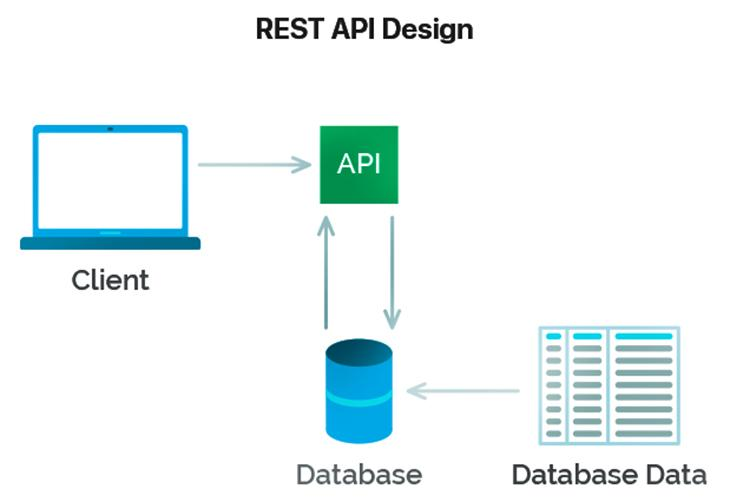
\includegraphics[width=0.75\textwidth]{Images/API.jpg}
    \vspace{1em}
    \caption{Mô hình kiến trúc Client-Server với REST API \cite{MicrosoftLearnClientServerImg}.}
    \label{fig:rest_api_architecture}
\end{figure}

\subsubsection{Frontend (Client)}
\label{subsubsec:frontend_component}
Frontend là lớp giao diện trực tiếp với người dùng, được xây dựng dưới dạng Single Page Application (SPA) để mang lại trải nghiệm mượt mà và nhanh chóng. Việc sử dụng React 18 kết hợp với các thư viện hiện đại như TanStack React Query cho quản lý state và Tailwind CSS cho styling giúp tăng tốc quá trình phát triển và đảm bảo chất lượng code.

Frontend được xây dựng bằng React 18 với các công nghệ chính:
\begin{itemize}
    \item \textbf{Core:} React 18, Vite (build tool), React Router Dom
    \item \textbf{API \& State:} Axios, TanStack React Query
    \item \textbf{Form:} React Hook Form, Yup validation
    \item \textbf{UI:} Tailwind CSS, DaisyUI
\end{itemize}
Cấu trúc thư mục: `pages`, `components`, `apis`, `contexts`, `hooks`, `utils`.

\subsubsection{Backend (Server)}
\label{subsubsec:backend_component}
Backend chịu trách nhiệm xử lý logic nghiệp vụ, quản lý dữ liệu và cung cấp API cho Frontend. Kiến trúc RESTful API module hóa giúp tách biệt rõ ràng các chức năng, dễ bảo trì và mở rộng. Việc sử dụng Node.js với Express.js không chỉ đảm bảo hiệu năng cao mà còn tạo sự đồng nhất ngôn ngữ JavaScript giữa Frontend và Backend, giúp đội ngũ phát triển làm việc hiệu quả hơn.

Backend xây dựng bằng Node.js và Express.js, cung cấp RESTful API module hóa:
\begin{itemize}
    \item \textbf{Nền tảng:} Node.js, Express.js, TypeScript
    \item \textbf{CSDL:} MongoDB (Mongoose ODM)
    \item \textbf{Xác thực:} JWT (JSON Web Tokens)
\end{itemize}

\textbf{Cấu trúc API Backend:} Các API được tổ chức theo tài nguyên:
\begin{itemize}
    \item `/api/auth`: Đăng ký, đăng nhập, bảo mật JWT
    \item `/api/users`: Quản lý hồ sơ, định danh tài khoản
    \item `/api/posts`, `/api/comments`: Quản lý bài đăng, phản hồi và mạng xã hội
    \item `/api/sport-events`: Quản lý sự kiện thể thao (tạo, chia sẻ, lưu tiến độ)
    \item `/api/challenges`: Quản trị chiến dịch thử thách cộng đồng
    \item `/api/workouts`, `/api/exercises`: Điều hướng bài tập và giáo án riêng
    \item `/api/ai`: Điều phối sinh thực thể từ Prompt, đo lường video camera
    \item `/api/calculator`: Tính toán sinh lý học (BMI, TDEE, BMR)
    \item `/api/calendar`: Đồng bộ trung tâm thời gian thực các sự kiện thể thao
    \item `/api/search`: Tìm kiếm truy vấn tổng hợp
    \item `/api/notifications`: Khởi tạo và phát luồng cảnh báo
\end{itemize}

\subsubsection{Cơ sở dữ liệu và Dịch vụ bổ trợ}
\label{subsubsec:database_support_services}
Lớp dữ liệu đóng vai trò quan trọng trong việc lưu trữ và quản lý thông tin. MongoDB được lựa chọn nhờ tính linh hoạt của schema, phù hợp với cấu trúc dữ liệu đa dạng của hệ thống mạng xã hội. Cloudinary cung cấp giải pháp lưu trữ ánh và video chuyên nghiệp, tự động tối ưu hóa và phân phối qua CDN toàn cầu, giúp giảm tải cho server chính và tăng tốc độ tải trang.

\begin{itemize}
    \item \textbf{MongoDB:} Lưu trữ chính cho toàn bộ hệ sinh thái dữ liệu (người dùng, bài đăng, sự kiện, thử thách, bài tập, tiến trình đồng bộ).
    \item \textbf{Cloudinary:} Dịch vụ lưu trữ đám mây cho hình ảnh, video.
\end{itemize}

% \subsection{Sơ đồ kiến trúc tổng quan hiện tại}
% \label{subsec:current_architecture_diagram}

% Sơ đồ dưới đây minh họa mối quan hệ giữa các thành phần chính trong kiến trúc hiện tại của hệ thống:

% \begin{figure}[H]
%     \centering
%     \includegraphics[width=0.9\textwidth]{Images/overall_architecture.png} % Thay bằng đường dẫn ảnh của bạn
%     \caption{Kiến trúc tổng thể hệ thống Nutrition Community Network (Nguồn: AWS Whitepapers - Minh họa)}
%     \label{fig:overall_architecture}
% \end{figure}
% *(Sơ đồ này cần thể hiện rõ: Client (React App) -> Giao tiếp qua REST API -> Backend (Node.js/Express - Module hóa) -> Tương tác với MongoDB, Redis, Cloudinary, và Socket.IO Server)*

% % \subsection{Luồng tương tác ví dụ: Tạo công thức nấu ăn}
% % \label{subsec:interaction_flow_recipe}

% % Luồng tương tác chi tiết khi người dùng tạo một công thức nấu ăn mới:

% % \begin{figure}[H]
% %     \centering
% %     \includegraphics[width=0.9\textwidth]{Images/interaction_flow.png} % Thay bằng đường dẫn ảnh của bạn
% %     \caption{Luồng tương tác giữa các thành phần khi tạo công thức (Minh họa)}
% %     \label{fig:interaction_flow}
% % \end{figure}

% % \begin{enumerate}
% %     \item \textbf{Người dùng (React App)} điền thông tin công thức (tên, nguyên liệu, hướng dẫn...) và chọn hình ảnh vào form.
% %     \item \textbf{React App (Client-side Validation)} sử dụng React Hook Form và Yup để kiểm tra tính hợp lệ của dữ liệu nhập.
% %     \item \textbf{React App (Image Upload)} gửi yêu cầu tải hình ảnh lên Cloudinary/Firebase Storage API.
% %     \item \textbf{Cloudinary/Firebase} xử lý, lưu trữ ảnh và trả về URL của ảnh đã lưu.
% %     \item \textbf{React App (API Request)} nhận URL ảnh, đóng gói dữ liệu công thức cùng URL ảnh và gửi yêu cầu POST đến `/api/recipes` trên \textbf{Backend Server}, kèm theo JWT token trong header Authorization.
% %     \item \textbf{Backend Server (Middleware)} xác thực JWT token.
% %     \item \textbf{Backend Server (Controller/Service)} nhận dữ liệu, thực hiện validation phía server.
% %     \item \textbf{Backend Server (Database Interaction)} lưu thông tin công thức mới vào collection `recipes` trong \textbf{MongoDB}.
% %     \item \textbf{Backend Server (Notification Logic - Async)} (Có thể) tạo bản ghi thông báo trong collection `notifications` và đẩy sự kiện "new_recipe" đến \textbf{Socket.IO Server}.
% %     \item \textbf{Socket.IO Server} phát thông báo "new_recipe" đến các client đang kết nối (ví dụ: những người theo dõi người đăng).
% %     \item \textbf{Backend Server} trả về phản hồi thành công (HTTP 201 Created) cho \textbf{React App}, kèm theo dữ liệu công thức vừa tạo (hoặc chỉ ID).
% %     \item \textbf{React App} nhận phản hồi, hiển thị thông báo thành công và điều hướng người dùng đến trang chi tiết công thức mới.
% % \end{enumerate}

\section{Thiết kế cơ sở dữ liệu}
\label{sec:database_design}

Hệ thống sử dụng MongoDB - cơ sở dữ liệu NoSQL hướng tài liệu, phù hợp với cấu trúc đa hình thái và đặc thù biến thiên của mạng xã hội thể thao. Thiết kế CSDL được tổ chức theo mô hình module hóa, chia thành 9 nhóm chức năng chính: Cộng đồng, Sự kiện thể thao, Thử thách cộng đồng, Công cụ tính toán, Tập luyện, Bạn bè, Lịch cá nhân và thông báo, Quản lý người dùng, và Quản lý hệ thống Admin. Thiết kế này giúp đảm bảo tính độc lập, dễ dàng bảo trì và hỗ trợ linh hoạt quá trình phát triển tương lai.

\subsection{Mô hình ERD tổng quan hệ thống}
\label{subsec:overall_erd}

Sơ đồ ERD (Entity-Relationship Diagram) tổng quan hệ thống phản ánh toàn bộ cấu trúc dữ liệu cốt lõi của nền tảng FitConnect, bao gồm các thực thể chính và mối quan hệ giữa chúng tương ứng với 9 nhóm tính năng được triển khai. Mô hình được thiết kế theo hướng tài liệu (Document-oriented) phù hợp với MongoDB, lấy thực thể \textbf{User} làm trung tâm liên kết, từ đó kết nối các nhánh nghiệp vụ độc lập theo từng phân hệ chức năng.

\begin{figure}[H]
    \centering
    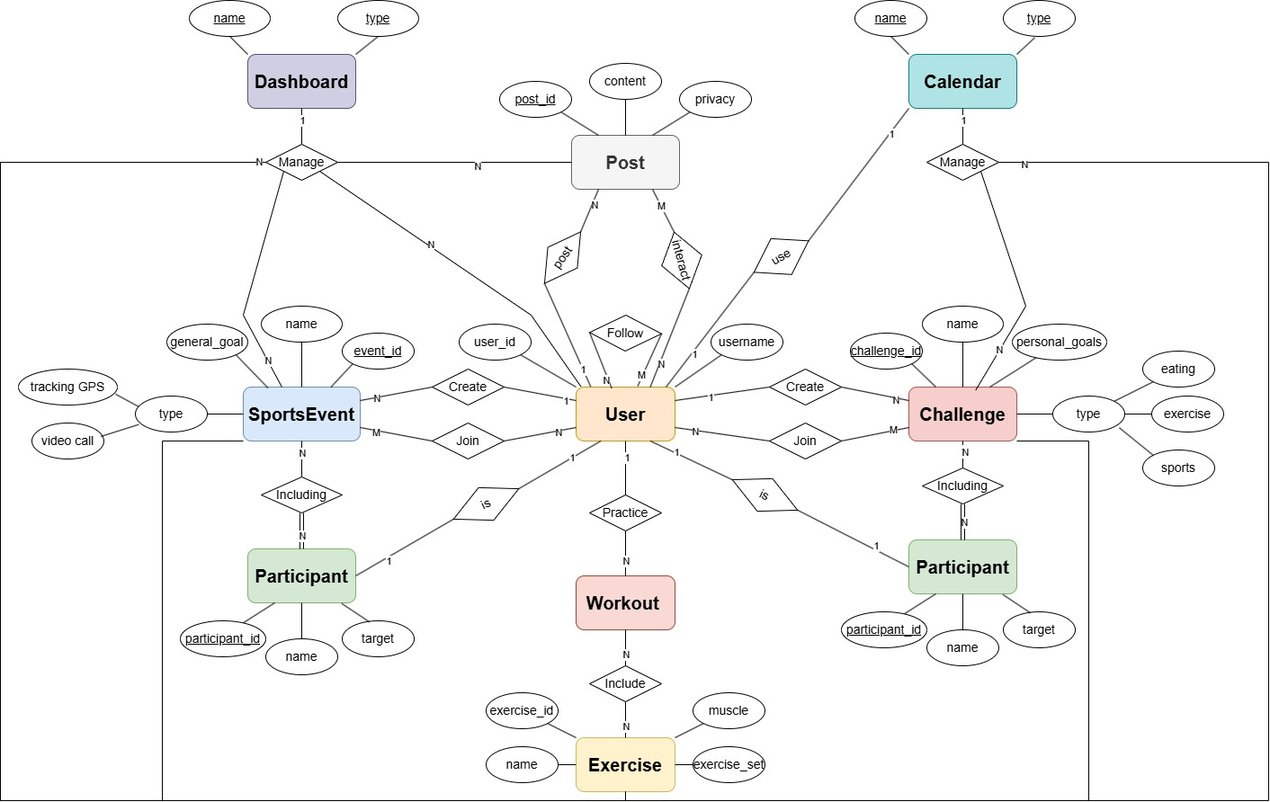
\includegraphics[width=1\textwidth]{Images/IMG/ERD/ERDTongquanhethong.jpg}
    \vspace{1em}
    \caption{Sơ đồ ERD tổng quan hệ thống: Thể hiện các thực thể chính, mối quan hệ và một số thuộc tính đại diện}
    \label{fig:erd_tongquan}
\end{figure}

\subsubsection{Các thực thể và vai trò của chúng trong hệ thống}
\label{subsubsec:erd_entities_roles}

Sơ đồ ERD tổng quan hệ thống gồm \textbf{10 thực thể chính}, lấy \textbf{User} làm trung tâm liên kết. Dưới đây là mô tả vai trò của từng thực thể trong hệ thống.

\begin{itemize}
    \item \textbf{User}: Thực thể trung tâm đại diện cho tài khoản người dùng trên nền tảng:
    \begin{itemize}
        \item Đăng bài chia sẻ hoạt động lên bảng tin cộng đồng (Community Feed).
        \item Bày tỏ cảm xúc (like) và bình luận vào bài viết của người khác.
        \item Theo dõi (Follow) các thành viên khác để xây dựng mạng lưới xã hội.
        \item Tạo hoặc tham gia các sự kiện thể thao và thử thách cộng đồng.
        \item Lập giáo án tập luyện cá nhân và theo dõi lịch trình qua lịch cá nhân.
    \end{itemize}

    \item \textbf{Post}: Đại diện cho các bài đăng trên bảng tin cộng đồng:
    \begin{itemize}
        \item Thuộc về một người dùng duy nhất, có thể đính kèm hình ảnh hoặc video.
        \item Kiểm soát phạm vi hiển thị: công khai, chỉ bạn bè hoặc riêng tư.
        \item Nhận tương tác từ người dùng khác qua cảm xúc (like) và bình luận (comment).
    \end{itemize}

    \item \textbf{SportsEvent}: Lưu trữ thông tin các sự kiện thể thao tập thể:
    \begin{itemize}
        \item Được tạo bởi một người dùng và cho phép nhiều người dùng khác đăng ký tham gia.
        \item Hỗ trợ hai hình thức: \textit{Ngoài trời} (ghi nhận lộ trình GPS thời gian thực) và \textit{Trong nhà} (Video Call nhóm tích hợp nhận diện khuôn mặt AI).
        \item Quản lý danh sách người tham gia thông qua thực thể \textbf{Participant (SportsEvent)}.
    \end{itemize}

    \item \textbf{Participant (SportsEvent)}: Thực thể trung gian ghi nhận thông tin tham dự sự kiện:
    \begin{itemize}
        \item Được tạo ra khi một người dùng tham gia một sự kiện thể thao.
        \item Lưu trữ mục tiêu cá nhân và tiến độ thi đua của từng thành viên.
        \item Phục vụ xây dựng bảng xếp hạng nội bộ sự kiện.
    \end{itemize}

    \item \textbf{Challenge}: Quản lý các thử thách rèn luyện kỷ luật ngắn hạn trong cộng đồng:
    \begin{itemize}
        \item Được tạo thủ công bởi người dùng hoặc do AI tự động đề xuất nội dung.
        \item Phân thành ba loại: dinh dưỡng (eating), bài tập (exercise) và thể thao ngoài trời (sports).
        \item Cho phép nhiều người dùng cùng tham gia và check-in tiến độ hằng ngày.
    \end{itemize}

    \item \textbf{Participant (Challenge)}: Thực thể trung gian ghi nhận check-in thử thách hằng ngày:
    \begin{itemize}
        \item Lưu lại mục tiêu cá nhân và kết quả hoàn thành từng ngày.
        \item Phục vụ tính toán bảng xếp hạng nội bộ thử thách.
    \end{itemize}

    \item \textbf{Workout}: Đại diện cho một giáo án tập luyện cá nhân:
    \begin{itemize}
        \item Được người dùng tự tạo hoặc do AI đề xuất dựa trên chỉ số sức khỏe.
        \item Bao gồm danh sách các bài tập cụ thể liên kết qua thực thể \textbf{Exercise}.
        \item Có thể lưu vào lịch tập luyện và theo dõi lịch sử hoạt động.
    \end{itemize}

    \item \textbf{Exercise}: Kho dữ liệu kỹ thuật của tất cả bài tập đơn lẻ trong hệ thống:
    \begin{itemize}
        \item Chỉ định nhóm cơ mục tiêu và mô tả kỹ thuật thực hành.
        \item Lưu cấu hình hiệp/lần/thời gian cho từng bài tập.
        \item Được các giáo án \textbf{Workout} tham chiếu để xây dựng lộ trình cá nhân hóa.
    \end{itemize}

    \item \textbf{Dashboard}: Phân hệ quản trị dành riêng cho Admin:
    \begin{itemize}
        \item Theo dõi các chỉ số tăng trưởng nền tảng qua biểu đồ trực quan.
        \item Quản lý toàn bộ người dùng và sự kiện thể thao trên hệ thống.
        \item Xem xét và xử lý báo cáo vi phạm nội dung từ cộng đồng.
        \item Cấu hình danh mục thể thao làm tiêu chuẩn phân loại toàn hệ thống.
    \end{itemize}

    \item \textbf{Calendar}: Lịch cá nhân tổng hợp của người dùng:
    \begin{itemize}
        \item Tự động tổng hợp các mốc thời gian từ sự kiện thể thao, thử thách và lịch tập luyện.
        \item Hiển thị toàn bộ lịch trình trong một giao diện thống nhất.
        \item Gửi thông báo nhắc nhở đúng thời điểm khi đến hạn thực hiện mục tiêu.
    \end{itemize}
\end{itemize}


\subsubsection{Tổng kết mối quan hệ giữa các thực thể}
\label{subsubsec:erd_relationships_summary}
Bảng dưới đây tóm tắt các mối quan hệ chính trong sơ đồ ERD tổng quan:

\begin{table}[H]
\centering
\caption{Tổng kết quan hệ trong sơ đồ ERD tổng quan hệ thống}
\label{tab:erd_relationships}
\begin{tabular}{|l|l|c|l|}
\hline
\textbf{Thực thể A} & \textbf{Thực thể B} & \textbf{Lực lượng} & \textbf{Tên quan hệ} \\
\hline
User & Post & 1 -- N & post (đăng bài) \\
User & Post & M -- M & interact (tương tác) \\
User & User & M -- M & Follow (theo dõi) \\
User & SportsEvent & 1 -- N & Create (tạo sự kiện) \\
User & SportsEvent & M -- N & Join (tham gia sự kiện) \\
SportsEvent & Participant (Event) & 1 -- N & Including \\
User & Participant (Event) & 1 -- 1 & is \\
User & Challenge & 1 -- N & Create (tạo thử thách) \\
User & Challenge & 1 -- M & Join (tham gia thử thách) \\
Challenge & Participant (Chall.) & 1 -- N & Including \\
User & Participant (Chall.) & 1 -- 1 & is \\
User & Workout & 1 -- N & Practice (tập luyện) \\
Workout & Exercise & N -- N & Include \\
User & Calendar & 1 -- N & use (sử dụng lịch) \\
Dashboard & SportsEvent / User & 1 -- N & Manage (quản lý) \\
Calendar & User & 1 -- N & Manage (quản lý lịch) \\
\hline
\end{tabular}
\end{table}

\subsection{Phân tích 9 nhóm chức năng chính (Module)}
\label{subsec:main_modules_analysis}

Dựa trên sơ đồ ERD tổng quan và nguyên tắc thiết kế hướng tài liệu (Document-oriented) của MongoDB, cơ sở dữ liệu được tổ chức thành 9 nhóm tính năng chính. Mỗi nhóm sở hữu tập hợp các collection riêng biệt, đảm bảo tính độc lập trong truy vấn và khả năng mở rộng linh hoạt.

% ─── 1. QUẢN LÝ NGƯỜI DÙNG ──────────────────────────────────────────────────
\subsubsection{Nhóm tính năng Quản lý người dùng}
\label{subsubsec:module_nguoidung}

Nhóm này đóng vai trò nền tảng định danh của toàn hệ thống, quản lý vòng đời tài khoản từ đăng ký, xác thực đến lưu trữ hồ sơ sức khỏe cá nhân. Mọi collection nghiệp vụ khác trong hệ thống đều tham chiếu về user\_id của nhóm này như một khóa ngoại xuyên suốt.

\begin{figure}[H]
    \centering
    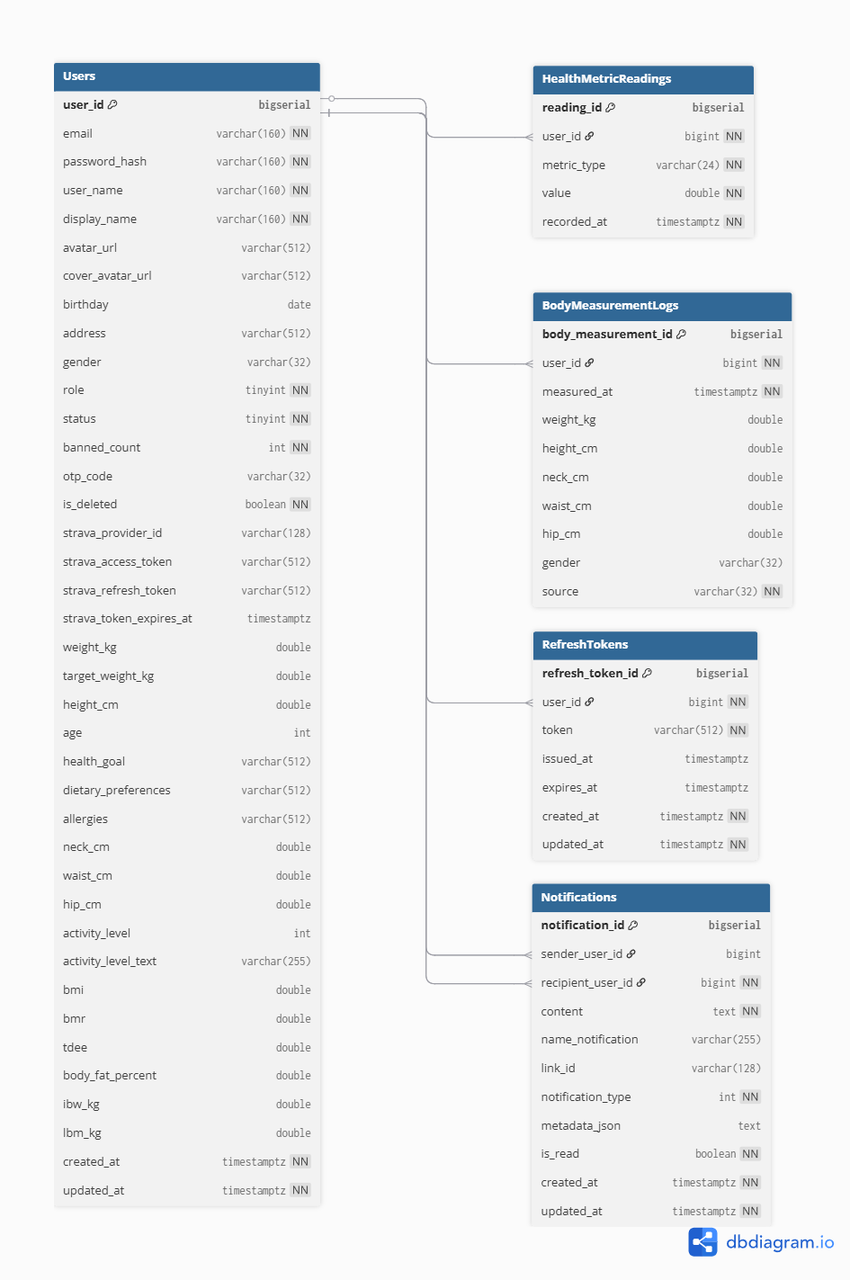
\includegraphics[width=0.85\textwidth]{Images/IMG/ERD/ERDQuanlynguoidung.png}
    \vspace{1em}
    \caption{ERD nhóm tính năng Quản lý người dùng}
    \label{fig:erd_nguoidung}
\end{figure}

\textbf{Các collection chính và chức năng:}
\begin{itemize}
    \item \textbf{users:} Lưu trữ toàn bộ thông tin tài khoản và hồ sơ cá nhân, bao gồm thông tin định danh (email, tên hiển thị, ảnh đại diện, ngày sinh, giới tính), phân quyền và trạng thái tài khoản. Ngoài ra còn lưu các chỉ số sức khỏe tích hợp như cân nặng, chiều cao, BMI, BMR, TDEE, tỷ lệ mỡ cơ thể và các tùy chọn cá nhân hóa.
    \item \textbf{health\_metric\_readings:} Ghi nhận chuỗi lịch sử các chỉ số sức khỏe theo thời gian (loại chỉ số, giá trị đo, thời điểm ghi nhận), phục vụ vẽ biểu đồ xu hướng thể trạng.
    \item \textbf{body\_measurement\_logs:} Lưu lịch sử đo lường cơ thể định kỳ (cân nặng, chiều cao, vòng cổ, vòng eo, vòng hông), hỗ trợ tính toán chỉ số mỡ cơ thể và theo dõi tiến độ giảm cân.
    \item \textbf{refresh\_tokens:} Quản lý phiên đăng nhập bảo mật theo cơ chế JWT Refresh Token, lưu thông tin token, thời điểm cấp phát và thời hạn hết hiệu lực, đảm bảo xác thực liên tục và an toàn.
    \item \textbf{notifications:} Lưu trữ và phân phối thông báo hệ thống tới người dùng, bao gồm loại thông báo, nội dung, liên kết điều hướng và trạng thái đã đọc, hỗ trợ thông báo thời gian thực.
\end{itemize}

% ─── 2. CỘNG ĐỒNG ─────────────────────────────────────────────────────────────
\subsubsection{Nhóm tính năng Cộng đồng}
\label{subsubsec:module_congdong}

Nhóm này kiến tạo không gian mạng xã hội tương tác mở, cho phép người dùng chia sẻ hoạt động, tương tác bài viết và xây dựng mạng lưới quan hệ. Đây là trung tâm nội dung sôi động nhất của nền tảng, tích hợp kiểm duyệt AI tự động để đảm bảo môi trường lành mạnh.

\begin{figure}[H]
    \centering
    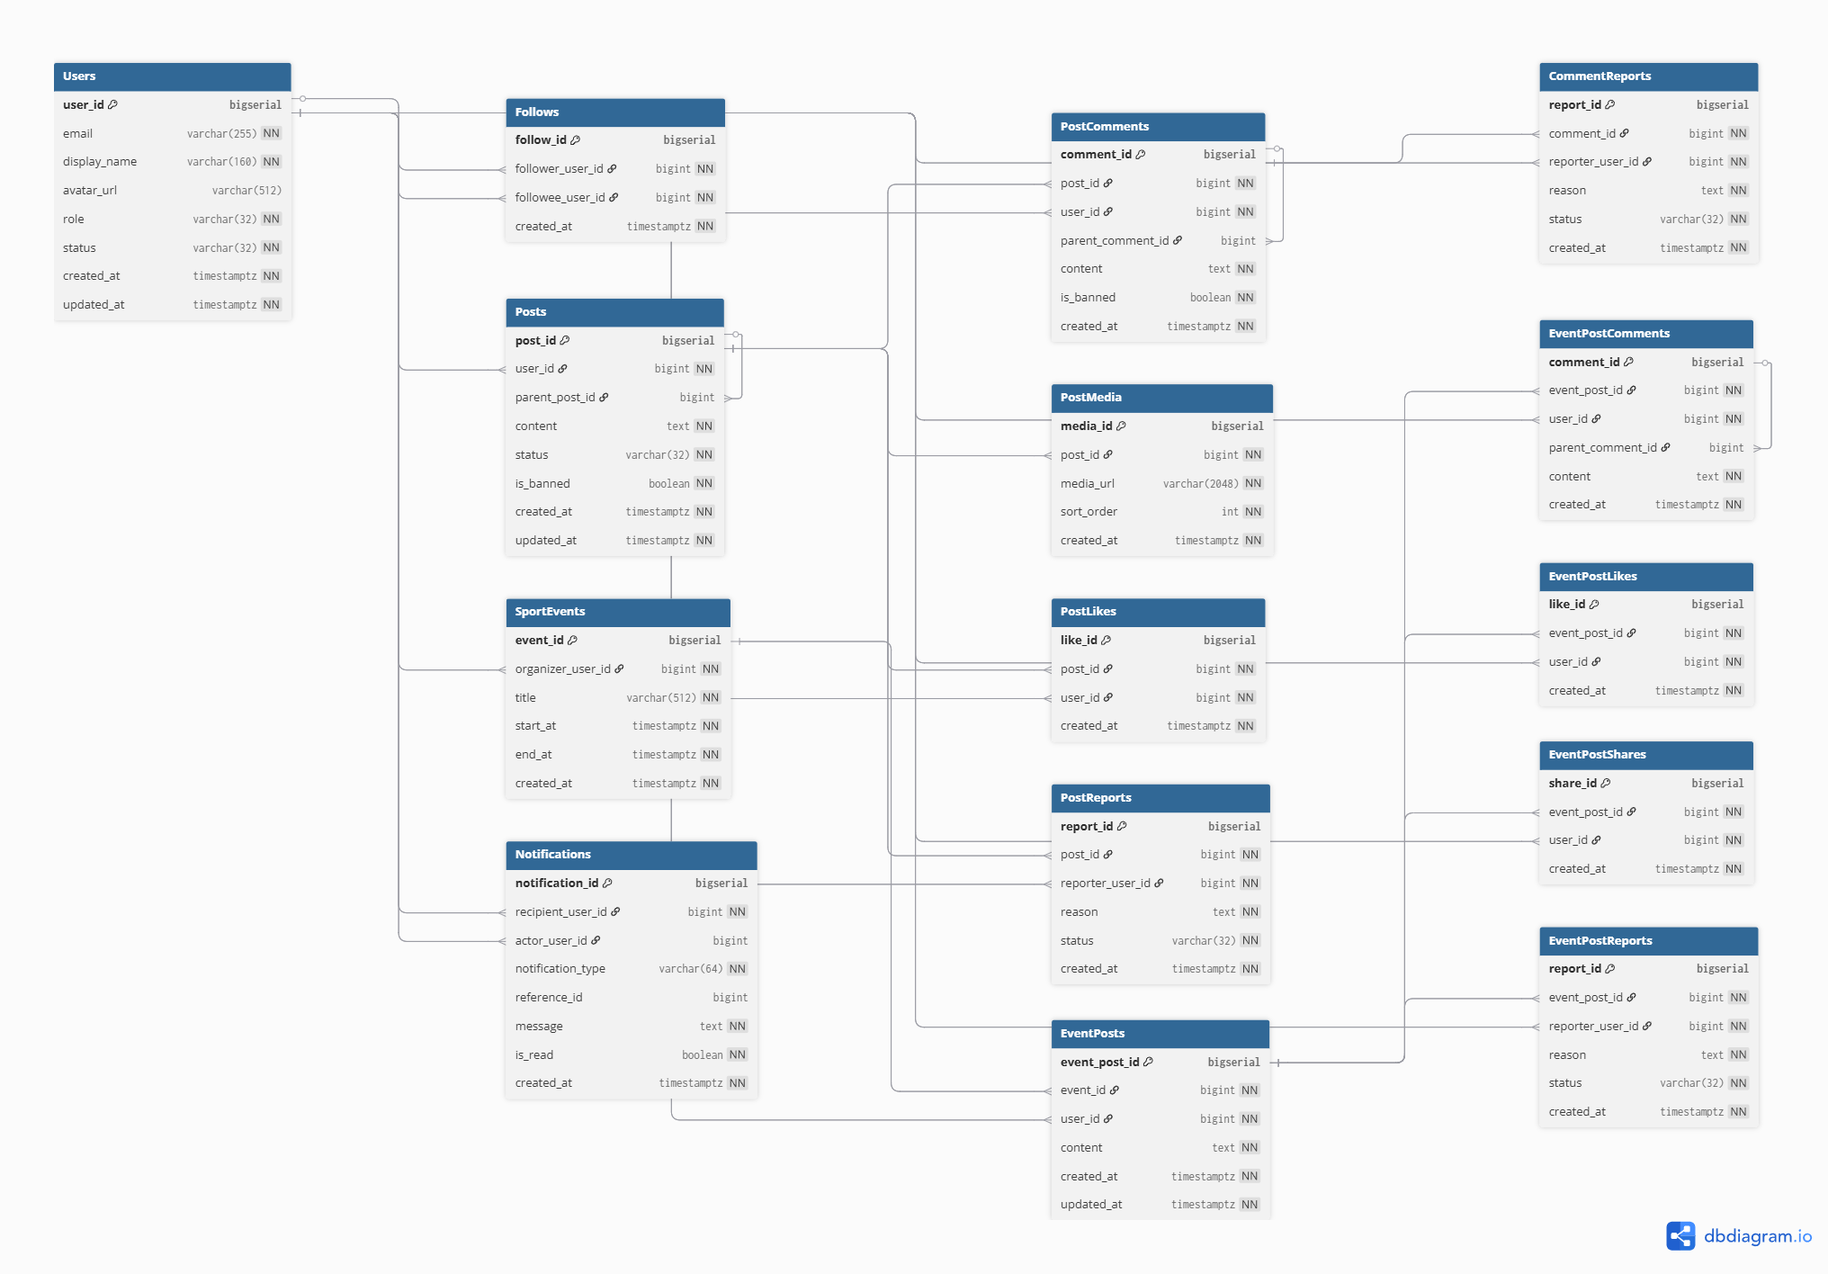
\includegraphics[width=1\textwidth]{Images/IMG/ERD/ERDCongDong.png}
    \vspace{1em}
    \caption{ERD nhóm tính năng Cộng đồng}
    \label{fig:erd_congdong}
\end{figure}

\textbf{Các collection chính và chức năng:}
\begin{itemize}
    \item \textbf{posts:} Lưu trữ bài viết của người dùng trên bảng tin cộng đồng, bao gồm nội dung văn bản, trạng thái kiểm duyệt và liên kết chia sẻ lại từ bài viết gốc. Hỗ trợ cấu trúc bài viết phân cấp (chia sẻ lại).
    \item \textbf{post\_media:} Quản lý tệp đính kèm đa phương tiện (hình ảnh, video) của từng bài viết, hỗ trợ sắp xếp thứ tự hiển thị nhiều ảnh trên một bài đăng.
    \item \textbf{post\_likes:} Ghi nhận lượt thích của từng người dùng với từng bài viết, đảm bảo tính duy nhất mỗi tương tác.
    \item \textbf{post\_comments:} Lưu trữ bình luận phân cấp, hỗ trợ trả lời lồng nhau và trạng thái kiểm duyệt từng bình luận.
    \item \textbf{post\_reports / comment\_reports:} Tiếp nhận báo cáo vi phạm bài viết và bình luận từ cộng đồng (lý do, trạng thái xử lý), cung cấp dữ liệu cho Admin kiểm duyệt.
    \item \textbf{follows:} Quản lý quan hệ theo dõi một chiều giữa người dùng (ai theo dõi ai), phục vụ lọc và phân phối bài viết ưu tiên từ mạng lưới bạn bè trên bảng tin.
    \item \textbf{event\_posts:} Tập hợp collection song song cho phép người tham gia sự kiện chia sẻ kết quả, cảm nghĩ lên bảng tin cộng đồng, tích hợp like, bình luận và báo cáo tương tự posts thông thường.
\end{itemize}

% ─── 3. SỰ KIỆN THỂ THAO ─────────────────────────────────────────────────────
\subsubsection{Nhóm tính năng Sự kiện thể thao}
\label{subsubsec:module_sukien}

Nhóm này điều phối toàn bộ vòng đời của các sự kiện thể thao tập thể: từ khi tổ chức viên tạo sự kiện, người dùng tham gia, ghi nhận tiến độ theo thời gian thực (GPS hoặc Video Call), cho đến khi chia sẻ kết quả lên cộng đồng.

\begin{figure}[H]
    \centering
    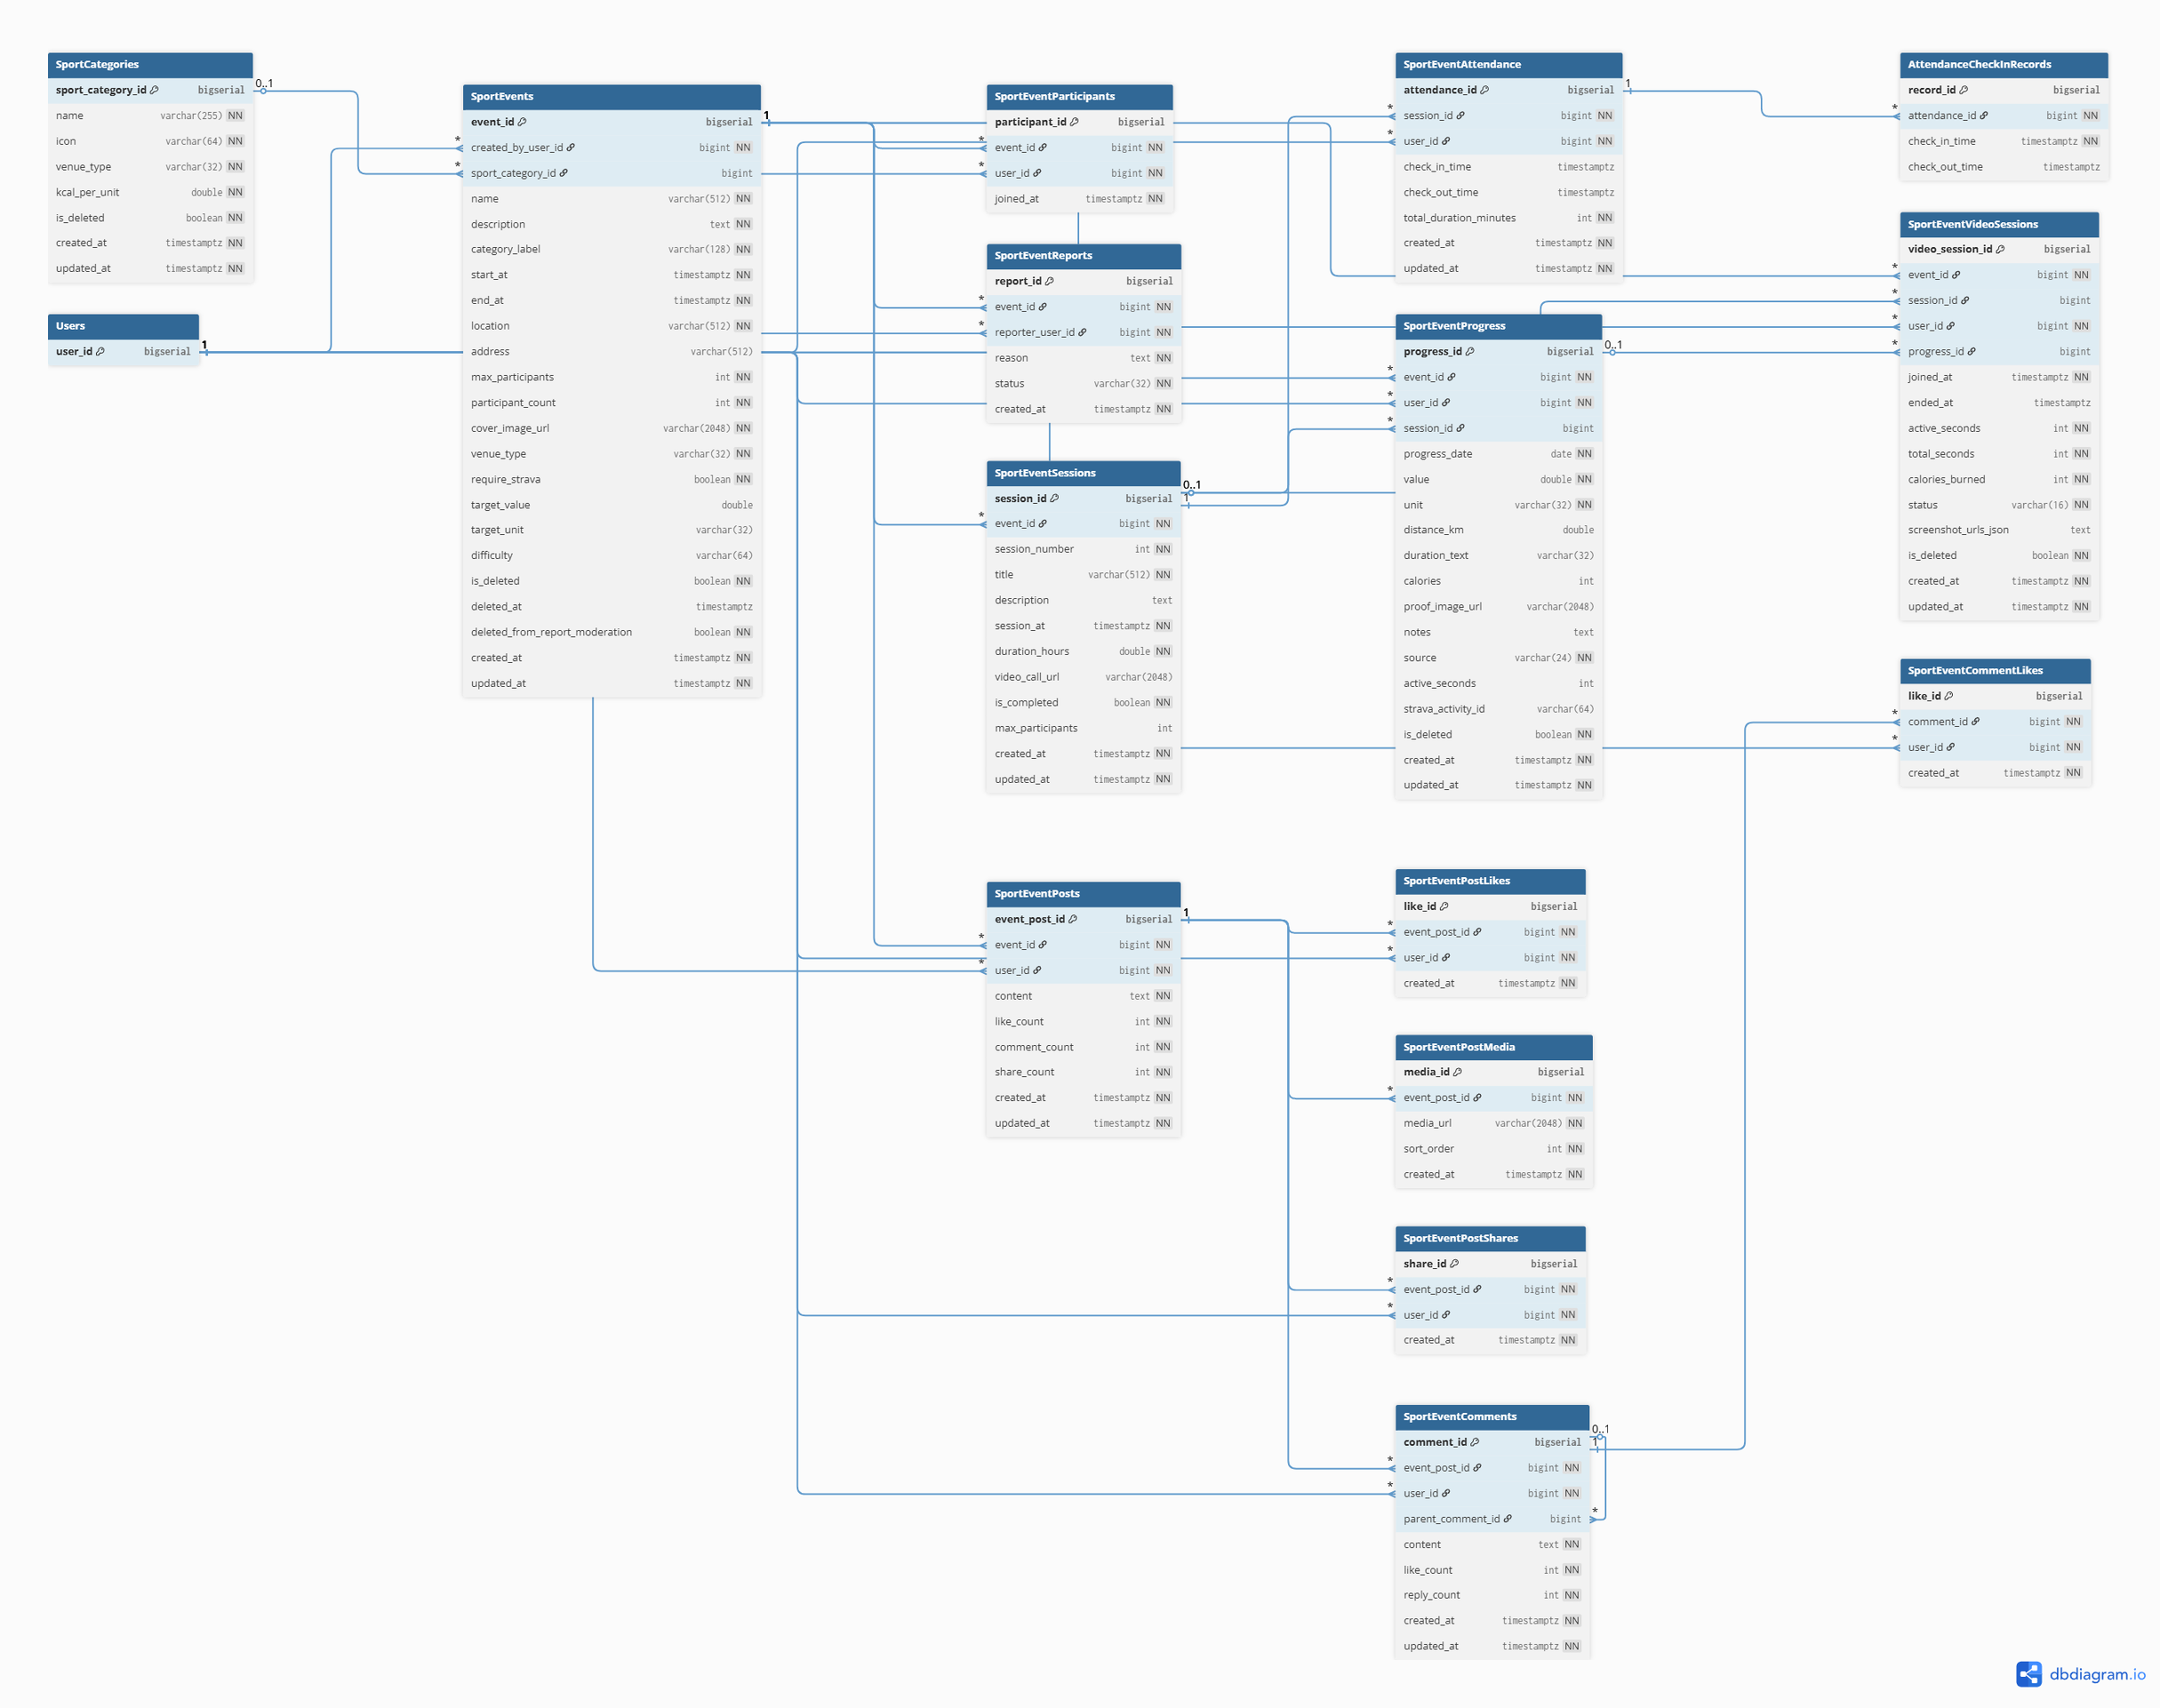
\includegraphics[width=1\textwidth]{Images/IMG/ERD/ERDSukienthethao.png}
    \vspace{1em}
    \caption{ERD nhóm tính năng Sự kiện thể thao}
    \label{fig:erd_sukien}
\end{figure}

\textbf{Các collection chính và chức năng:}
\begin{itemize}
    \item \textbf{sport\_categories:} Danh mục phân loại thể thao do Admin cấu hình, lưu tên môn, kiểu địa điểm (trong nhà/ngoài trời) và lượng calo tiêu hao chuẩn, làm tiêu chuẩn phân loại chung toàn hệ thống.
    \item \textbf{sport\_events:} Định nghĩa đầy đủ thông tin sự kiện: tên, mô tả, thời gian bắt đầu/kết thúc, địa điểm, giới hạn người tham gia, hình thức (trong nhà/ngoài trời), mục tiêu và độ khó.
    \item \textbf{sport\_event\_participants:} Lưu thông tin đăng ký tham gia của từng người dùng vào sự kiện, bao gồm thời điểm đăng ký.
    \item \textbf{sport\_event\_sessions:} Đại diện cho từng buổi thi đấu trong sự kiện, lưu số thứ tự buổi, thời gian, thời lượng, đường dẫn phòng Video Call và trạng thái hoàn thành.
    \item \textbf{sport\_event\_progress:} Ghi nhận kết quả thi đua của từng người dùng trong từng buổi (giá trị đạt được, quãng đường, lượng calo, ảnh bằng chứng).
    \item \textbf{sport\_event\_attendance / attendance\_check\_in\_records:} Theo dõi và lưu chi tiết điểm danh từng phiên theo thời gian vào/ra, phục vụ tính tổng thời lượng tham gia thực tế.
    \item \textbf{sport\_event\_video\_sessions:} Quản lý thông tin phòng Video Call nhóm, ghi nhận thời gian người dùng tham gia qua camera và tổng thời gian hoạt động.
    \item \textbf{sport\_event\_posts / sport\_event\_comments:} Cho phép người tham gia chia sẻ cảm nghĩ và tương tác trong không gian riêng của từng sự kiện.
\end{itemize}

% ─── 4. THỬ THÁCH CỘNG ĐỒNG ──────────────────────────────────────────────────
\subsubsection{Nhóm tính năng Thử thách cộng đồng}
\label{subsubsec:module_thuthach}

Nhóm này quản lý các chiến dịch rèn luyện kỷ luật theo ngày trong cộng đồng. Người dùng check-in tiến độ hằng ngày theo phương thức đặc thù của từng loại thử thách; AI tự động xác thực dữ liệu đầu vào và cập nhật bảng xếp hạng theo thời gian thực.

\begin{figure}[H]
    \centering
    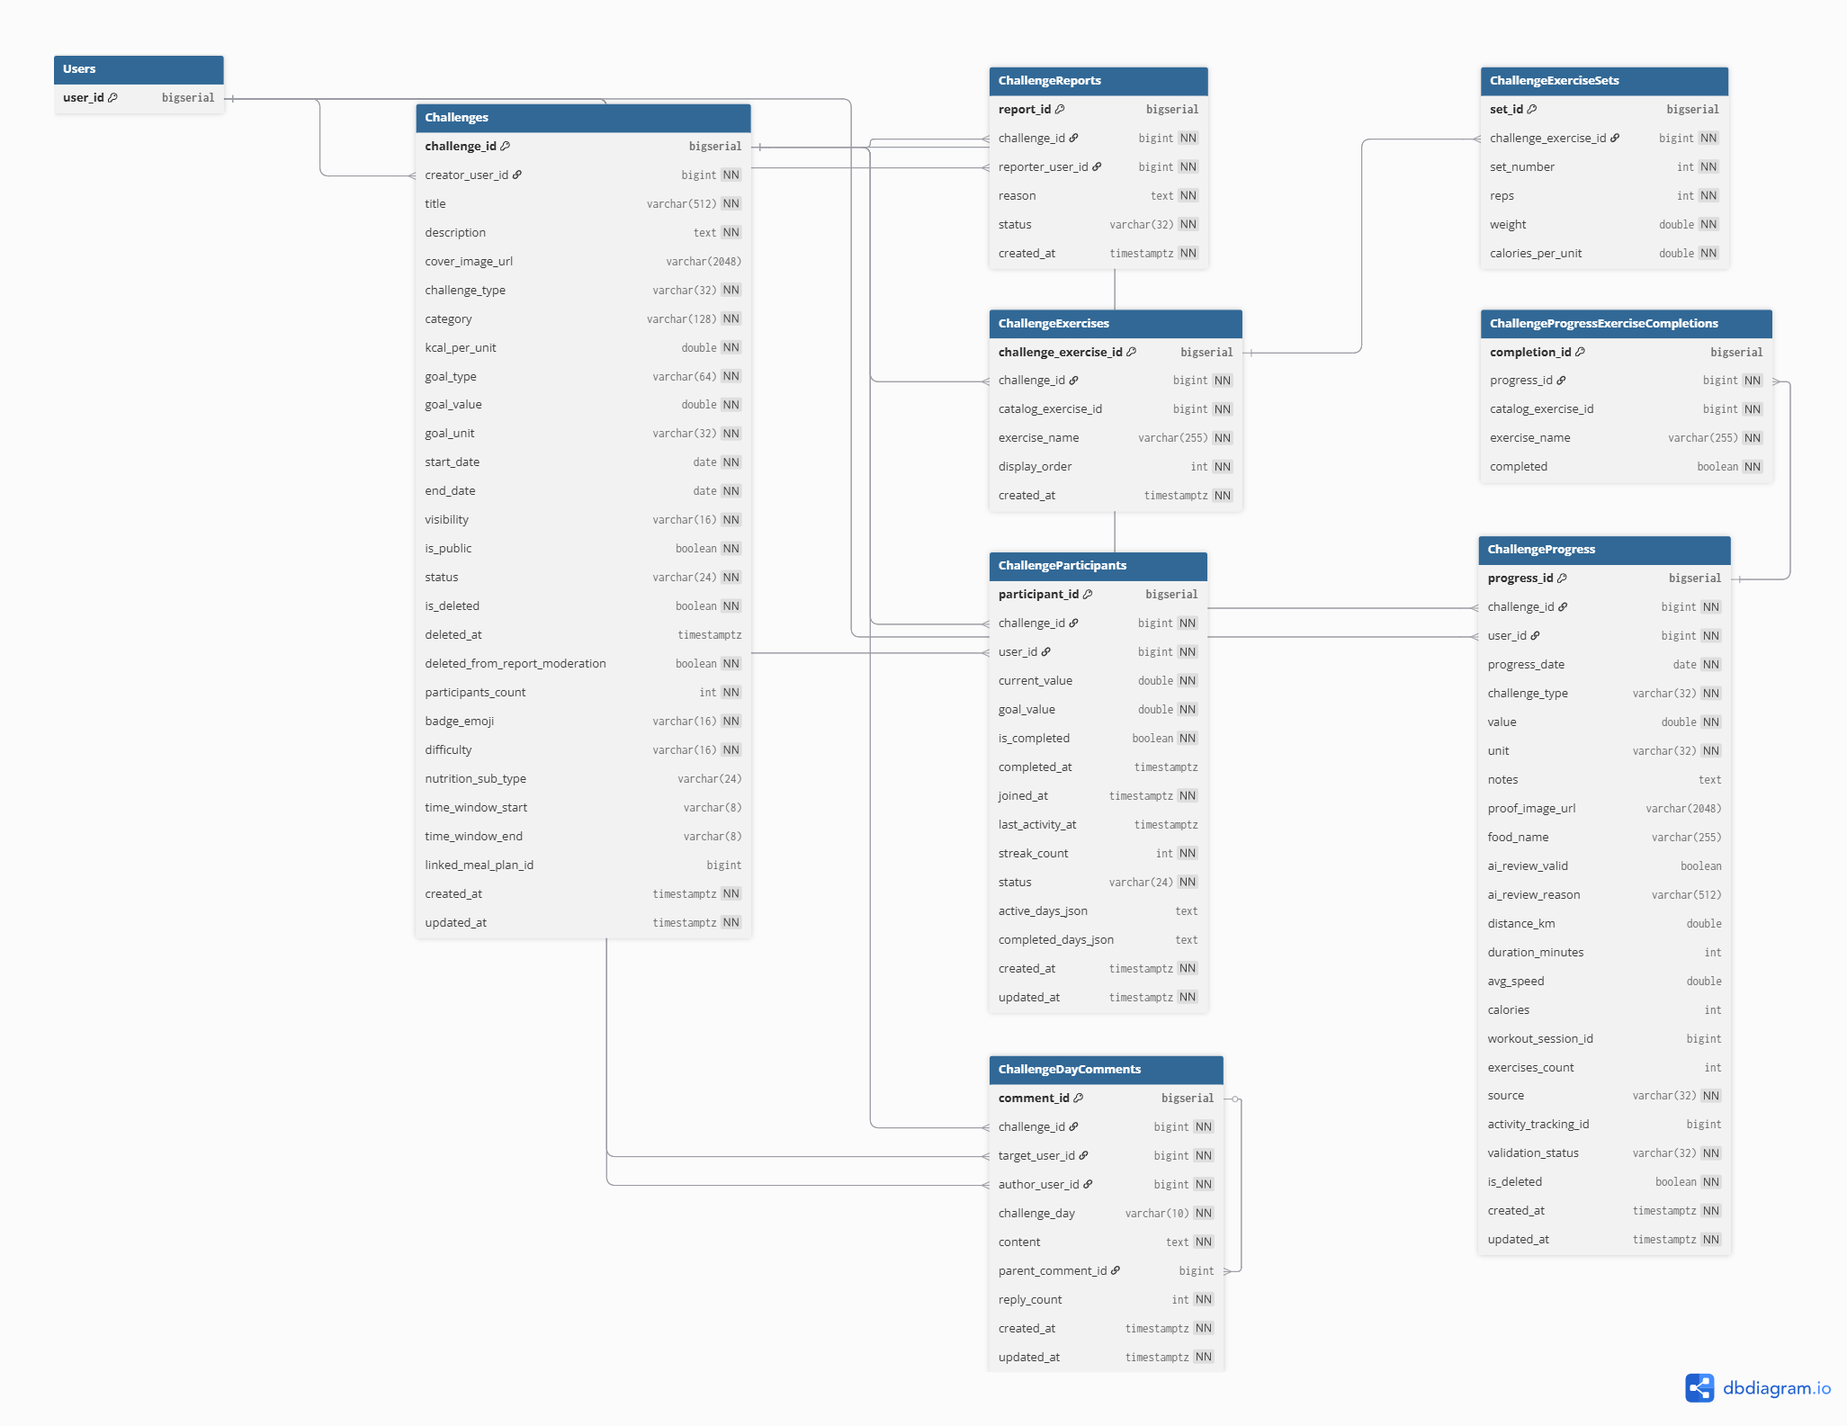
\includegraphics[width=1\textwidth]{Images/IMG/ERD/ERDThuthachcongdong.png}
    \vspace{1em}
    \caption{ERD nhóm tính năng Thử thách cộng đồng}
    \label{fig:erd_thuthach}
\end{figure}

\textbf{Các collection chính và chức năng:}
\begin{itemize}
    \item \textbf{challenges:} Định nghĩa thử thách với đầy đủ thông tin: tên, mô tả, loại thử thách (dinh dưỡng, bài tập, thể thao), mục tiêu cần đạt, ngày bắt đầu/kết thúc, phạm vi hiển thị và khung giờ thực hiện trong ngày.
    \item \textbf{challenge\_participants:} Ghi nhận trạng thái tham gia của từng người dùng, theo dõi giá trị hiện tại so với mục tiêu, số ngày streak liên tiếp, ngày hoạt động và trạng thái hoàn thành tổng thể.
    \item \textbf{challenge\_progress:} Lưu chi tiết mỗi lần check-in hằng ngày: ngày thực hiện, giá trị đạt được, ghi chú, ảnh bằng chứng, kết quả xác thực của AI, thông tin vận động (quãng đường, thời gian, lượng calo) và tên thực phẩm nếu là thử thách dinh dưỡng.
    \item \textbf{challenge\_exercises / challenge\_exercise\_sets:} Liệt kê danh sách bài tập yêu cầu và cấu hình hiệp/lần/cân nặng cho từng bài tập trong thử thách dạng vận động.
    \item \textbf{challenge\_day\_comments:} Cho phép người tham gia bình luận, động viên nhau gắn với ngày check-in cụ thể, hỗ trợ trả lời lồng nhau.
    \item \textbf{challenge\_reports:} Tiếp nhận báo cáo vi phạm thử thách từ cộng đồng để Admin xem xét.
\end{itemize}

% ─── 5. TẬP LUYỆN ─────────────────────────────────────────────────────────────
\subsubsection{Nhóm tính năng Tập luyện}
\label{subsubsec:module_tapluyen}

Nhóm này phục vụ nhu cầu tập luyện cá nhân độc lập, cung cấp kho bài tập phong phú, công cụ lập giáo án (thủ công hoặc AI đề xuất), ghi nhận buổi tập thực tế và theo dõi lịch sử hoạt động theo thời gian.

\begin{figure}[H]
    \centering
    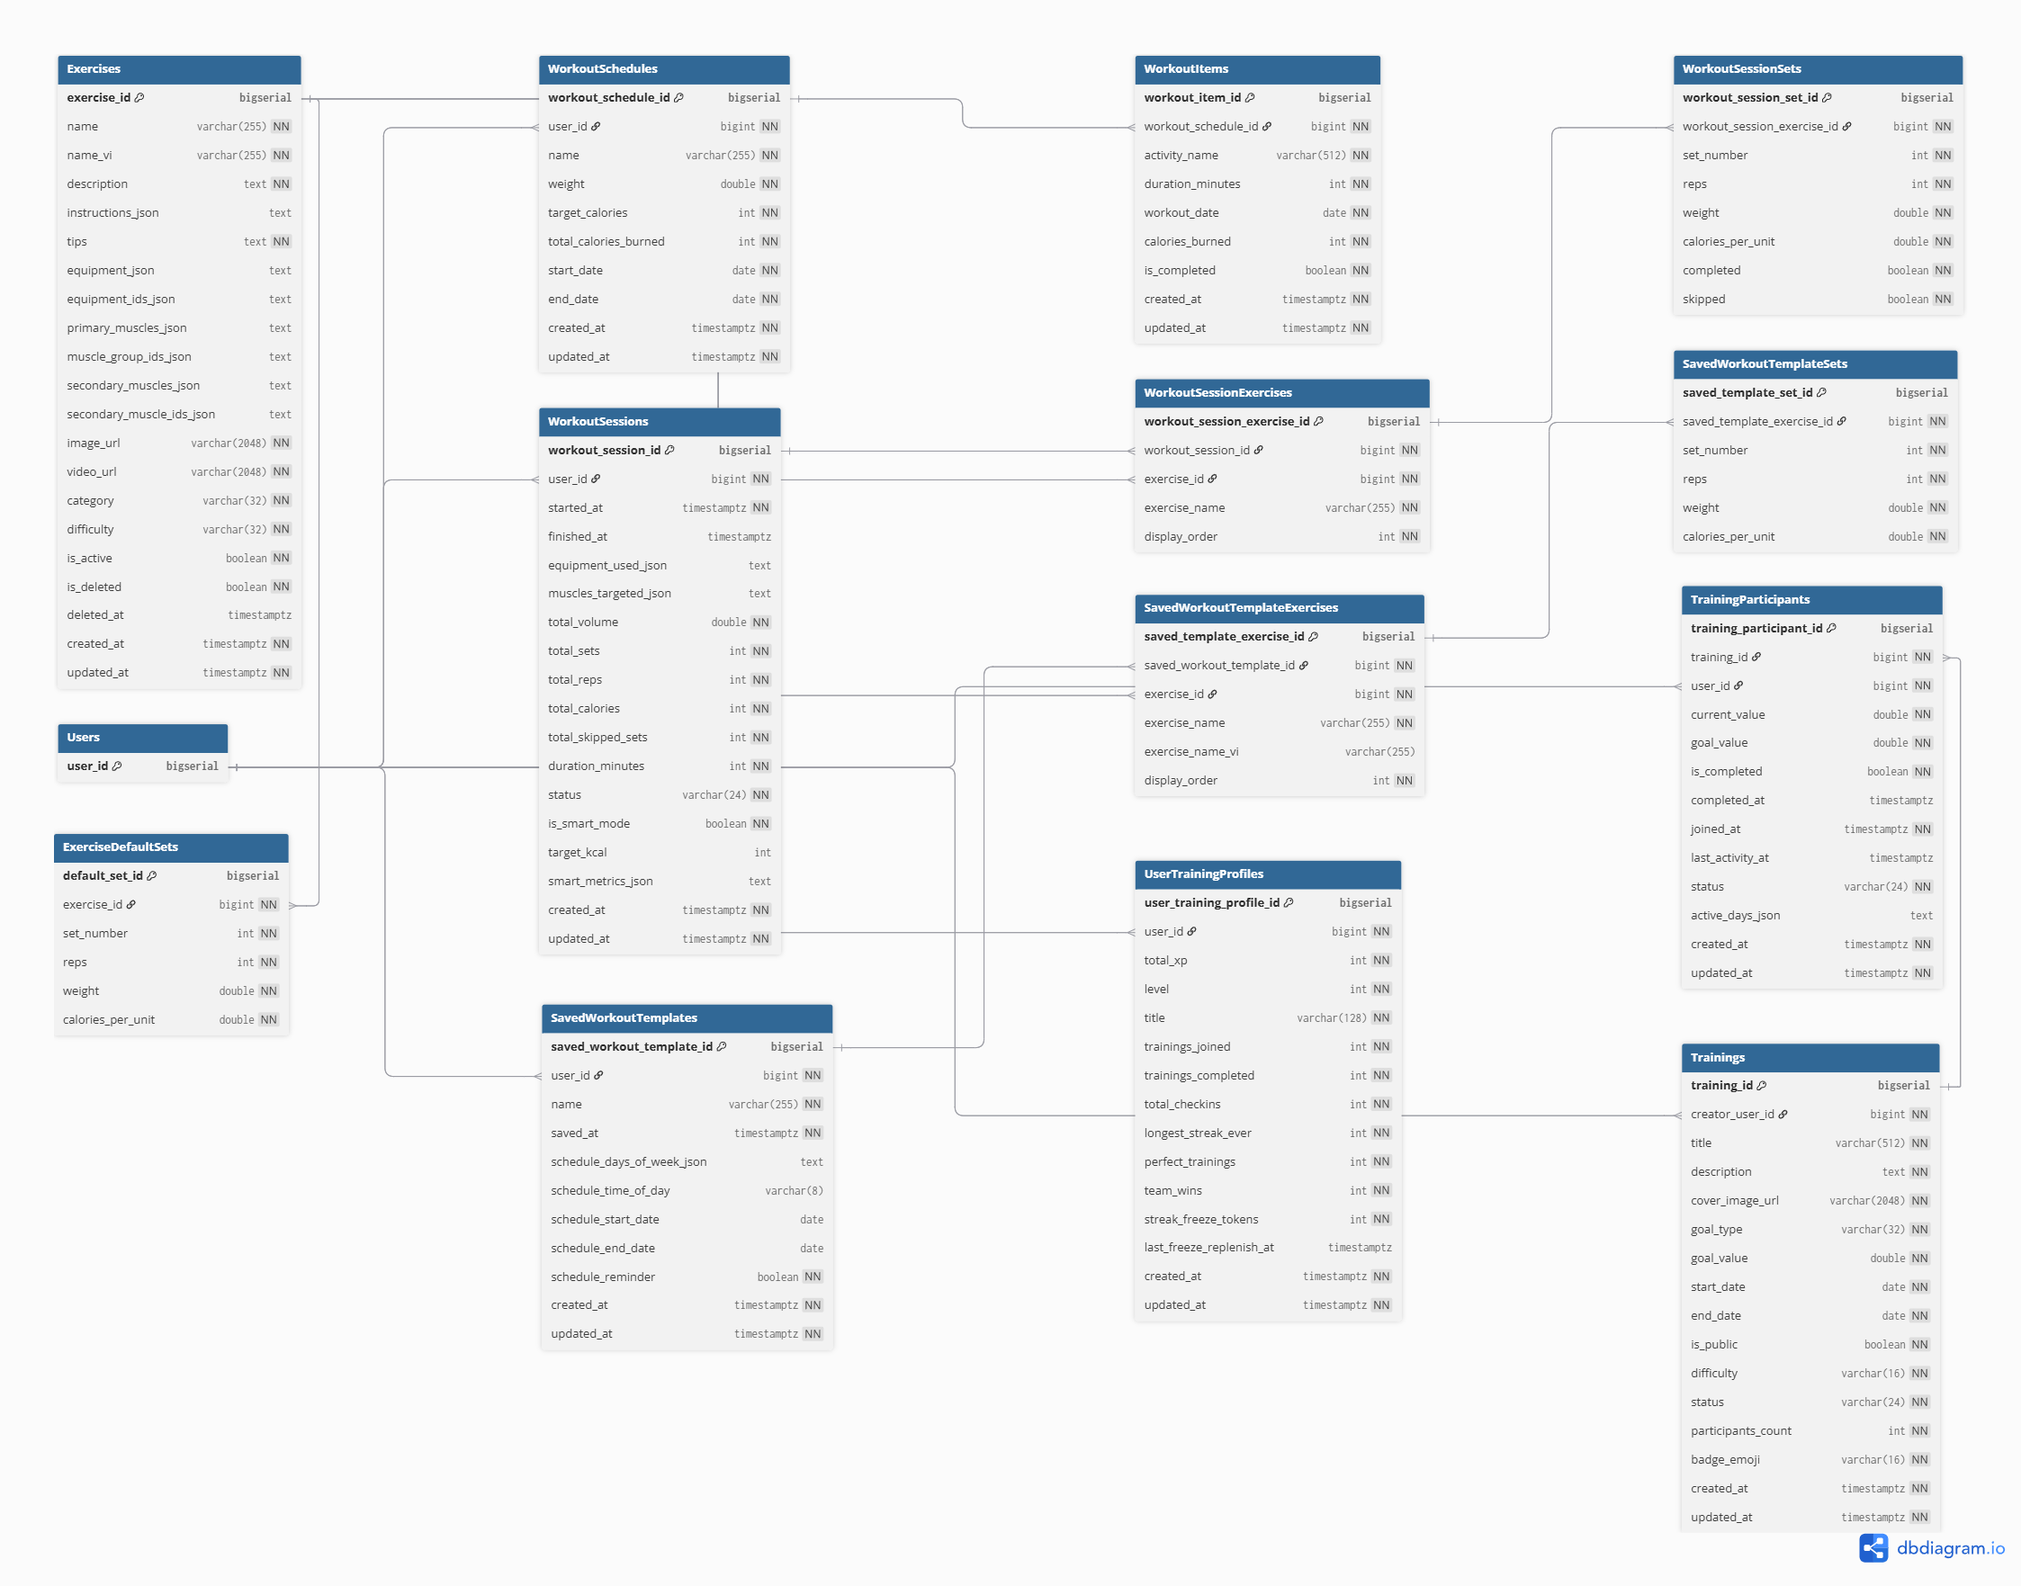
\includegraphics[width=1\textwidth]{Images/IMG/ERD/ERDTapluyen.png}
    \vspace{1em}
    \caption{ERD nhóm tính năng Tập luyện}
    \label{fig:erd_tapluyen}
\end{figure}

\textbf{Các collection chính và chức năng:}
\begin{itemize}
    \item \textbf{exercises:} Kho bài tập hệ thống với đầy đủ thông tin kỹ thuật: tên bài tập, mô tả, hướng dẫn thực hiện từng bước, mẹo, danh sách thiết bị, nhóm cơ chính/phụ được tác động, hình ảnh minh họa, video hướng dẫn, phân loại và mức độ khó.
    \item \textbf{workout\_sessions:} Ghi nhận buổi tập thực tế của người dùng, lưu thời gian bắt đầu/kết thúc, tổng khối lượng, số hiệp, số lần, lượng calo tiêu hao, thời lượng tập và chế độ thông minh (AI-guided).
    \item \textbf{workout\_session\_exercises / workout\_session\_sets:} Liệt kê chi tiết các bài tập và từng hiệp thực tế trong buổi tập (số hiệp, số lần, cân nặng, trạng thái hoàn thành hoặc bỏ qua).
    \item \textbf{workout\_schedules / workout\_items:} Quản lý giáo án tập luyện được lên kế hoạch theo tuần/tháng và danh sách các hoạt động tập luyện theo ngày cụ thể trong lịch.
    \item \textbf{saved\_workout\_templates:} Giáo án mẫu đã lưu để tái sử dụng, hỗ trợ lặp lại theo ngày trong tuần, khung giờ tập và tùy chọn nhắc nhở tự động.
    \item \textbf{user\_training\_profiles:} Hồ sơ tập luyện gamification của người dùng, theo dõi điểm kinh nghiệm (XP), cấp độ, danh hiệu, số buổi tập đã tham gia/hoàn thành và streak dài nhất.
    \item \textbf{trainings / training\_participants:} Hỗ trợ hình thức tập luyện theo nhóm với cơ chế tham gia và theo dõi tiến độ tương tự Challenge.
\end{itemize}

% ─── 6. CÔNG CỤ TÍNH TOÁN ─────────────────────────────────────────────────────
\subsubsection{Nhóm tính năng Công cụ tính toán}
\label{subsubsec:module_congcu}

Nhóm này vận hành hệ thống đo lường và tính toán các chỉ số sinh lý học cá nhân, cung cấp dữ liệu nền tảng cho các khuyến nghị AI và biểu đồ xu hướng sức khỏe theo thời gian.

\begin{figure}[H]
    \centering
    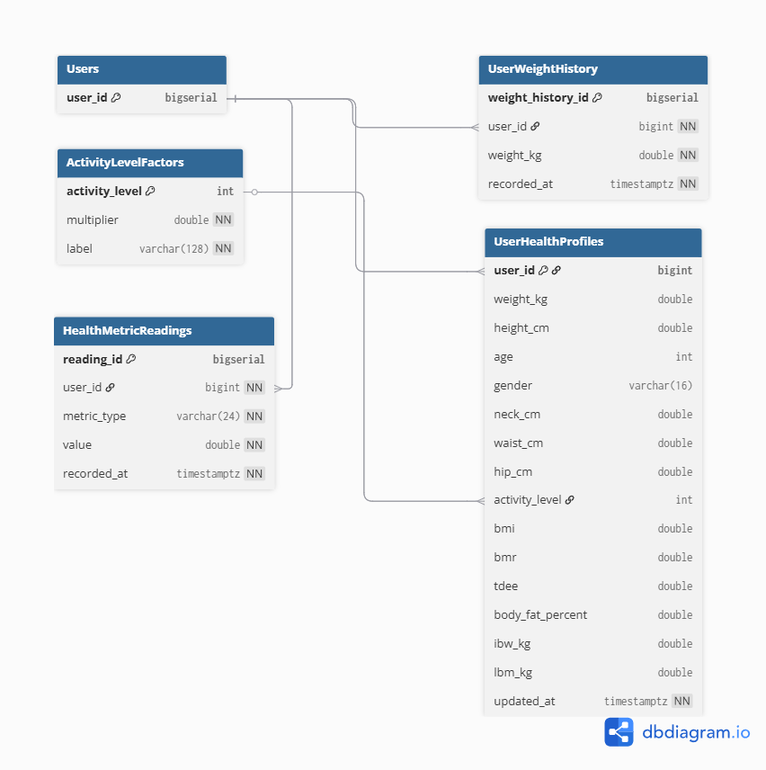
\includegraphics[width=0.85\textwidth]{Images/IMG/ERD/ERDCongcutinhtoan.png}
    \vspace{1em}
    \caption{ERD nhóm tính năng Công cụ tính toán}
    \label{fig:erd_congcu}
\end{figure}

\textbf{Các collection chính và chức năng:}
\begin{itemize}
    \item \textbf{user\_health\_profiles:} Lưu trữ hồ sơ sức khỏe tổng hợp của người dùng gồm cân nặng, chiều cao, tuổi, giới tính, các số đo vòng cơ thể và mức độ vận động. Hệ thống tự động tính toán và lưu kết quả BMI, BMR, TDEE, tỷ lệ mỡ cơ thể và cân nặng lý tưởng.
    \item \textbf{health\_metric\_readings:} Ghi nhận lịch sử chuỗi giá trị các chỉ số sức khỏe theo thời gian, phục vụ vẽ biểu đồ xu hướng và phân tích tiến triển sức khỏe.
    \item \textbf{user\_weight\_history:} Lưu lịch sử cân nặng định kỳ, phục vụ theo dõi tiến độ mục tiêu thay đổi cân nặng theo ngày/tuần/tháng.
    \item \textbf{activity\_level\_factors:} Bảng tra cứu hệ số nhân theo mức độ vận động thể chất (ít vận động, vận động nhẹ, vừa phải, cường độ cao...), được dùng trong công thức tính TDEE.
\end{itemize}

% ─── 7. BẠN BÈ ─────────────────────────────────────────────────────────────────
\subsubsection{Nhóm tính năng Bạn bè}
\label{subsubsec:module_banbe}

Nhóm này kiến tạo và duy trì mạng lưới quan hệ xã hội (Social Graph) giữa các thành viên. Dữ liệu theo dõi được sử dụng để lọc bảng tin, gợi ý kết bạn và hiển thị hoạt động của người trong mạng lưới.

\begin{figure}[H]
    \centering
    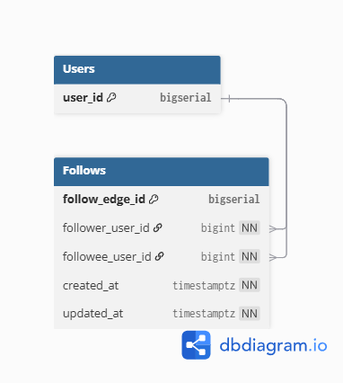
\includegraphics[width=0.55\textwidth]{Images/IMG/ERD/ERDBanbe.png}
    \vspace{1em}
    \caption{ERD nhóm tính năng Bạn bè}
    \label{fig:erd_banbe}
\end{figure}

\textbf{Các collection chính và chức năng:}
\begin{itemize}
    \item \textbf{follows:} Quản lý quan hệ theo dõi một chiều giữa người dùng (người theo dõi và người được theo dõi). Thiết kế dạng cạnh đồ thị cho phép truy vấn hiệu quả danh sách người theo dõi và được theo dõi, phục vụ phân phối bài viết ưu tiên từ mạng lưới bạn bè trên bảng tin.
\end{itemize}

% ─── 8. LỊCH CÁ NHÂN VÀ THÔNG BÁO ───────────────────────────────────────────
\subsubsection{Nhóm tính năng Lịch cá nhân và Thông báo}
\label{subsubsec:module_lichcanhan}

Nhóm này đóng vai trò điều phối dòng thời gian cá nhân, tổng hợp tất cả các mốc lịch từ sự kiện thể thao, thử thách và lịch tập luyện vào một giao diện thống nhất, đồng thời phân phối thông báo thời gian thực đến người dùng.

\begin{figure}[H]
    \centering
    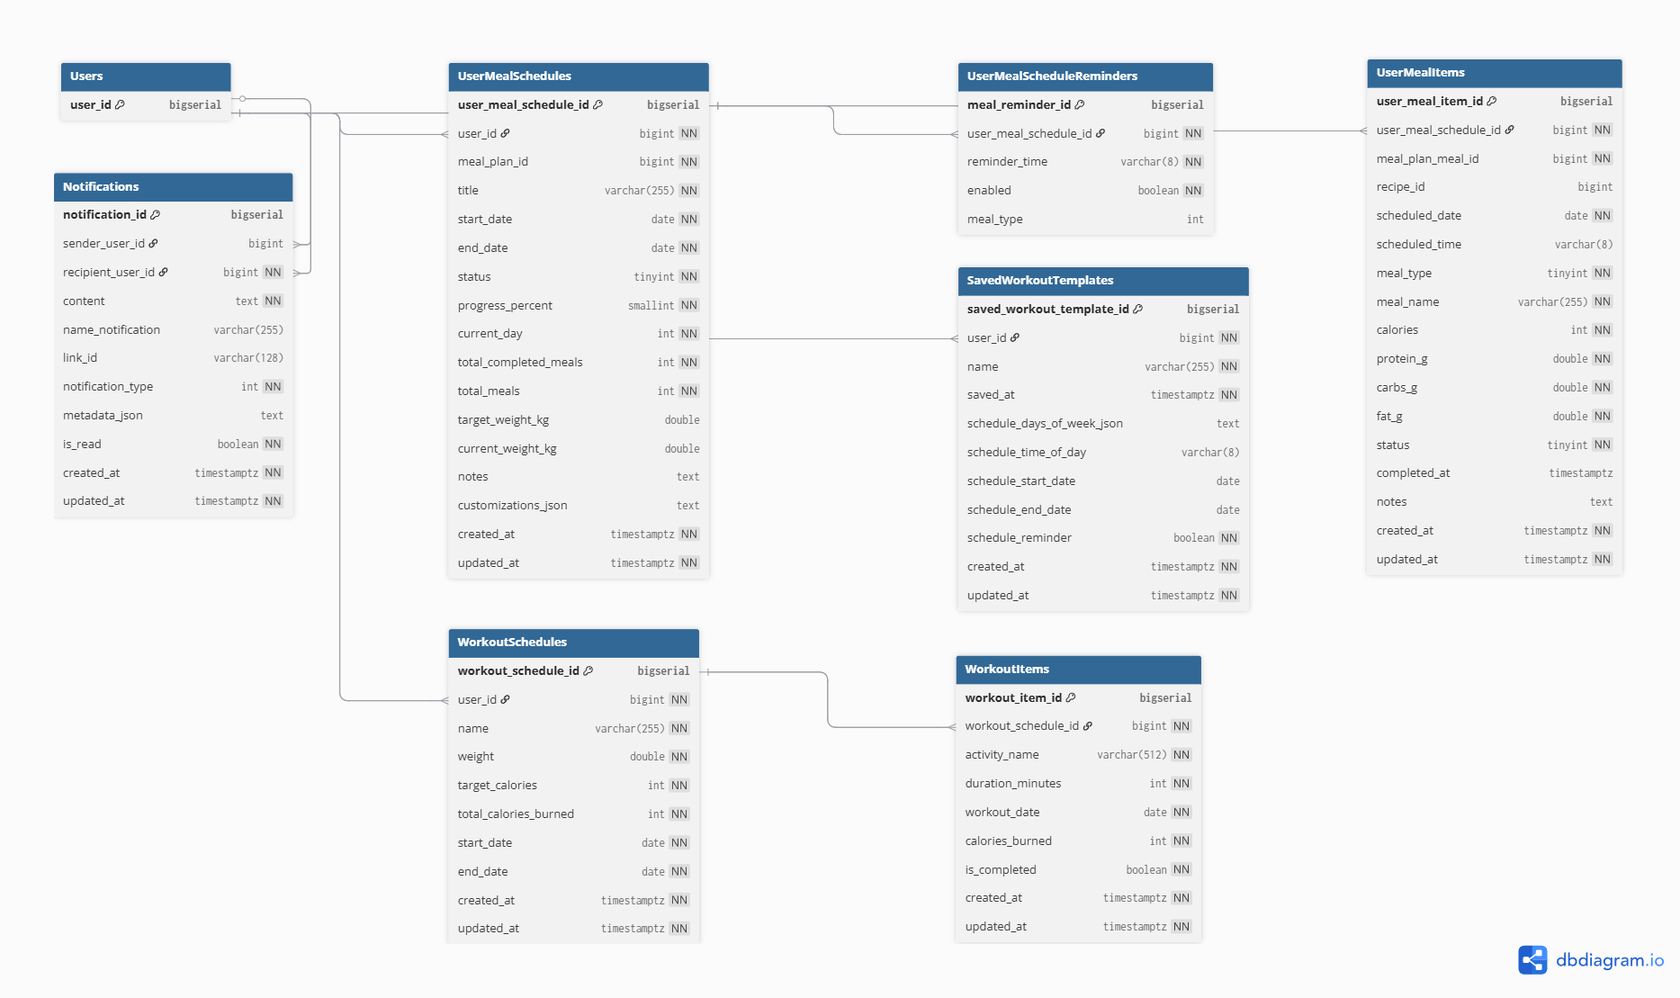
\includegraphics[width=1\textwidth]{Images/IMG/ERD/ERDLichcannhanthongbao.png}
    \vspace{1em}
    \caption{ERD nhóm tính năng Lịch cá nhân và Thông báo}
    \label{fig:erd_lichcanhan}
\end{figure}

\textbf{Các collection chính và chức năng:}
\begin{itemize}
    \item \textbf{notifications:} Lưu trữ và phân phối thông báo đến người nhận, bao gồm người gửi, người nhận, loại thông báo, nội dung, đường dẫn điều hướng, dữ liệu metadata đính kèm và trạng thái đã đọc.
    \item \textbf{workout\_schedules / workout\_items:} Lưu lịch tập luyện cá nhân theo tuần và chi tiết từng hoạt động tập luyện theo ngày cụ thể. Được tổng hợp vào giao diện Calendar để hiển thị và đánh dấu hoàn thành.
    \item \textbf{saved\_workout\_templates:} Giáo án mẫu có lịch lặp lại tự động theo ngày trong tuần và khung giờ cụ thể, hỗ trợ gửi nhắc nhở tích hợp vào Calendar.
    \item \textbf{user\_meal\_schedules:} Lưu kế hoạch thực đơn cá nhân theo ngày, theo dõi tiến độ hoàn thành và số bữa ăn đã thực hiện trong ngày.
    \item \textbf{user\_meal\_schedule\_reminders:} Cấu hình nhắc nhở bữa ăn theo giờ và loại bữa (sáng, trưa, tối, phụ), có thể bật/tắt linh hoạt.
    \item \textbf{user\_meal\_items:} Chi tiết từng bữa ăn trong kế hoạch thực đơn, lưu tên món, ngày và giờ dự kiến, thông tin dinh dưỡng (calo, đạm, tinh bột, chất béo) và trạng thái hoàn thành.
\end{itemize}

% ─── 9. QUẢN LÝ HỆ THỐNG ADMIN ───────────────────────────────────────────────
\subsubsection{Nhóm tính năng Quản lý hệ thống Admin}
\label{subsubsec:module_admin}

Nhóm này cung cấp bộ công cụ quản trị tập trung dành riêng cho Quản trị viên. Admin có quyền giám sát toàn bộ nội dung người dùng, xử lý vi phạm theo nhiều loại đối tượng, đồng thời quản lý danh mục dùng chung và theo dõi mức sử dụng tính năng AI trên nền tảng.

\begin{figure}[H]
    \centering
    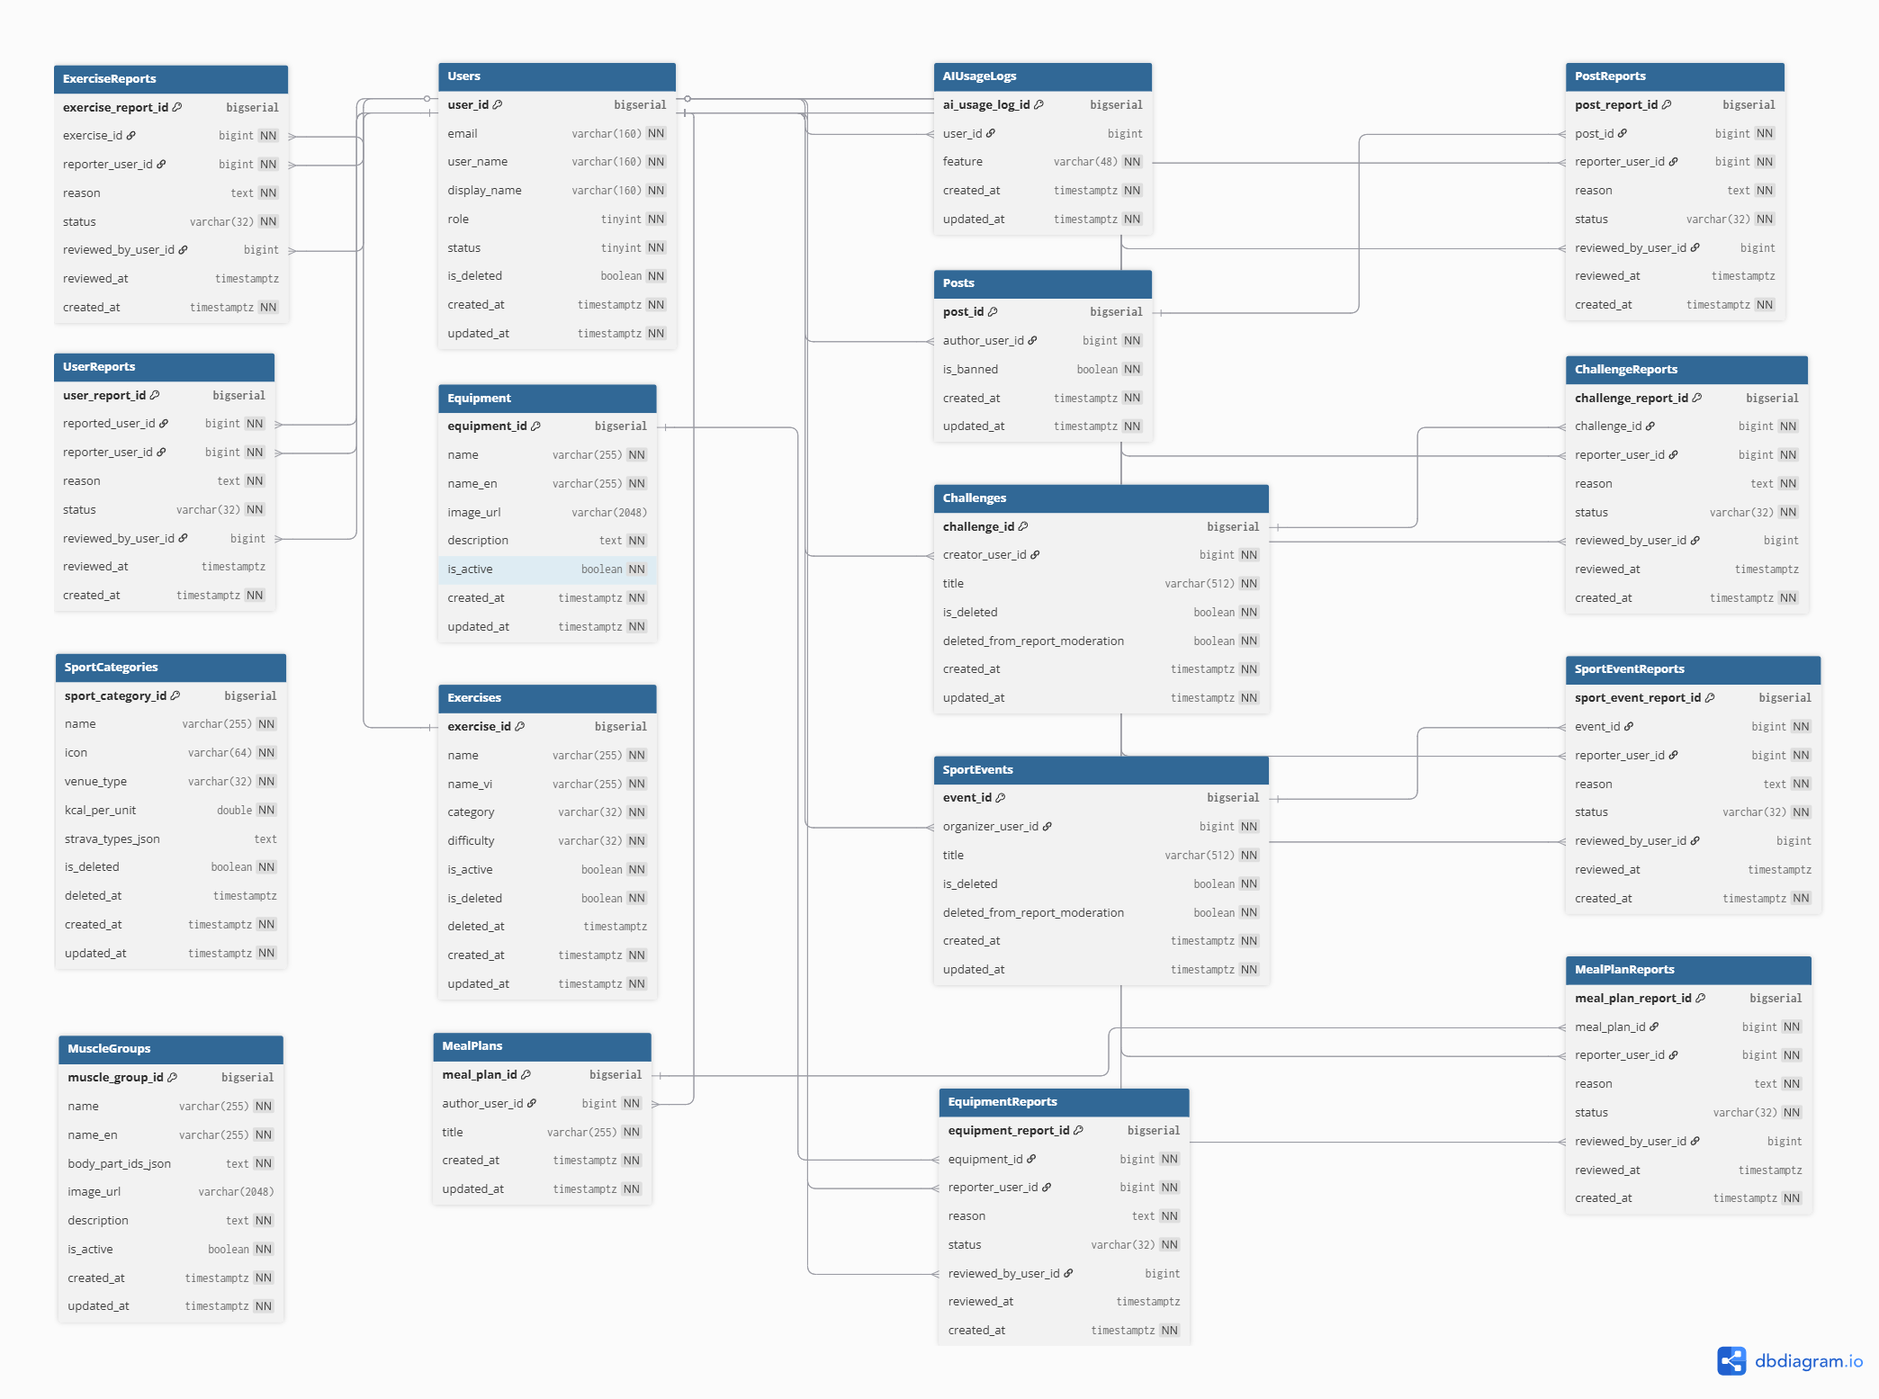
\includegraphics[width=1\textwidth]{Images/IMG/ERD/ERDQuanlyAdmin.png}
    \vspace{1em}
    \caption{ERD nhóm tính năng Quản lý hệ thống Admin}
    \label{fig:erd_admin}
\end{figure}

\textbf{Các collection chính và chức năng:}
\begin{itemize}
    \item \textbf{post\_reports / challenge\_reports / sport\_event\_reports:} Tiếp nhận và quản lý báo cáo vi phạm từ cộng đồng theo từng loại nội dung (bài viết, thử thách, sự kiện thể thao), lưu lý do báo cáo, trạng thái xử lý và thông tin người kiểm duyệt.
    \item \textbf{user\_reports / exercise\_reports:} Cho phép người dùng báo cáo tài khoản vi phạm hoặc bài tập có nội dung sai lệch, phục vụ Admin xem xét và xử lý kịp thời.
    \item \textbf{equipment\_reports / meal\_plan\_reports:} Tiếp nhận báo cáo liên quan đến thiết bị tập luyện và kế hoạch thực đơn không phù hợp.
    \item \textbf{sport\_categories:} Danh mục thể thao do Admin quản lý, lưu tên môn, icon, kiểu địa điểm và lượng calo chuẩn, được dùng làm tiêu chuẩn phân loại sự kiện toàn hệ thống.
    \item \textbf{equipment:} Danh mục thiết bị và dụng cụ tập luyện (tên tiếng Việt, tên tiếng Anh, hình ảnh, trạng thái kích hoạt), phục vụ phân loại và tìm kiếm bài tập.
    \item \textbf{muscle\_groups:} Danh mục nhóm cơ thể với thông tin tên, vị trí trên cơ thể và hình ảnh minh họa, phục vụ phân loại bài tập theo nhóm cơ mục tiêu.
    \item \textbf{meal\_plans:} Quản lý kế hoạch thực đơn mẫu do nhóm quản trị tạo ra, phục vụ gợi ý dinh dưỡng cho người dùng.
    \item \textbf{ai\_usage\_logs:} Ghi nhận nhật ký sử dụng các tính năng AI trên nền tảng (người dùng, tính năng sử dụng, thời điểm), phục vụ phân tích mức độ tiêu thụ và giám sát tài nguyên AI.
\end{itemize}

\section{Thiết kế giao diện}
\label{sec:ui_ux_design}

Thiết kế giao diện hướng đến ba nguyên tắc cốt lõi: dễ sử dụng, nhất quán và hấp dẫn. Mục tiêu là giúp người dùng tiếp cận trực quan và hiệu quả 9 nhóm tính năng chính của nền tảng, bao gồm mạng xã hội cộng đồng, sự kiện thể thao, thử thách, tập luyện, công cụ tính toán sức khỏe, kết nối bạn bè, lịch cá nhân, quản lý tài khoản và phân hệ quản trị Admin.

\subsection{Mục tiêu thiết kế}
\label{subsec:ui_goals}
\begin{itemize}
    \item \textbf{Dễ sử dụng:} Giao diện trực quan, thao tác tối giản và dễ điều hướng cho mọi đối tượng người dùng từ người mới đến người dùng thường xuyên.
    \item \textbf{Nhất quán:} Đồng nhất về bố cục, bảng màu Indigo/Violet, icon và cách hiển thị thông tin trên toàn bộ 9 nhóm tính năng.
    \item \textbf{Responsive:} Hiển thị linh hoạt và tối ưu trên nền tảng Web cho cả desktop và tablet.
    \item \textbf{Hấp dẫn:} Thiết kế hiện đại theo phong cách Glassmorphism, sử dụng hệ màu năng động phù hợp với chủ đề thể dục thể thao và cộng đồng rèn luyện sức khỏe.
    \item \textbf{Phân hệ rõ ràng:} Mỗi nhóm tính năng sở hữu điểm vào (entry point) riêng biệt, đảm bảo người dùng luôn xác định được vị trí và ngữ cảnh sử dụng.
\end{itemize}

\subsection{Prototype và màn hình chính}
\label{subsec:ui_prototype}

\subsubsection{Tổng quan về Prototype}
Trong quá trình thiết kế giao diện người dùng, nhóm phát triển đã xây dựng bộ prototype tương tác hoàn chỉnh nhằm mục đích kiểm tra trải nghiệm người dùng (UX) và thu thập phản hồi trước khi triển khai phát triển chính thức. Prototype được thiết kế sử dụng công cụ MarvelApp\footnote{\href{https://marvelapp.com/prototype/ch16ai1}{Prototype tương tác trên MarvelApp}}, cho phép mô phỏng đầy đủ các tương tác, luồng điều hướng và hành vi của ứng dụng thực tế.

Bộ prototype bao gồm toàn bộ các màn hình chức năng chính của hệ thống, được tổ chức theo 9 nhóm nghiệp vụ cốt lõi như sau:

\begin{itemize}
    \item \textbf{Nhóm Quản lý người dùng:} Màn hình đăng ký, đăng nhập (bao gồm Google OAuth), khôi phục mật khẩu và trang hồ sơ cá nhân tổng hợp.
    \item \textbf{Nhóm Cộng đồng:} Bảng tin Community Feed, đăng bài chia sẻ hoạt động, tương tác Reaction, bình luận phân cấp và kiểm duyệt nội dung bằng AI.
    \item \textbf{Nhóm Sự kiện thể thao:} Khám phá và lọc sự kiện theo phân loại Trong nhà/Ngoài trời, trang chi tiết sự kiện, theo dõi tiến độ GPS, Video Call điểm danh AI và chia sẻ kết quả.
    \item \textbf{Nhóm Thử thách cộng đồng:} Danh sách thử thách, tạo thử thách (thủ công hoặc AI đề xuất), check-in hằng ngày và bảng xếp hạng nội bộ.
    \item \textbf{Nhóm Tập luyện:} Thư viện bài tập lọc theo nhóm cơ/thiết bị, giáo án tập luyện (thủ công hoặc AI gợi ý), tập luyện ngoài trời GPS và lịch sử hoạt động.
    \item \textbf{Nhóm Công cụ tính toán:} Tính toán chỉ số sinh lý học (BMI, BMR, TDEE), phân tích AI và biểu đồ lịch sử chỉ số sức khỏe theo thời gian.
    \item \textbf{Nhóm Bạn bè:} Tìm kiếm và kết nối thành viên, theo dõi (Follow) và quản lý danh sách bạn bè.
    \item \textbf{Nhóm Lịch cá nhân và Thông báo:} Lịch tổng hợp tự động từ sự kiện, thử thách và tập luyện; nhận thông báo thời gian thực.
    \item \textbf{Nhóm Quản lý hệ thống Admin:} Dashboard tăng trưởng, quản lý người dùng và nội dung, kiểm duyệt báo cáo vi phạm, cấu hình danh mục thể thao.
\end{itemize}

\subsubsection{Các màn hình chính}

% ─── 1. QUẢN LÝ NGƯỜI DÙNG ───────────────────────────────────────────────────
\paragraph{Nhóm tính năng Quản lý người dùng}
Phân hệ quản lý người dùng là điểm khởi đầu bắt buộc để mỗi cá nhân xác lập danh tính số trên nền tảng FitConnect. Màn hình đăng nhập và đăng ký được thiết kế tối giản với biểu mẫu rõ ràng, hỗ trợ đăng nhập qua Google OAuth 2.0 song song với xác thực Email truyền thống. Hệ thống tích hợp luồng cấp phát lại mật khẩu (Forgot Password) hoàn toàn tự động qua Email. Sau khi đăng nhập, trang hồ sơ cá nhân (Profile) tập hợp toàn bộ thống kê hoạt động của người dùng bao gồm danh sách bài viết đã chia sẻ, thành tích sự kiện, thử thách đang tham gia và lịch tập luyện.

\begin{figure}[H]
    \centering
    
\includegraphics[width=0.85\textwidth]{Images/IMG/TaiKhoan/dangky.jpg}
    \vspace{1em}
    \caption{(a) Đăng ký tài khoản}
    \label{fig:ui_dangky}
\end{figure}

\begin{figure}[H]
    \centering
    
\includegraphics[width=0.85\textwidth]{Images/IMG/TaiKhoan/quenmatkhau.jpg}
    \vspace{1em}
    \caption{(b) Quên mật khẩu}
    \label{fig:ui_quenmatkhau}
\end{figure}

\begin{figure}[H]
    \centering
    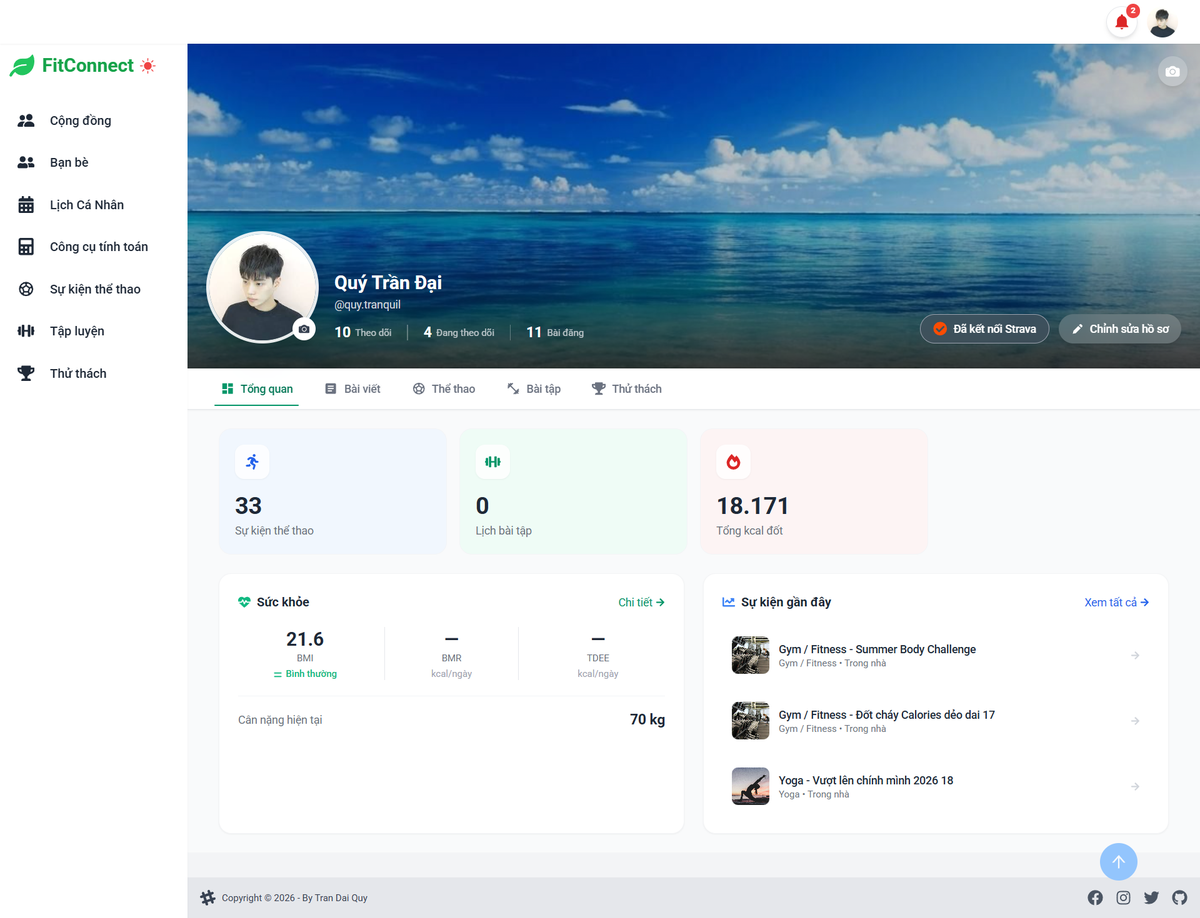
\includegraphics[width=0.85\textwidth]{Images/IMG/TaiKhoan/canhan.jpg}
    \vspace{1em}
    \caption{(c) Màn hình hồ sơ cá nhân}
    \label{fig:ui_canhan}
\end{figure}

% ─── 2. CỘNG ĐỒNG ─────────────────────────────────────────────────────────────
\paragraph{Nhóm tính năng Cộng đồng}
Không gian cộng đồng là trung tâm tương tác xã hội của nền tảng. Bảng tin (Community Feed) liên tục cập nhật bài đăng từ mạng lưới bạn bè theo thứ tự thời gian thực, hỗ trợ tương tác Reaction, bình luận phân cấp và chia sẻ bài đăng. Người dùng có thể tạo bài viết đính kèm hình ảnh; hệ thống tích hợp mô-đun AI kiểm duyệt tự động nhằm phát hiện và từ chối các hình ảnh nhạy cảm trước khi hiển thị.

\begin{figure}[H]
    \centering
    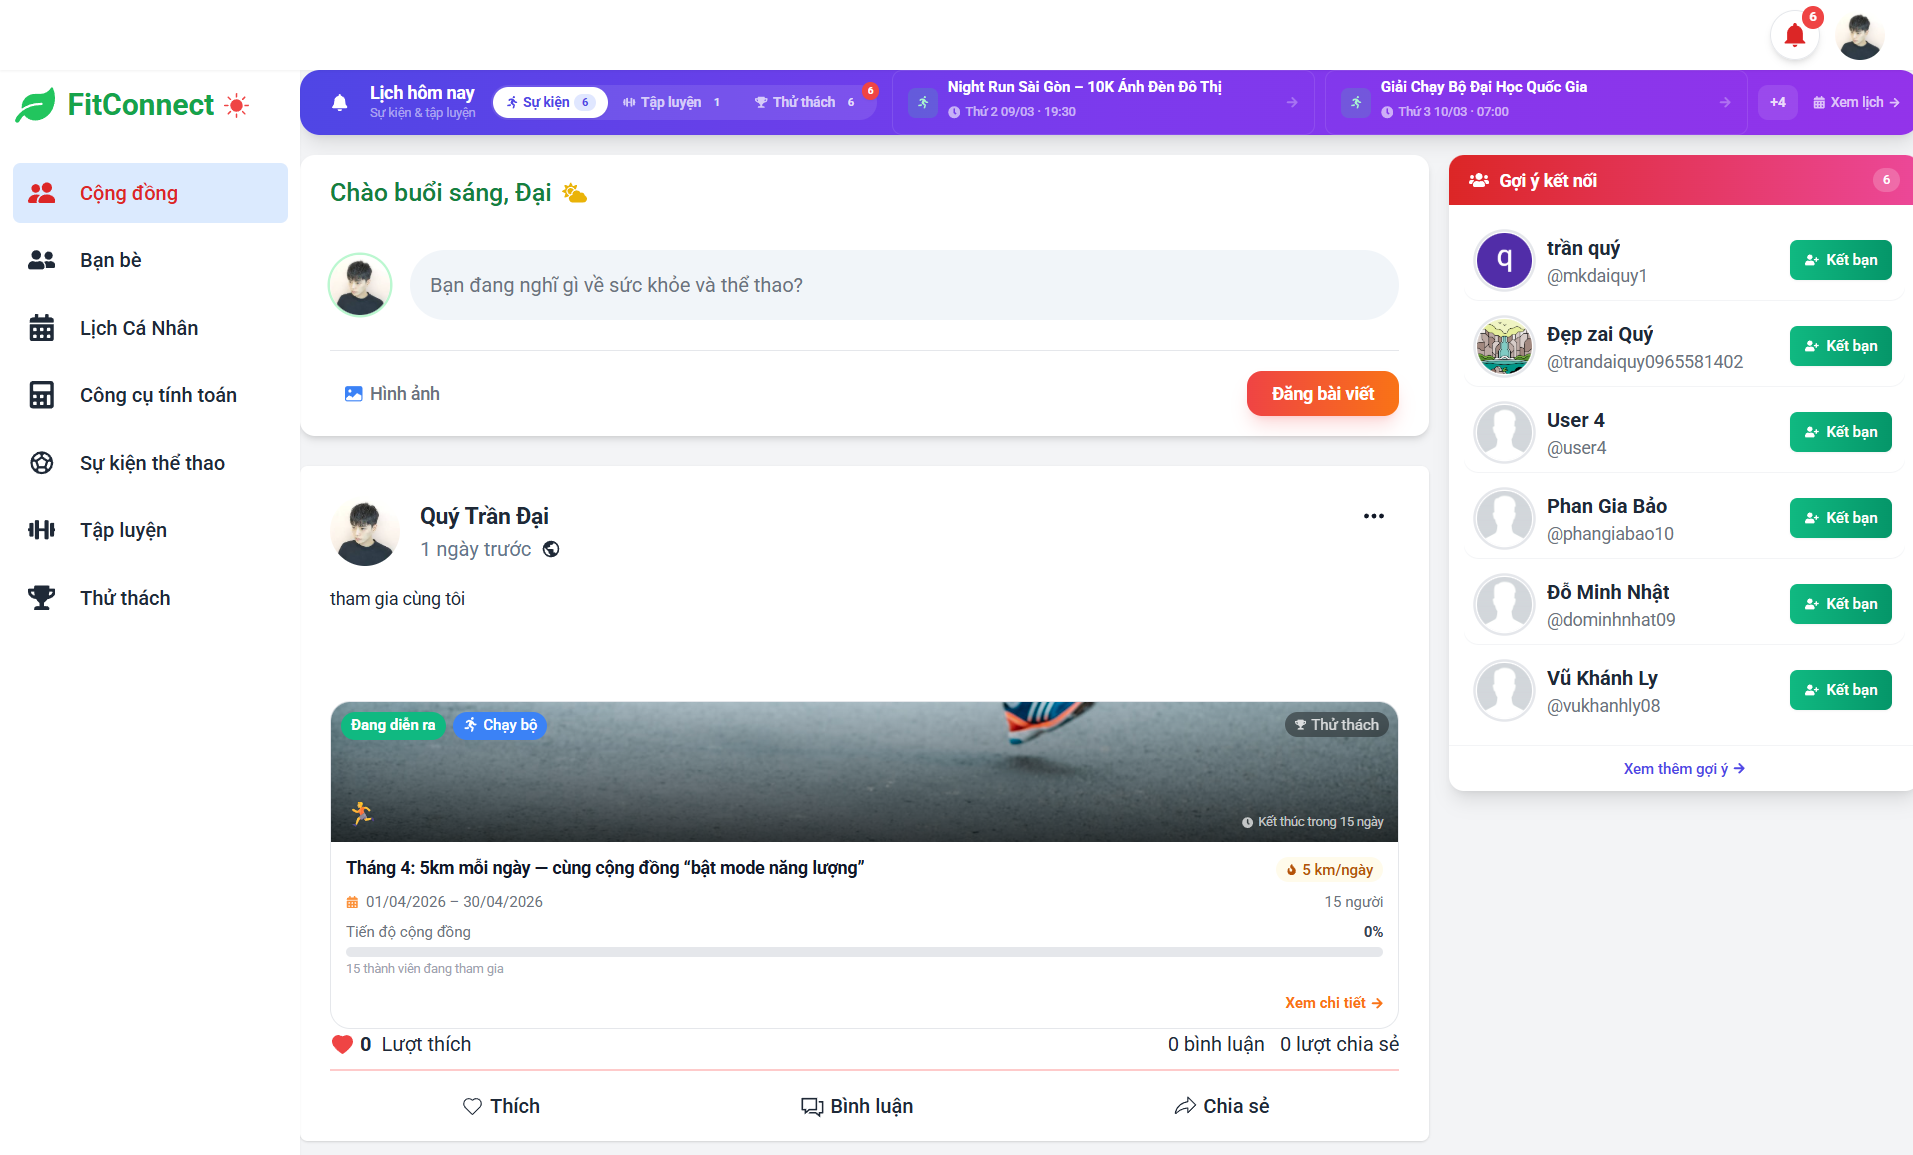
\includegraphics[width=0.85\textwidth]{Images/IMG/CongDong/congdong.jpg}
    \vspace{1em}
    \caption{(a) Bảng tin cộng đồng}
    \label{fig:ui_congdong_feed}
\end{figure}

\begin{figure}[H]
    \centering
    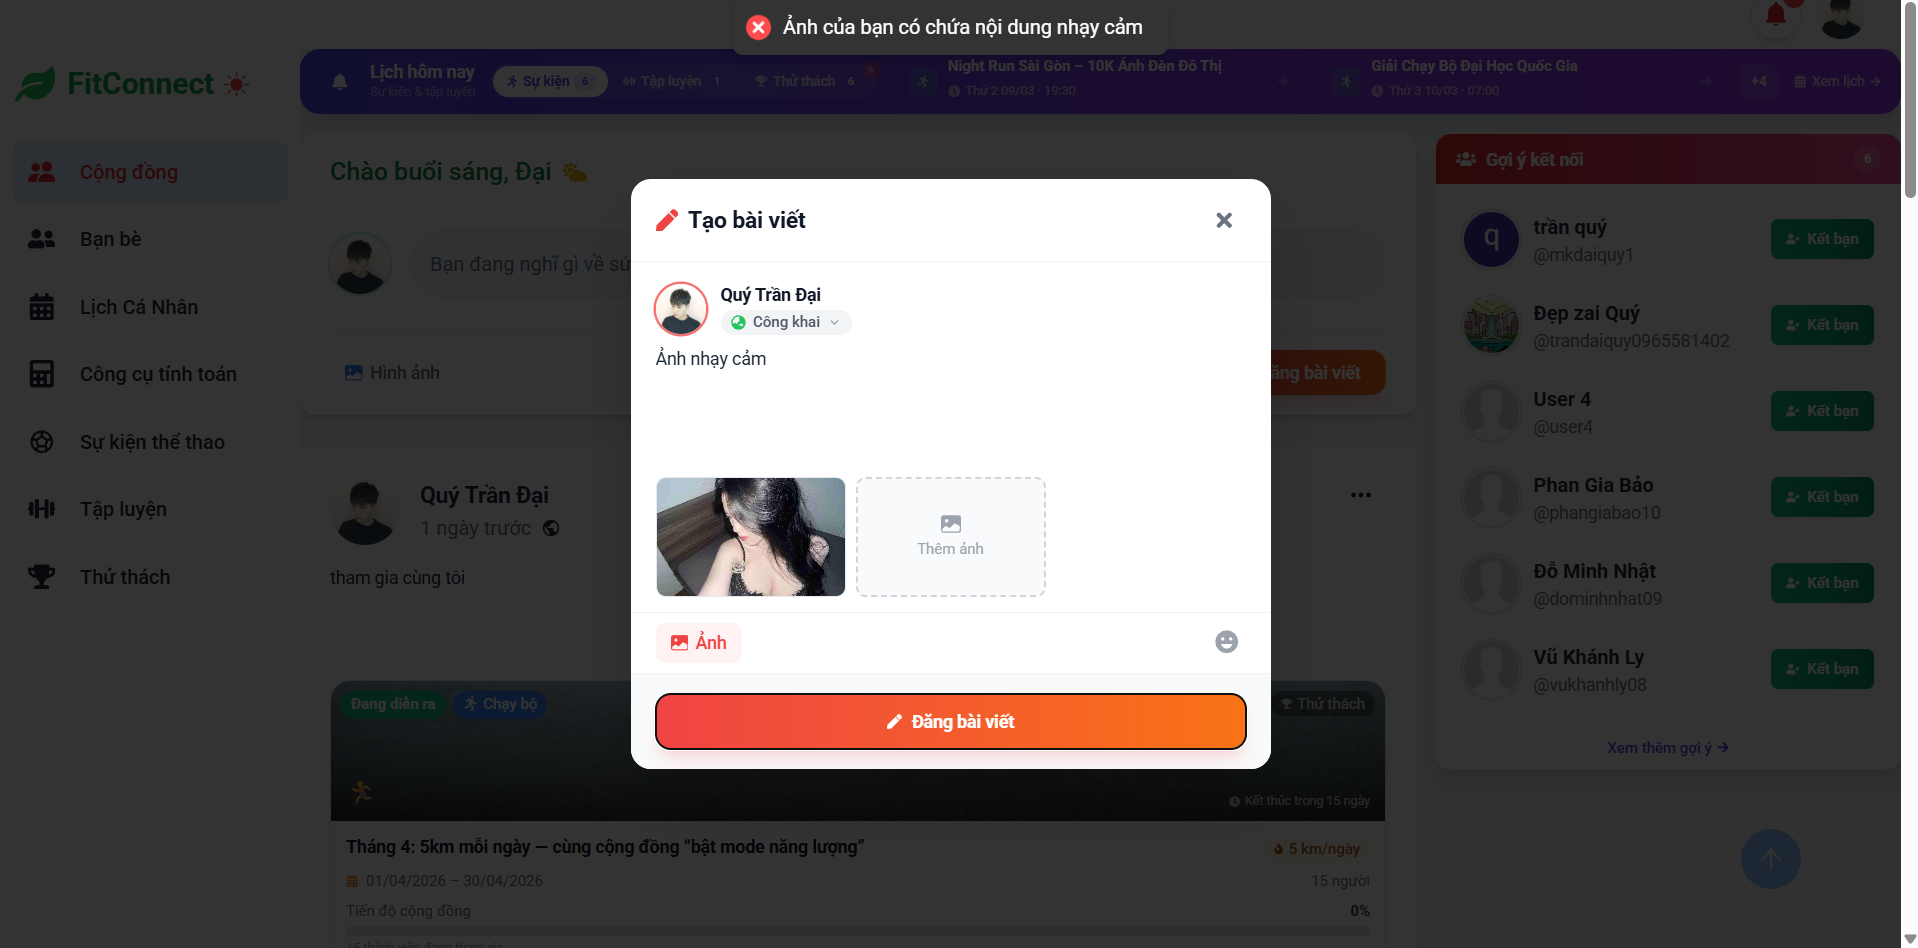
\includegraphics[width=0.85\textwidth]{Images/IMG/CongDong/AInhanbietanhnhaycam.jpg}
    \vspace{1em}
    \caption{(b) AI phát hiện và từ chối hình ảnh nhạy cảm}
    \label{fig:ui_congdong_ai}
\end{figure}

% ─── 3. SỰ KIỆN THỂ THAO ──────────────────────────────────────────────────────
\paragraph{Nhóm tính năng Sự kiện thể thao}
Phân hệ Sự kiện thể thao hỗ trợ người dùng tạo, tham gia và theo dõi các sự kiện thi đua cộng đồng. Màn hình khám phá hiển thị danh sách sự kiện dạng thẻ với bộ lọc phân loại Trong nhà/Ngoài trời. Tại trang chi tiết sự kiện, người dùng xem được danh sách người tham gia và tiến trình tổng thể. Đối với sự kiện Ngoài trời, hệ thống ghi nhận lộ trình GPS thời gian thực. Đối với sự kiện Trong nhà, giao diện Video Call nhóm được tích hợp với mô-đun AI nhận diện khuôn mặt để tự động xác nhận thời gian hiện diện của từng thành viên.

\begin{figure}[H]
    \centering
    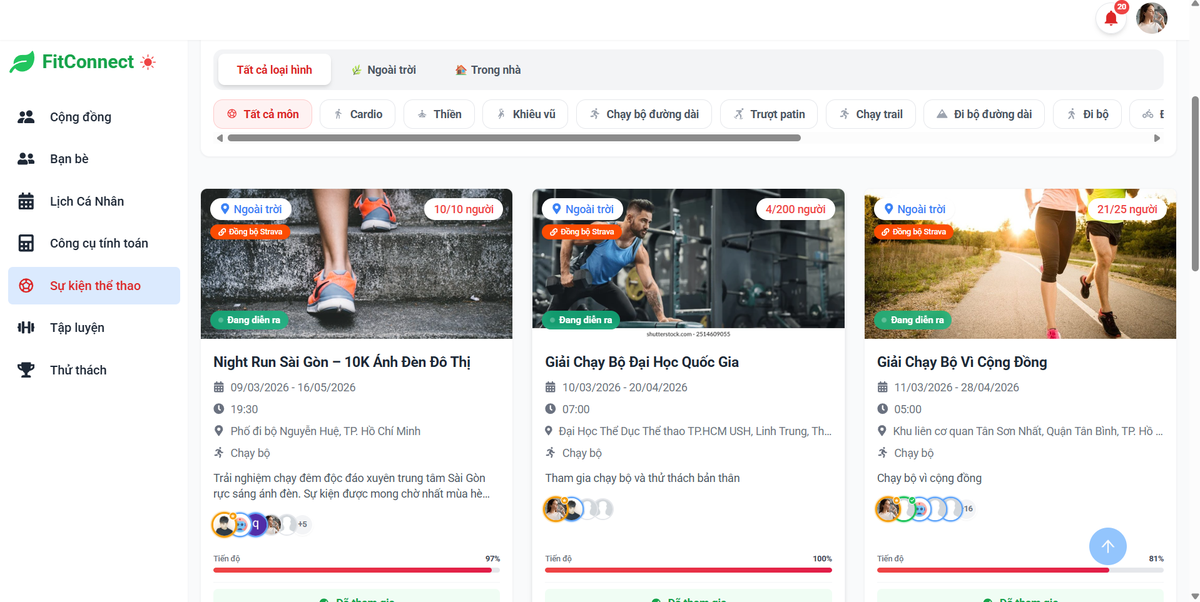
\includegraphics[width=0.85\textwidth]{Images/IMG/Sukienthethao/sukienthethao1.jpg}
    \vspace{1em}
    \caption{(a) Quản lý sự kiện thể thao}
    \label{fig:ui_quanlisukien}
\end{figure}

\begin{figure}[H]
    \centering
    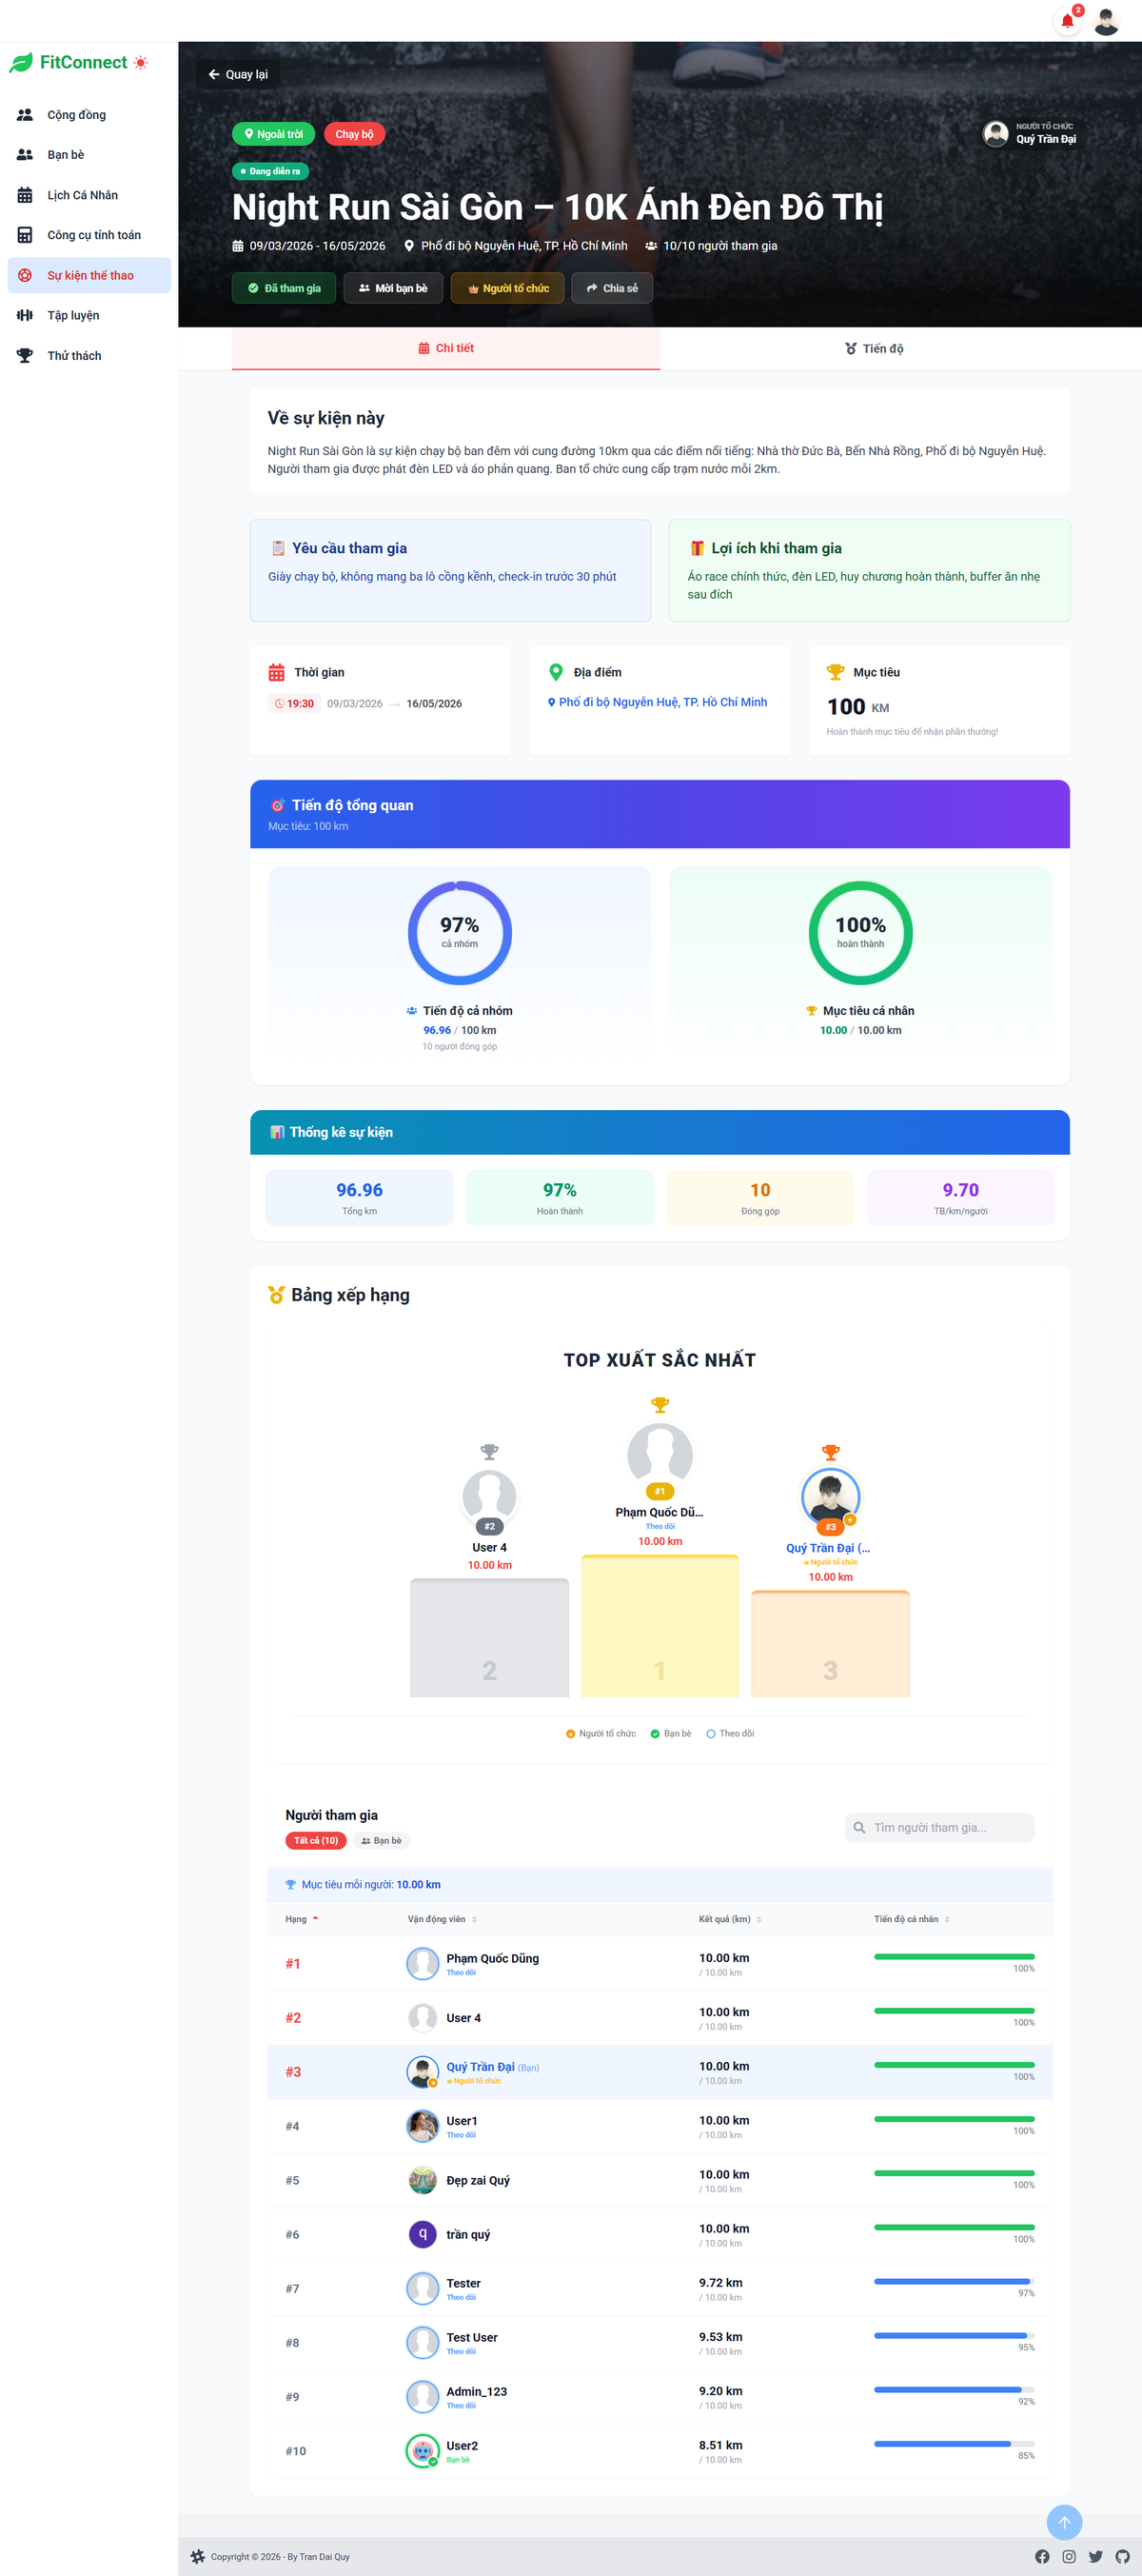
\includegraphics[width=0.85\textwidth]{Images/IMG/Sukienthethao/chitietsukien.jpg}
    \vspace{1em}
    \caption{(b) Chi tiết sự kiện và danh sách người tham gia}
    \label{fig:ui_chitietsukien}
\end{figure}

\begin{figure}[H]
    \centering
    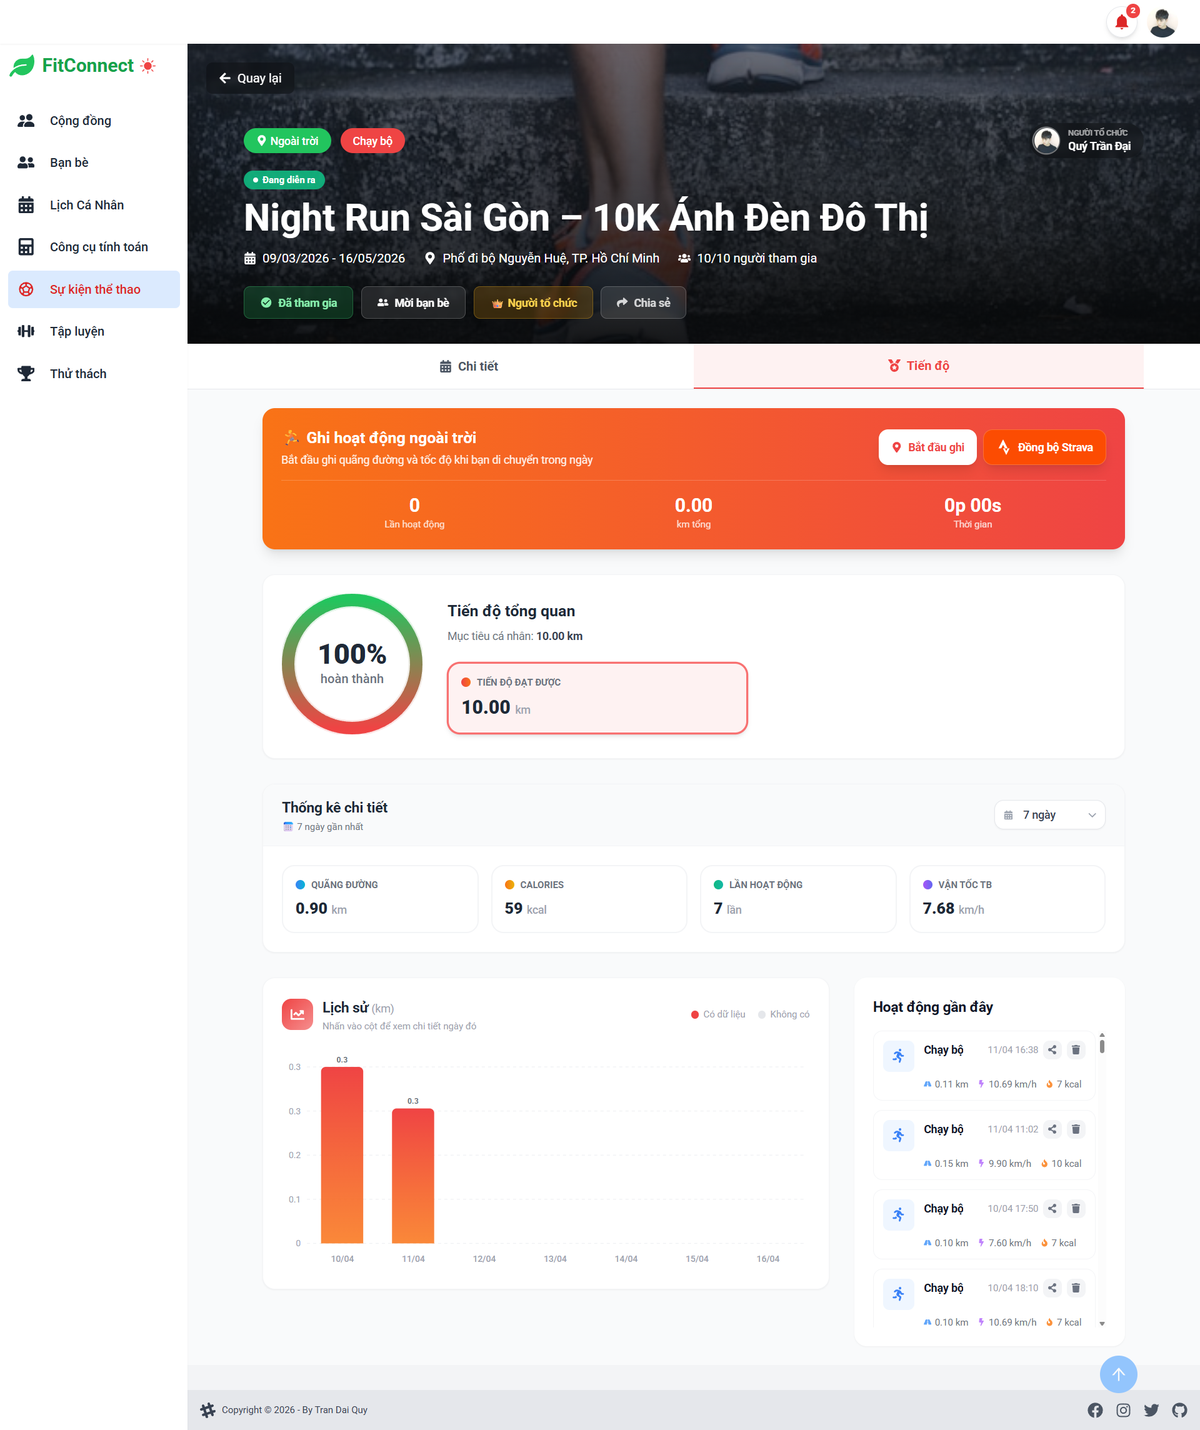
\includegraphics[width=0.85\textwidth]{Images/IMG/Sukienthethao/tabtiendosukien.jpg}
    \vspace{1em}
    \caption{(c) Theo dõi tiến độ thi đua sự kiện}
    \label{fig:ui_tiendosukien}
\end{figure}

\begin{figure}[H]
    \centering
    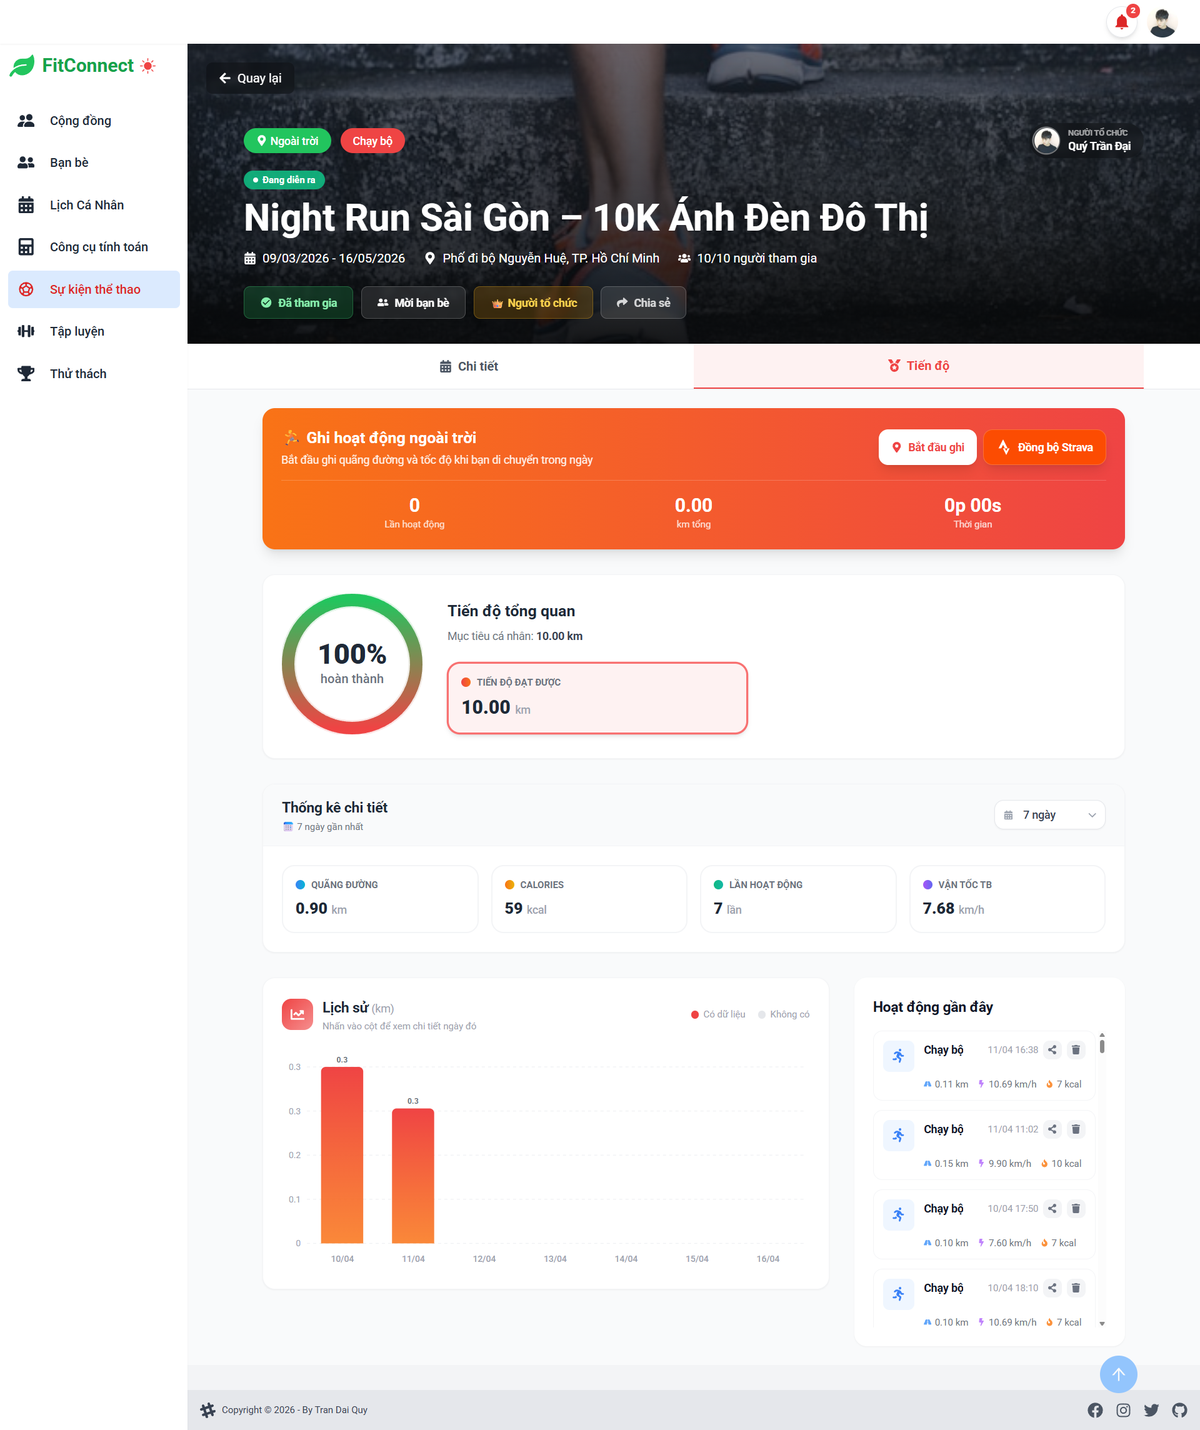
\includegraphics[width=0.85\textwidth]{Images/IMG/Sukienthethao/tabtiendosukien.jpg}
    \vspace{1em}
    \caption{(d) Ghi nhận tiến độ GPS thời gian thực}
    \label{fig:ui_gps_tracking}
\end{figure}

\begin{figure}[H]
    \centering
    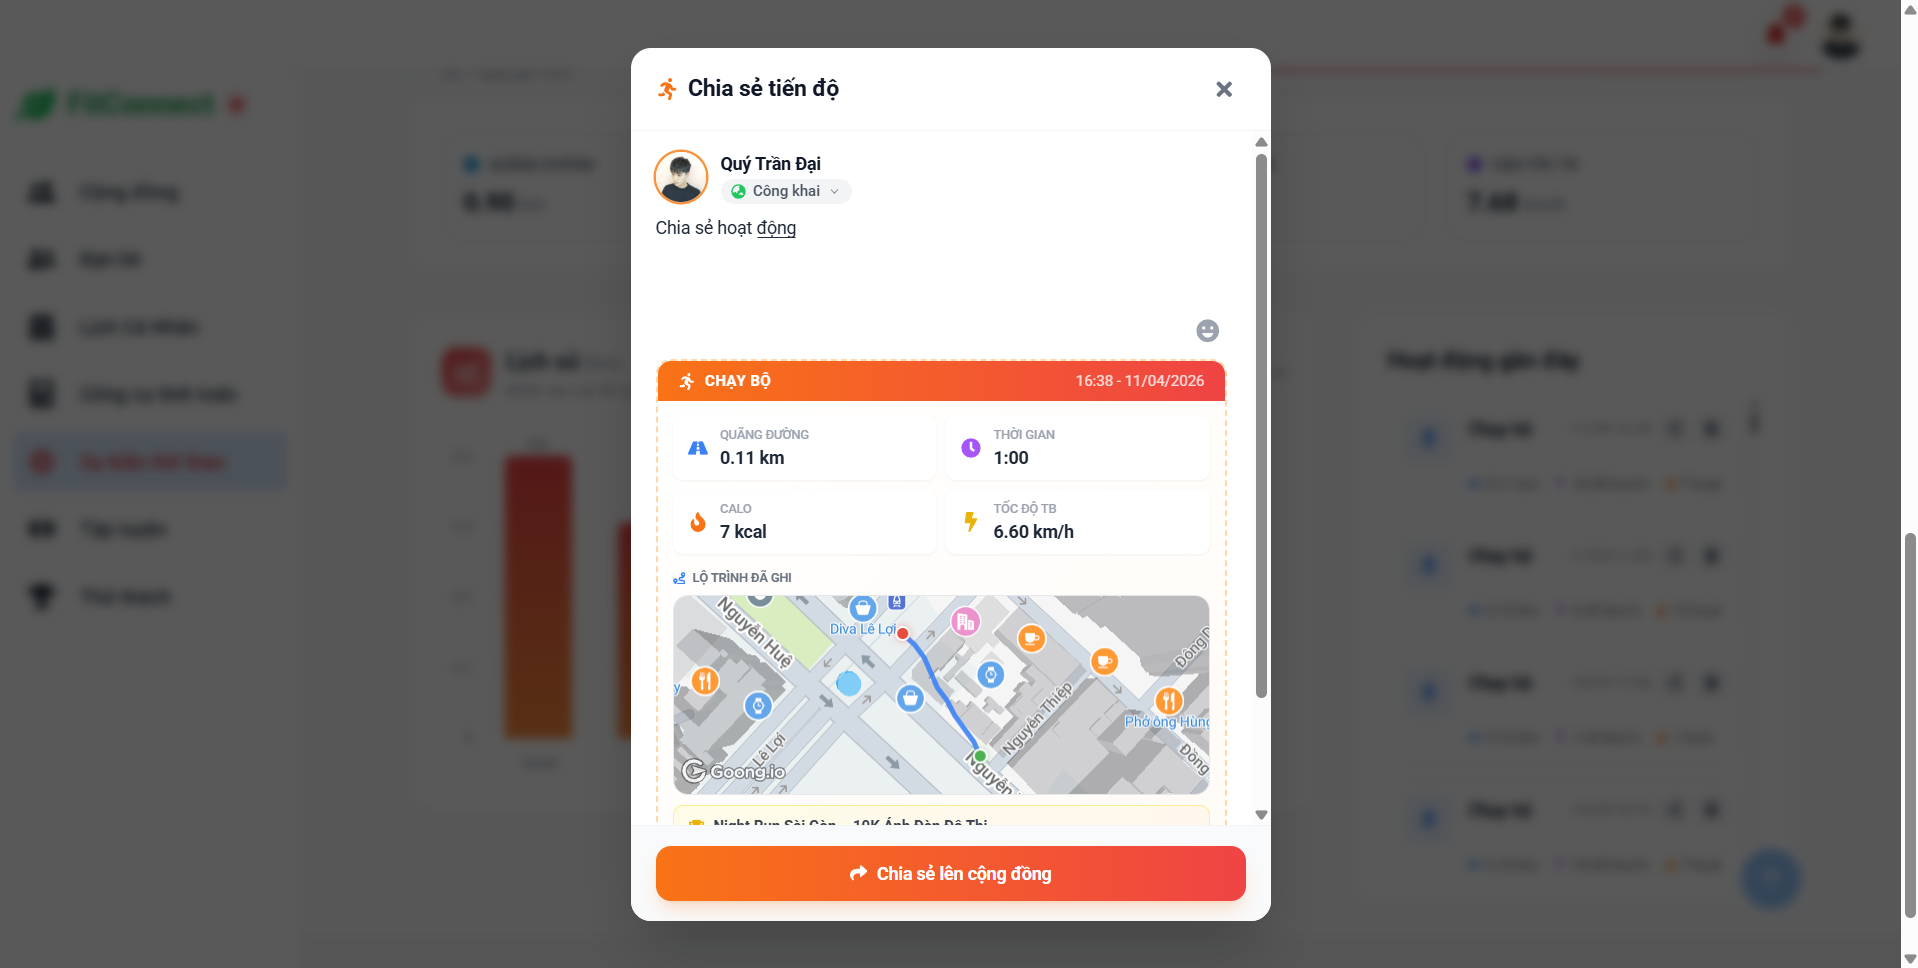
\includegraphics[width=0.85\textwidth]{Images/IMG/Sukienthethao/chiasehoatdong.jpg}
    \vspace{1em}
    \caption{(e) Chia sẻ hoạt động sự kiện lên bảng tin}
    \label{fig:ui_chiasehoatdong}
\end{figure}

\begin{figure}[H]
    \centering
    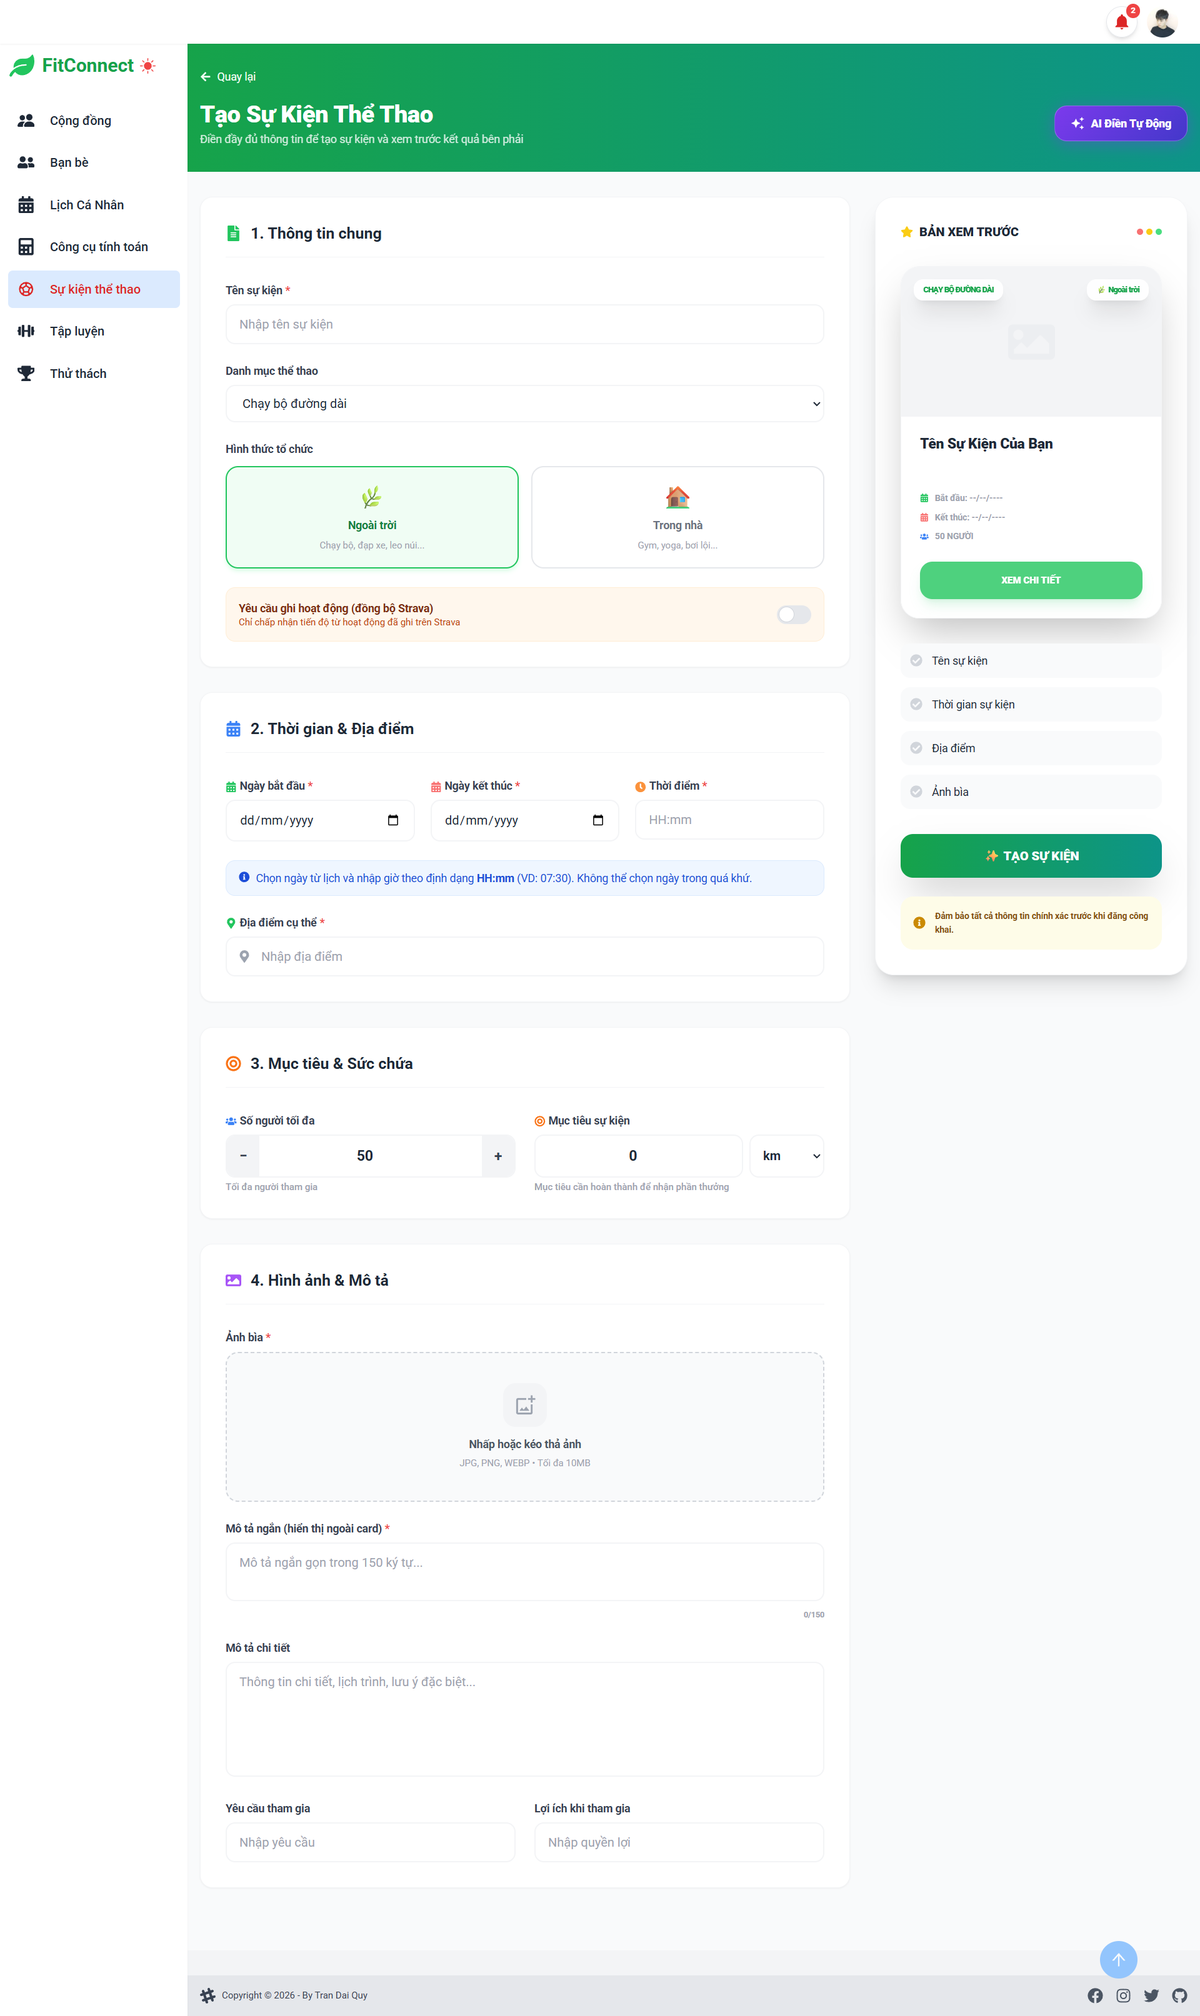
\includegraphics[width=0.85\textwidth]{Images/IMG/Sukienthethao/taosukienmoi.jpg}
    \vspace{1em}
    \caption{(f) Tạo sự kiện mới}
    \label{fig:ui_taosukien}
\end{figure}

% ─── 4. THỬ THÁCH CỘNG ĐỒNG ───────────────────────────────────────────────────
\paragraph{Nhóm tính năng Thử thách cộng đồng}
Thử thách cộng đồng cung cấp không gian rèn luyện kỷ luật theo ngày. Người dùng có thể tự tạo thử thách thuộc các hạng mục khác nhau hoặc để AI tự động gợi ý kịch bản thử thách. Mỗi ngày người tham gia thực hiện check-in theo phương thức tương ứng: chụp ảnh bữa ăn (AI nhận diện), hoàn thành bài tập, hoặc ghi nhận GPS ngoài trời. Giao diện tiến độ thể hiện bảng xếp hạng nội bộ và nhật ký check-in theo ngày của tất cả thành viên.

\begin{figure}[H]
    \centering
    
\includegraphics[width=0.85\textwidth]{Images/IMG/thuthach/danhsachthuthach.jpg}
    \vspace{1em}
    \caption{(a) Danh sách thử thách cộng đồng}
    \label{fig:ui_danhsachthuthach}
\end{figure}

\begin{figure}[H]
    \centering
    
\includegraphics[width=0.85\textwidth]{Images/IMG/thuthach/chitietthuthach.jpg}
    \vspace{1em}
    \caption{(b) Chi tiết thử thách}
    \label{fig:ui_chitietthuthach}
\end{figure}

\begin{figure}[H]
    \centering
    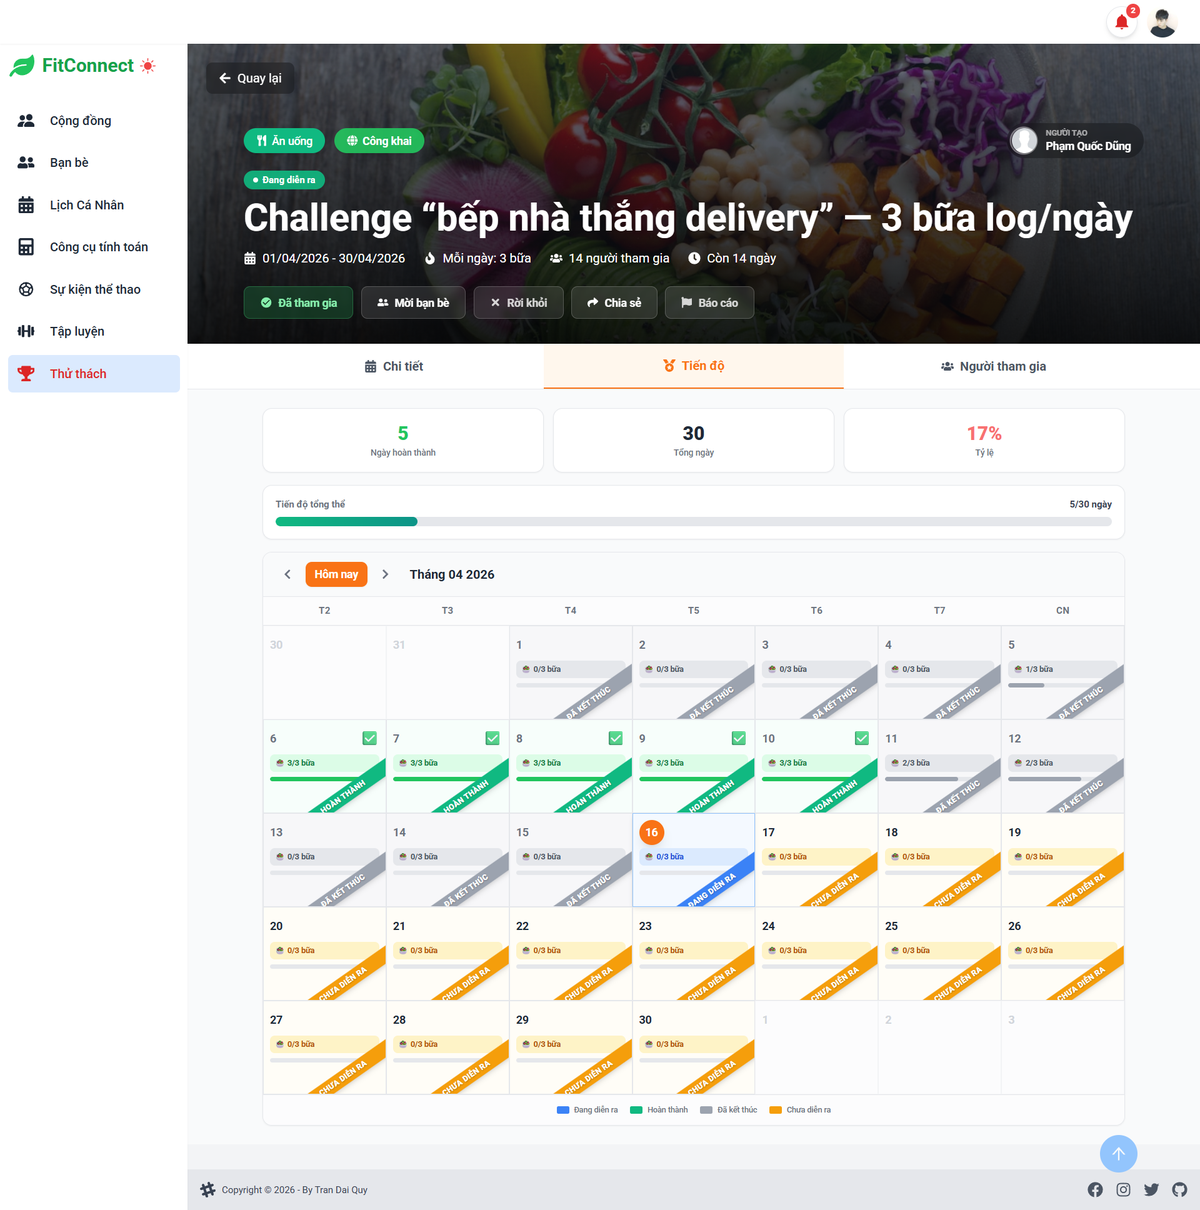
\includegraphics[width=0.85\textwidth]{Images/IMG/thuthach/tiendothuthach.jpg}
    \vspace{1em}
    \caption{(c) Tiến độ và bảng xếp hạng nội bộ}
    \label{fig:ui_tiendothuthach}
\end{figure}

\begin{figure}[H]
    \centering
    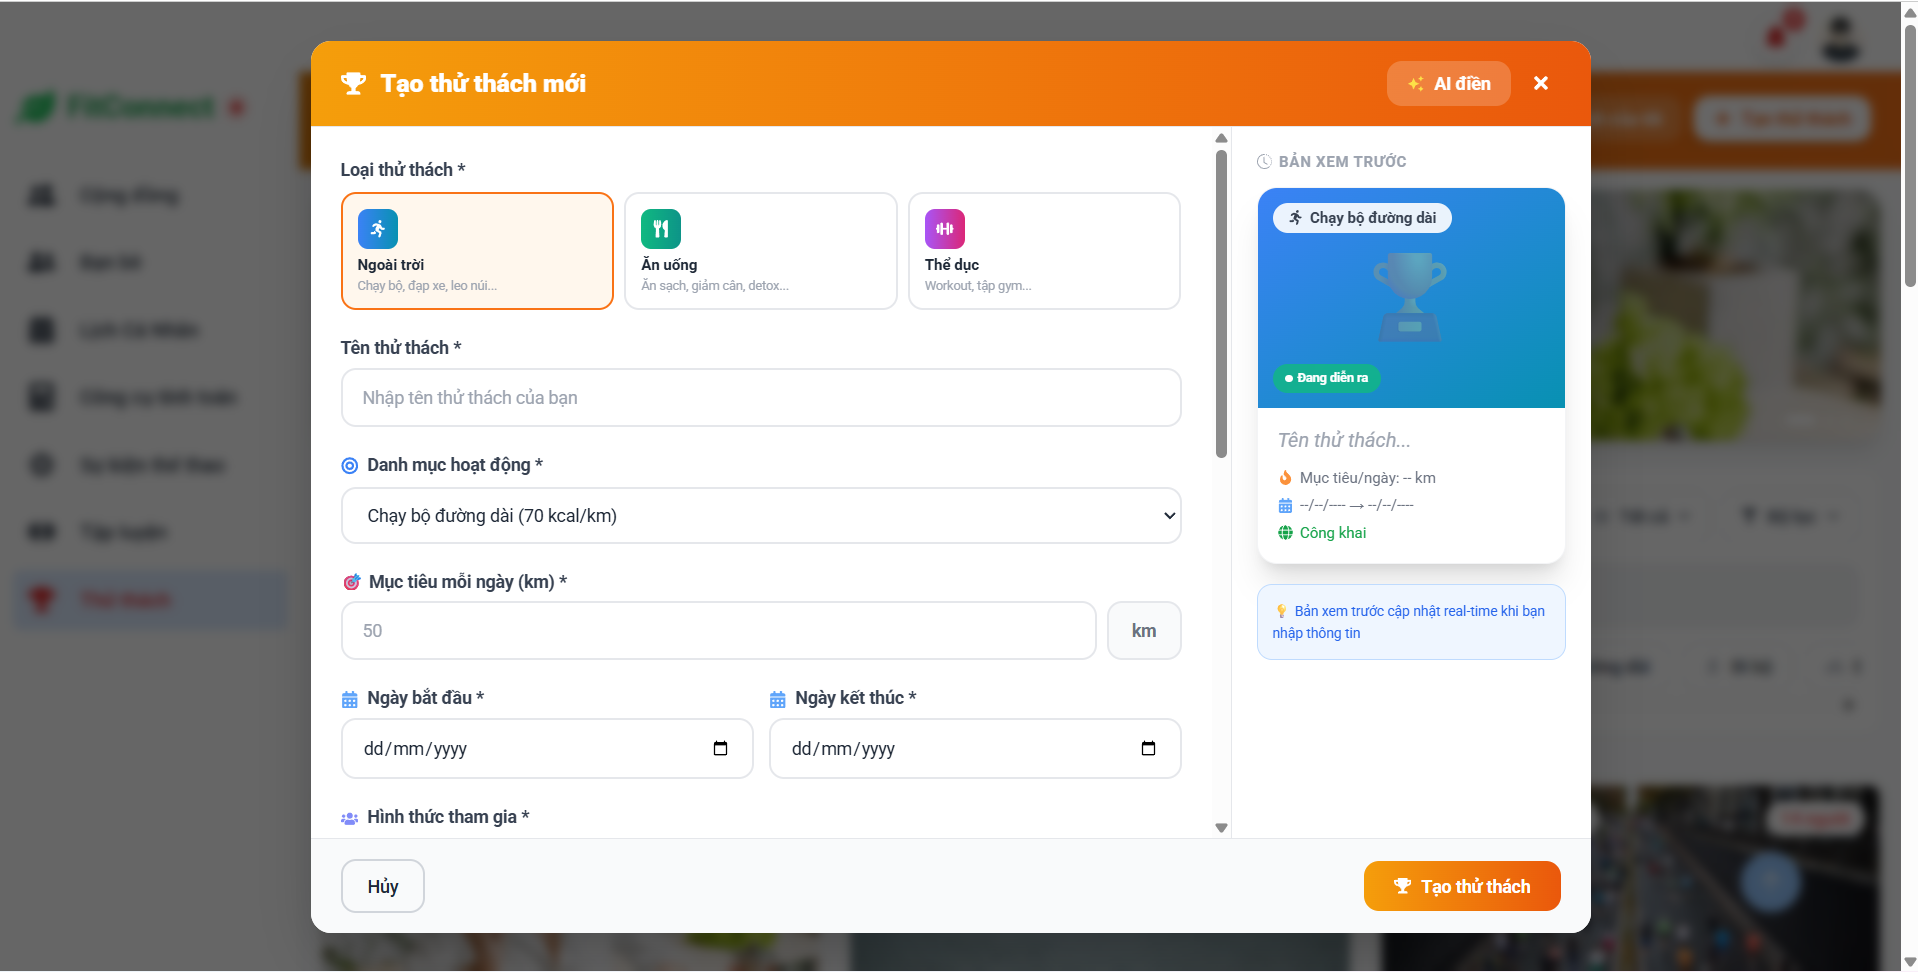
\includegraphics[width=0.85\textwidth]{Images/IMG/thuthach/taothuthach.jpg}
    \vspace{1em}
    \caption{(d) Tạo thử thách mới}
    \label{fig:ui_taothuthach}
\end{figure}

\begin{figure}[H]
    \centering
    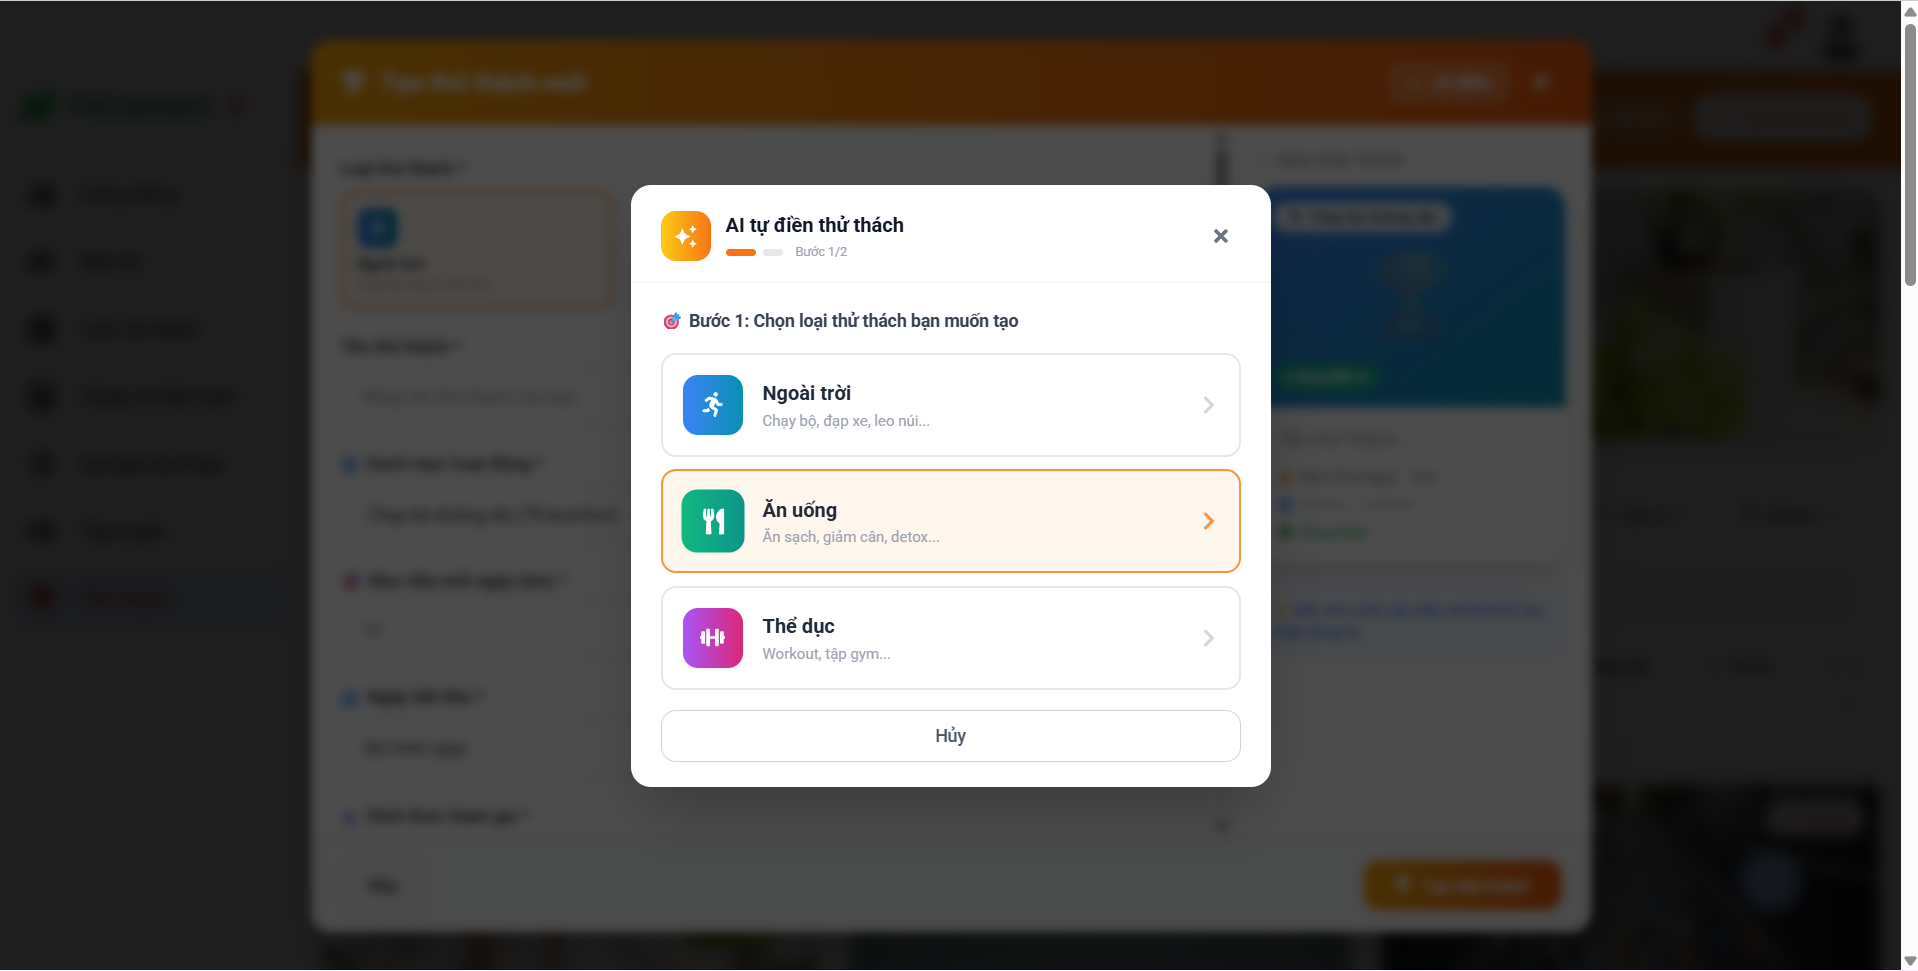
\includegraphics[width=0.85\textwidth]{Images/IMG/thuthach/aidienthuthach1.jpg}
    \vspace{1em}
    \caption{(e) AI tự động đề xuất nội dung thử thách}
    \label{fig:ui_aithuthach}
\end{figure}

\begin{figure}[H]
    \centering
    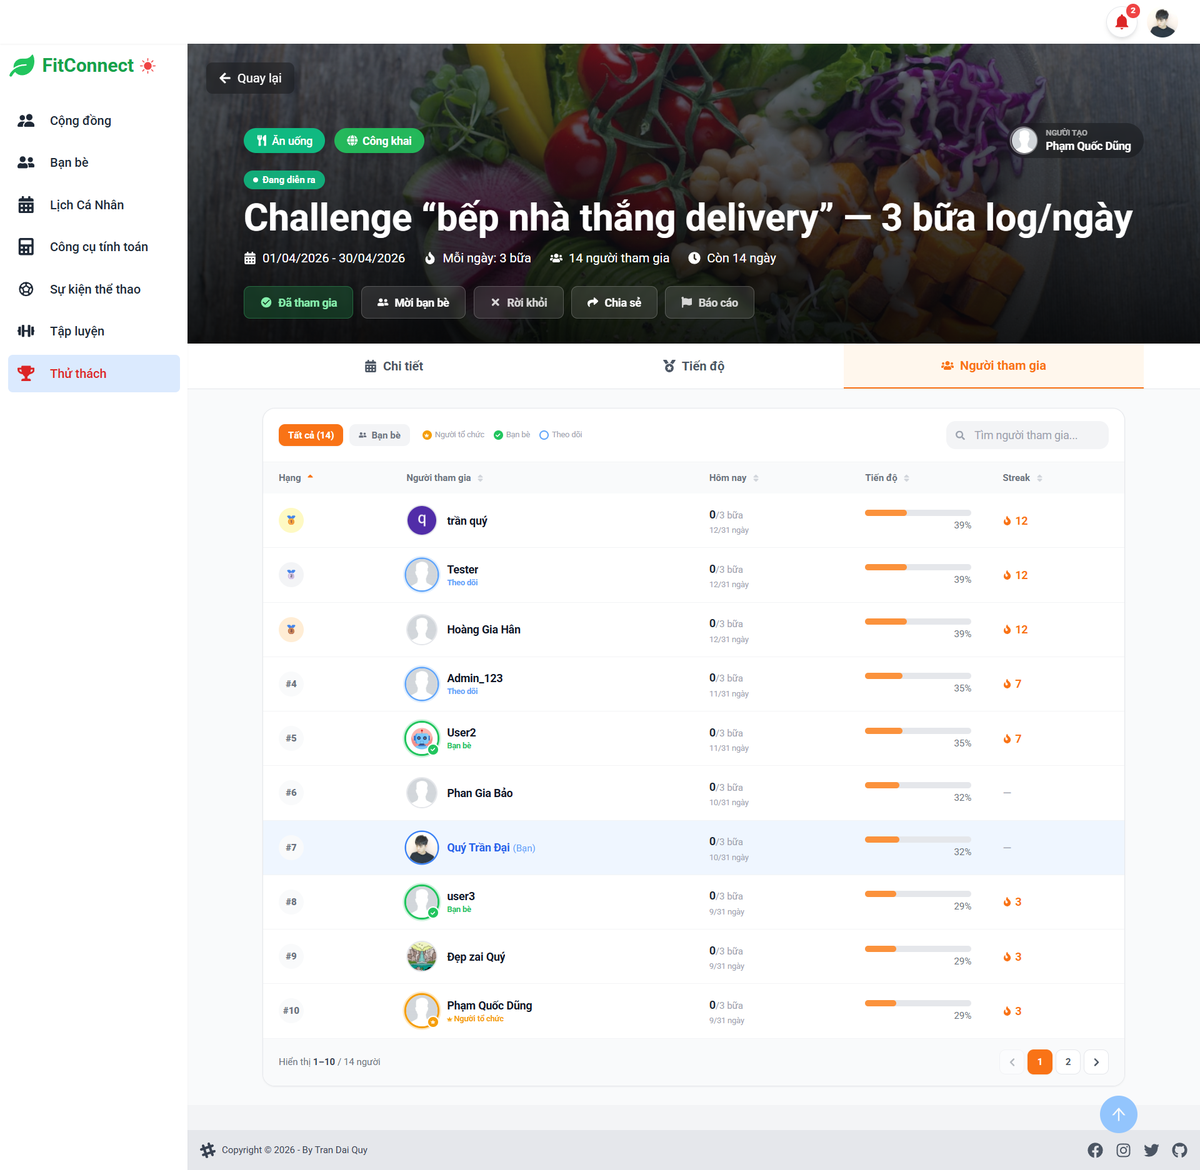
\includegraphics[width=0.85\textwidth]{Images/IMG/thuthach/nguoithamgiathuthach.jpg}
    \vspace{1em}
    \caption{(f) Danh sách người tham gia thử thách}
    \label{fig:ui_nguoithamgiathuthach}
\end{figure}

% ─── 5. TẬP LUYỆN ─────────────────────────────────────────────────────────────
\paragraph{Nhóm tính năng Tập luyện}
Phân hệ Tập luyện cung cấp không gian rèn luyện cá nhân độc lập. Người dùng lọc bài tập theo nhóm cơ mục tiêu hoặc thiết bị dụng cụ, xem video hướng dẫn và tinh chỉnh thông số. Hệ thống tích hợp công cụ AI gợi ý giáo án dựa trên chỉ số sức khỏe và mục tiêu cá nhân. Người dùng có thể lưu giáo án vào lịch tập và thực hiện tập luyện ngoài trời (chạy bộ, đạp xe) với ghi nhận GPS. Màn hình lịch sử tập luyện tổng hợp toàn bộ dữ liệu hoạt động theo thời gian.

\begin{figure}[H]
    \centering
    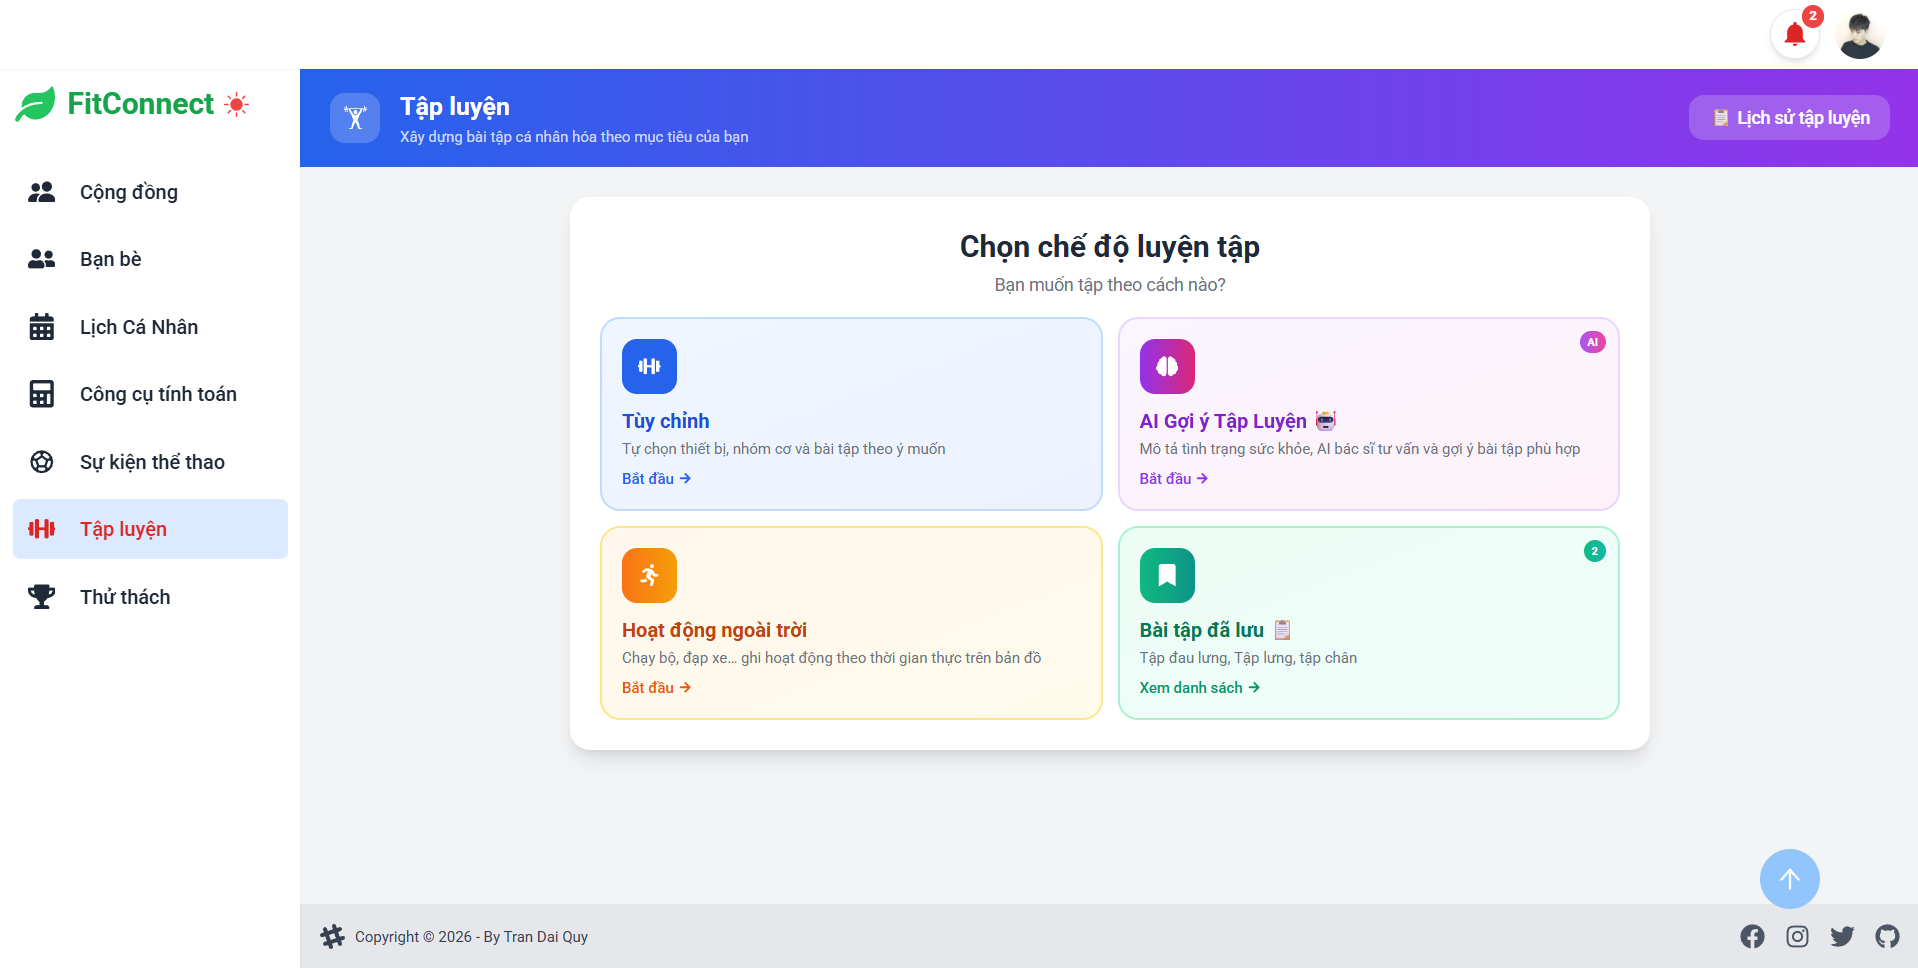
\includegraphics[width=0.85\textwidth]{Images/IMG/Tapluyen/tapluyen.jpg}
    \vspace{1em}
    \caption{(a) Tổng quan tập luyện cá nhân}
    \label{fig:ui_tapluyen_overview}
\end{figure}

\begin{figure}[H]
    \centering
    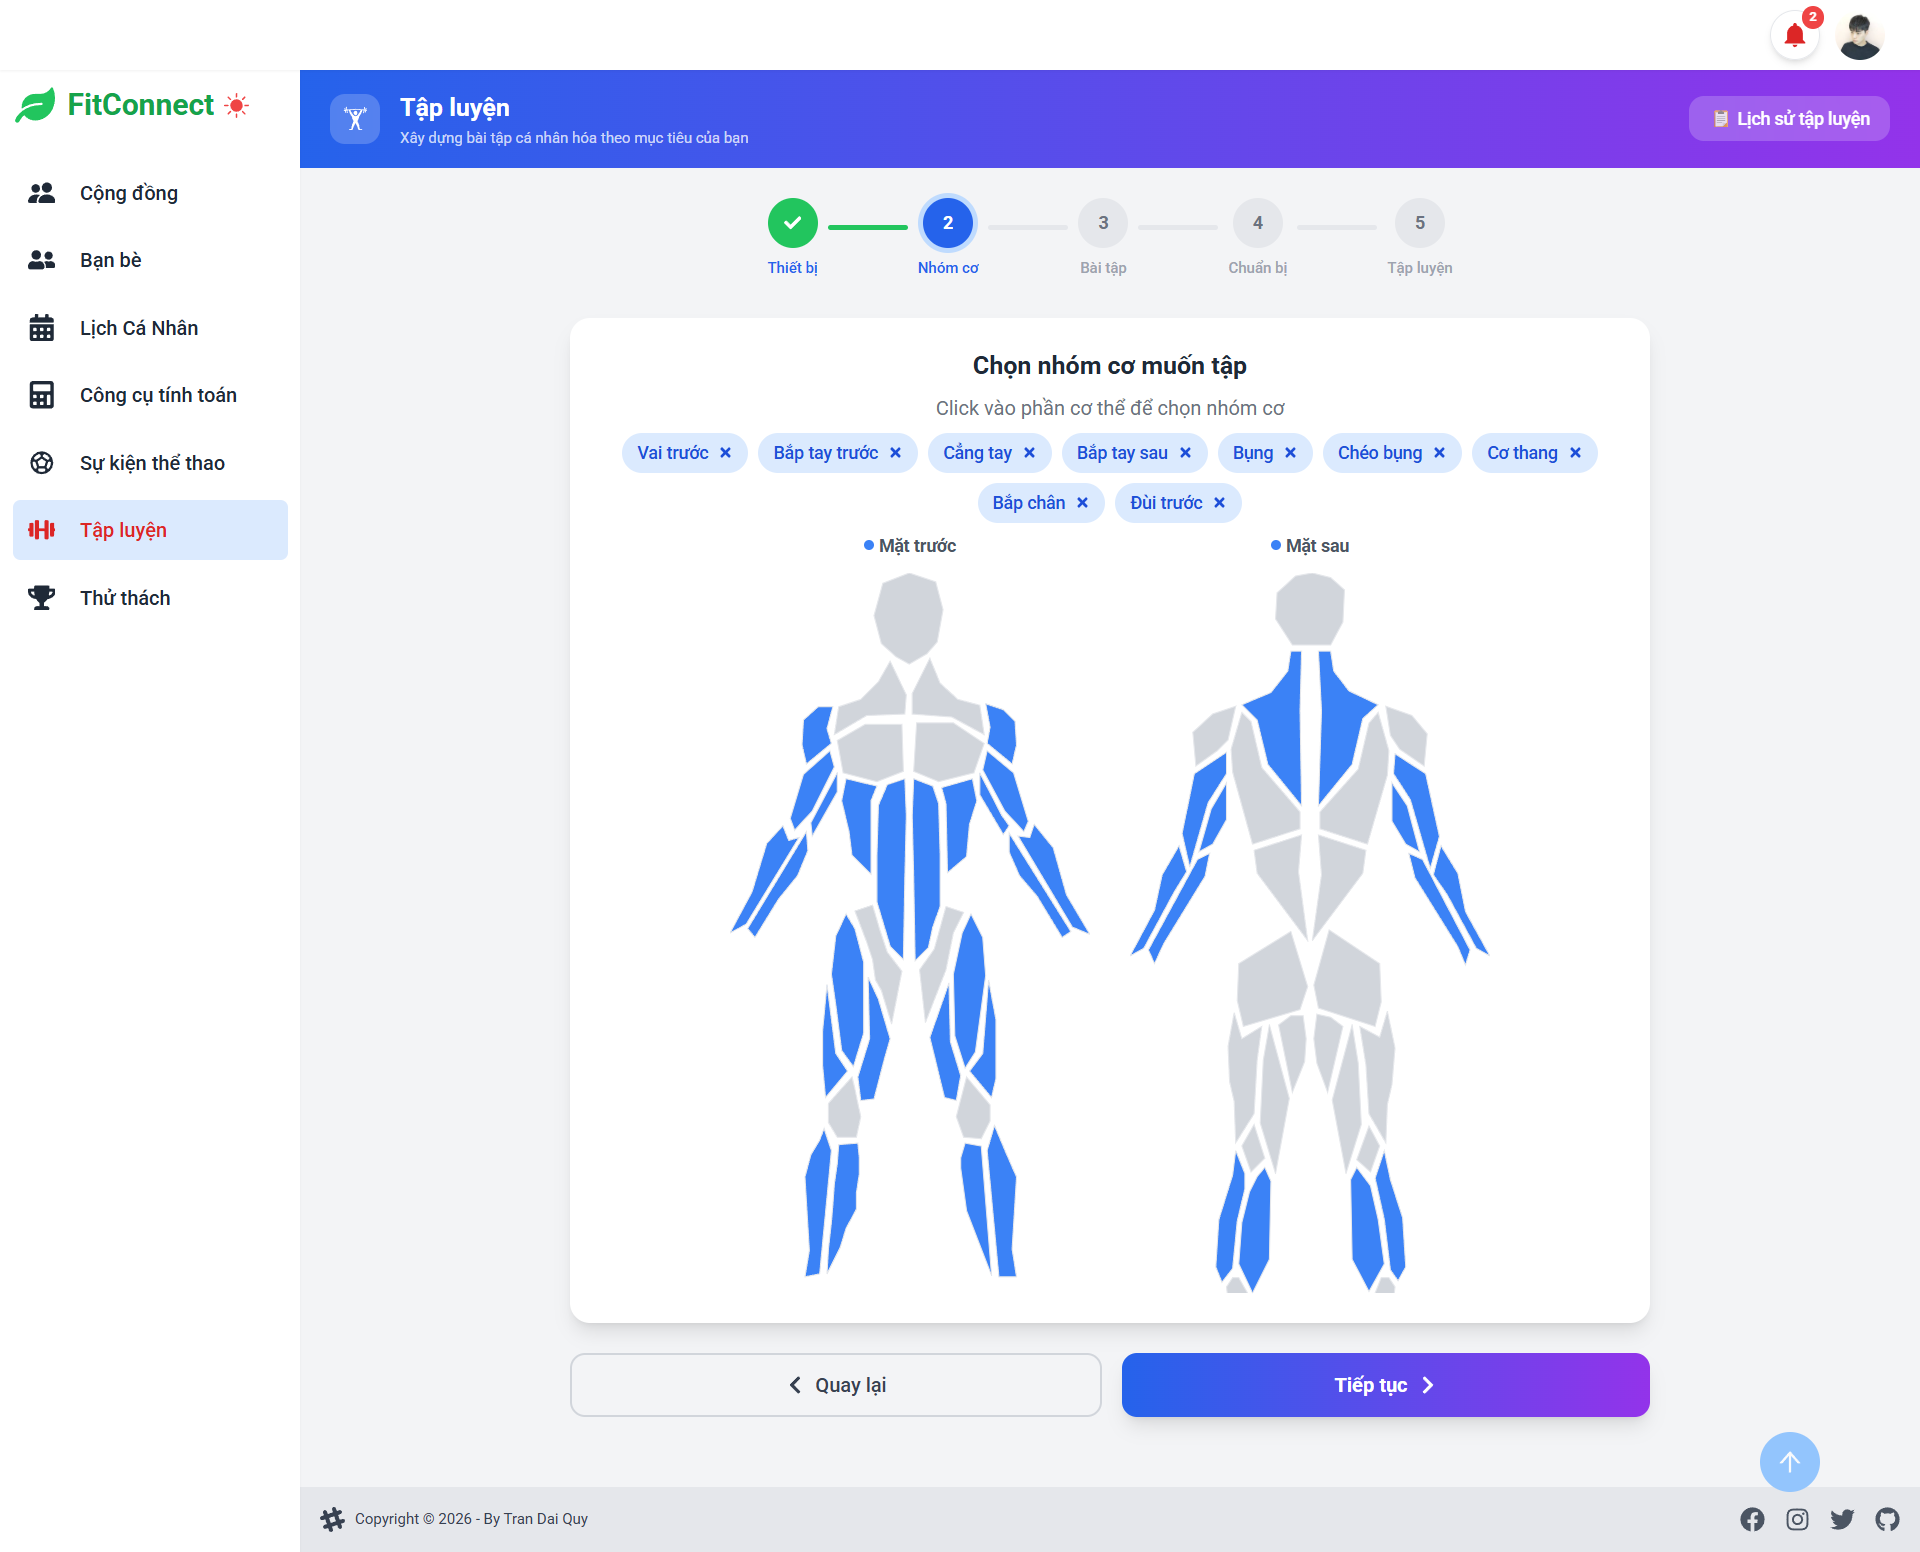
\includegraphics[width=0.85\textwidth]{Images/IMG/Tapluyen/nhomco.jpg}
    \vspace{1em}
    \caption{(b) Lọc bài tập theo nhóm cơ mục tiêu}
    \label{fig:ui_nhomco}
\end{figure}

\begin{figure}[H]
    \centering
    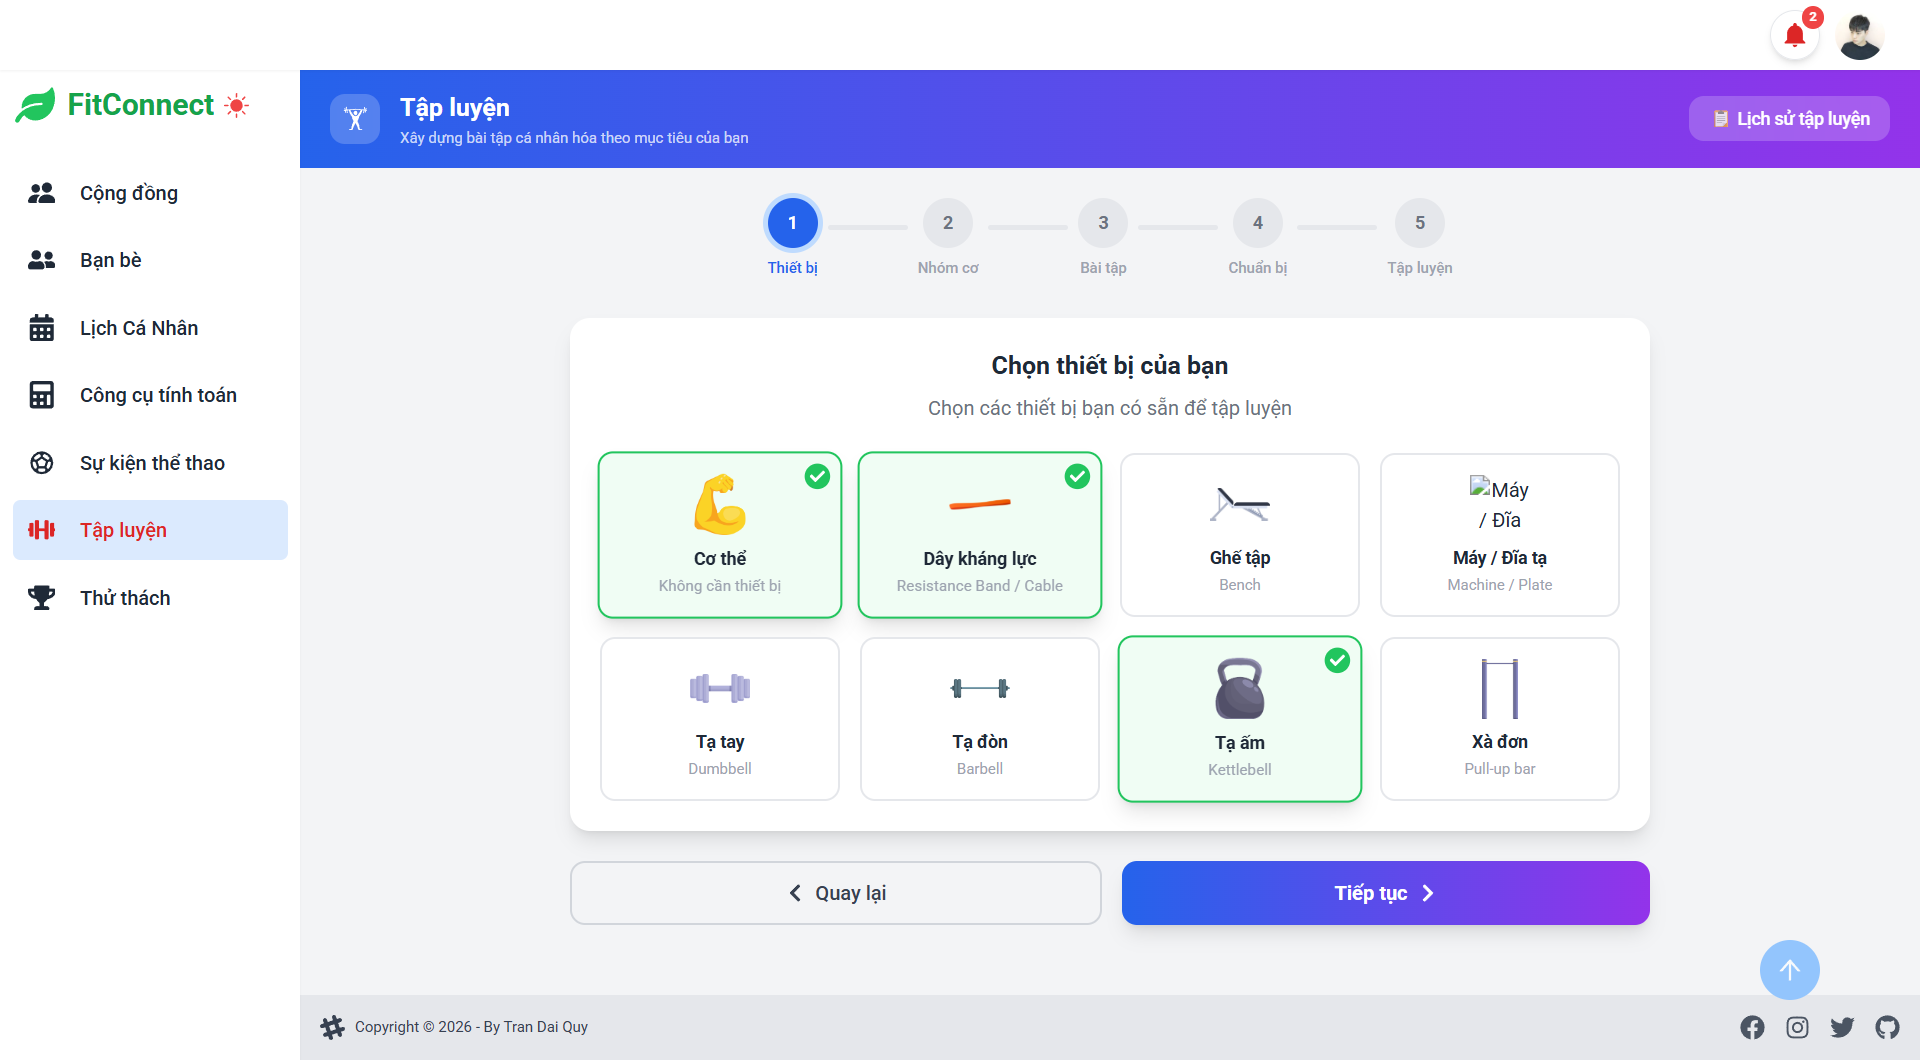
\includegraphics[width=0.85\textwidth]{Images/IMG/Tapluyen/thietbi.jpg}
    \vspace{1em}
    \caption{(c) Lọc bài tập theo thiết bị dụng cụ}
    \label{fig:ui_thietbi}
\end{figure}

\begin{figure}[H]
    \centering
    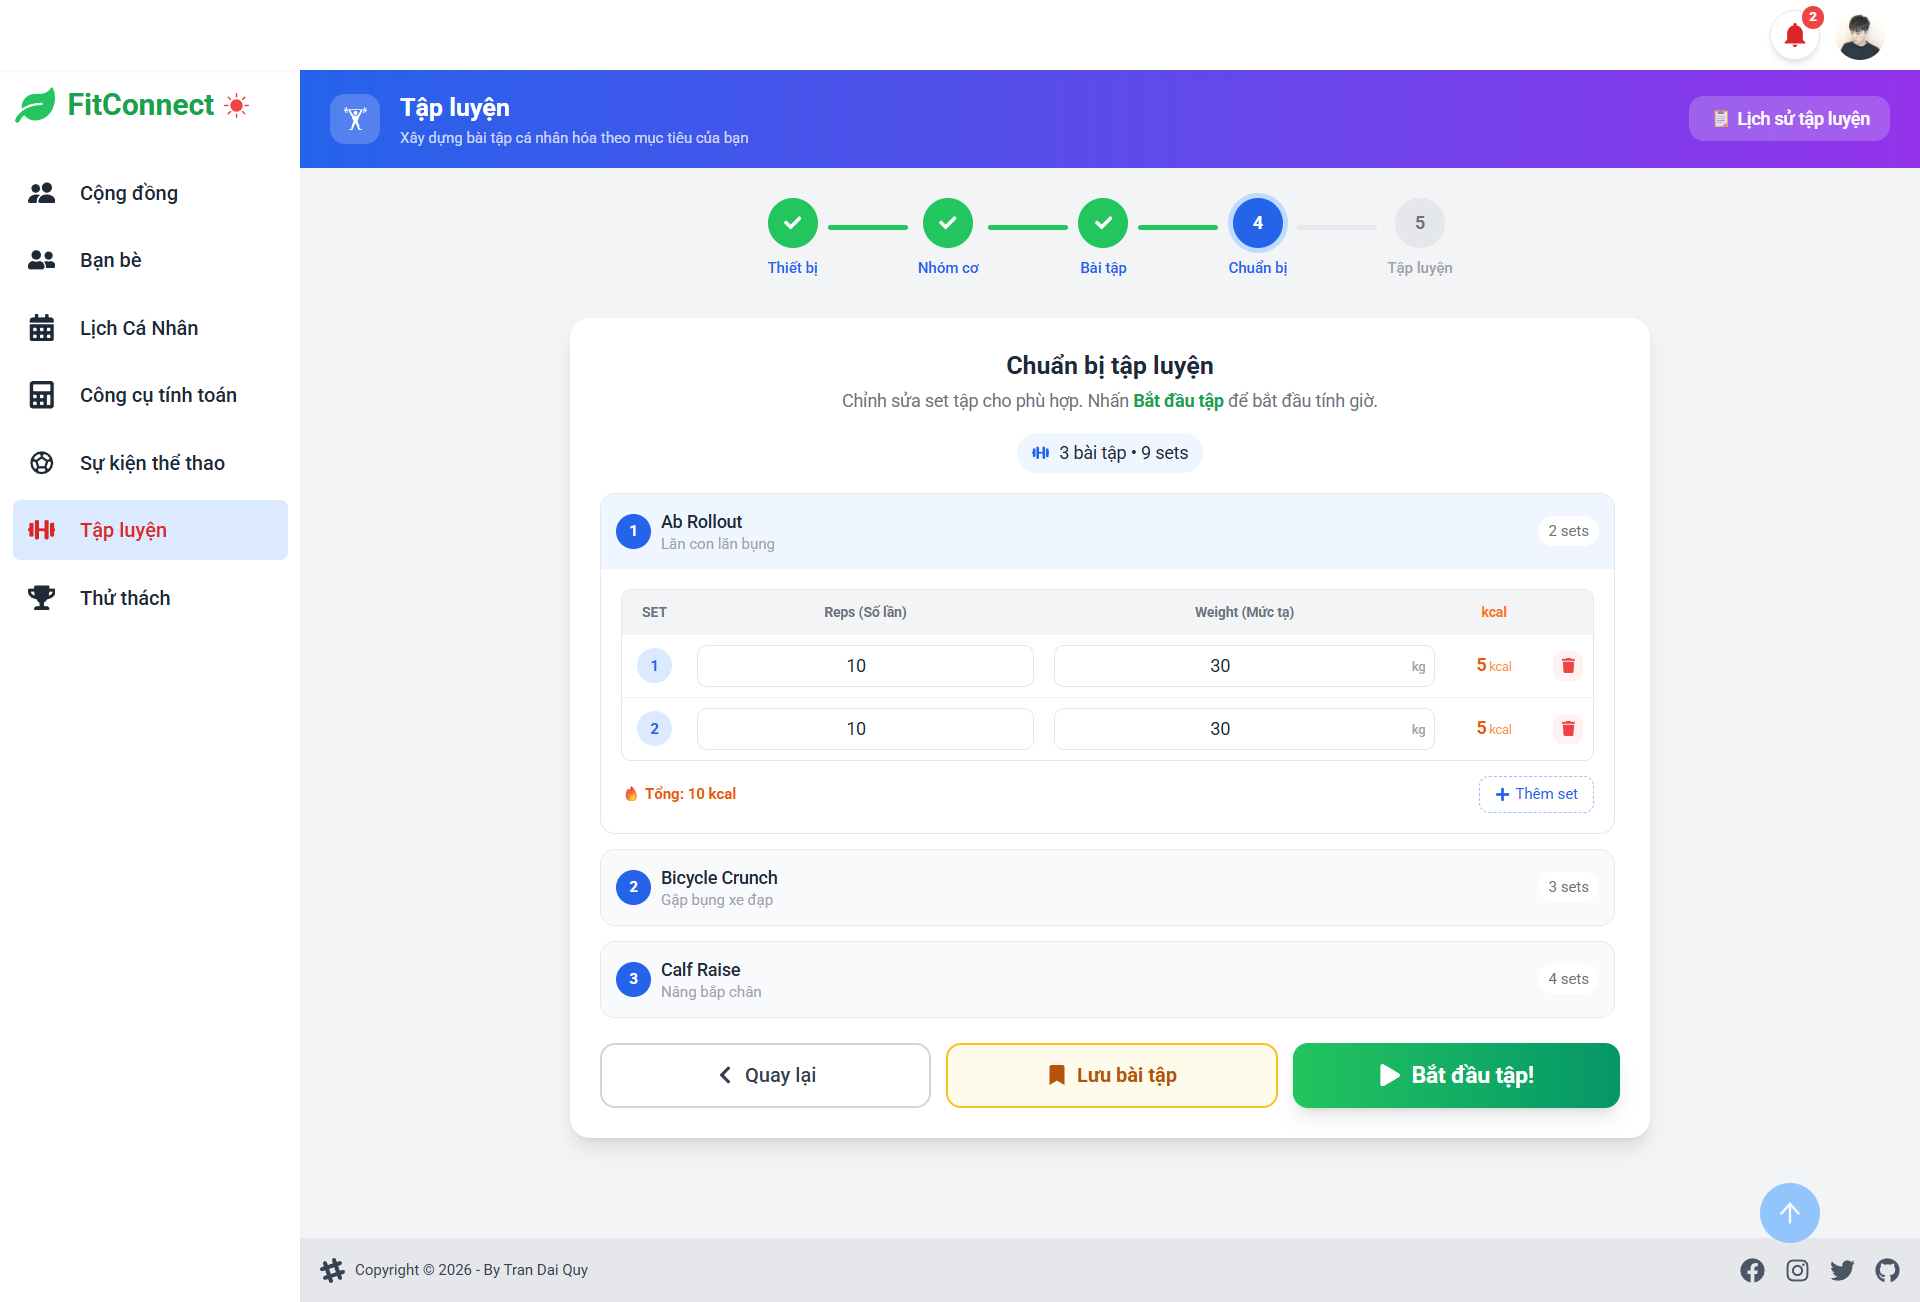
\includegraphics[width=0.85\textwidth]{Images/IMG/Tapluyen/chuanbitapluyen.jpg}
    \vspace{1em}
    \caption{(d) Chuẩn bị buổi tập}
    \label{fig:ui_chuanbitap}
\end{figure}

\begin{figure}[H]
    \centering
    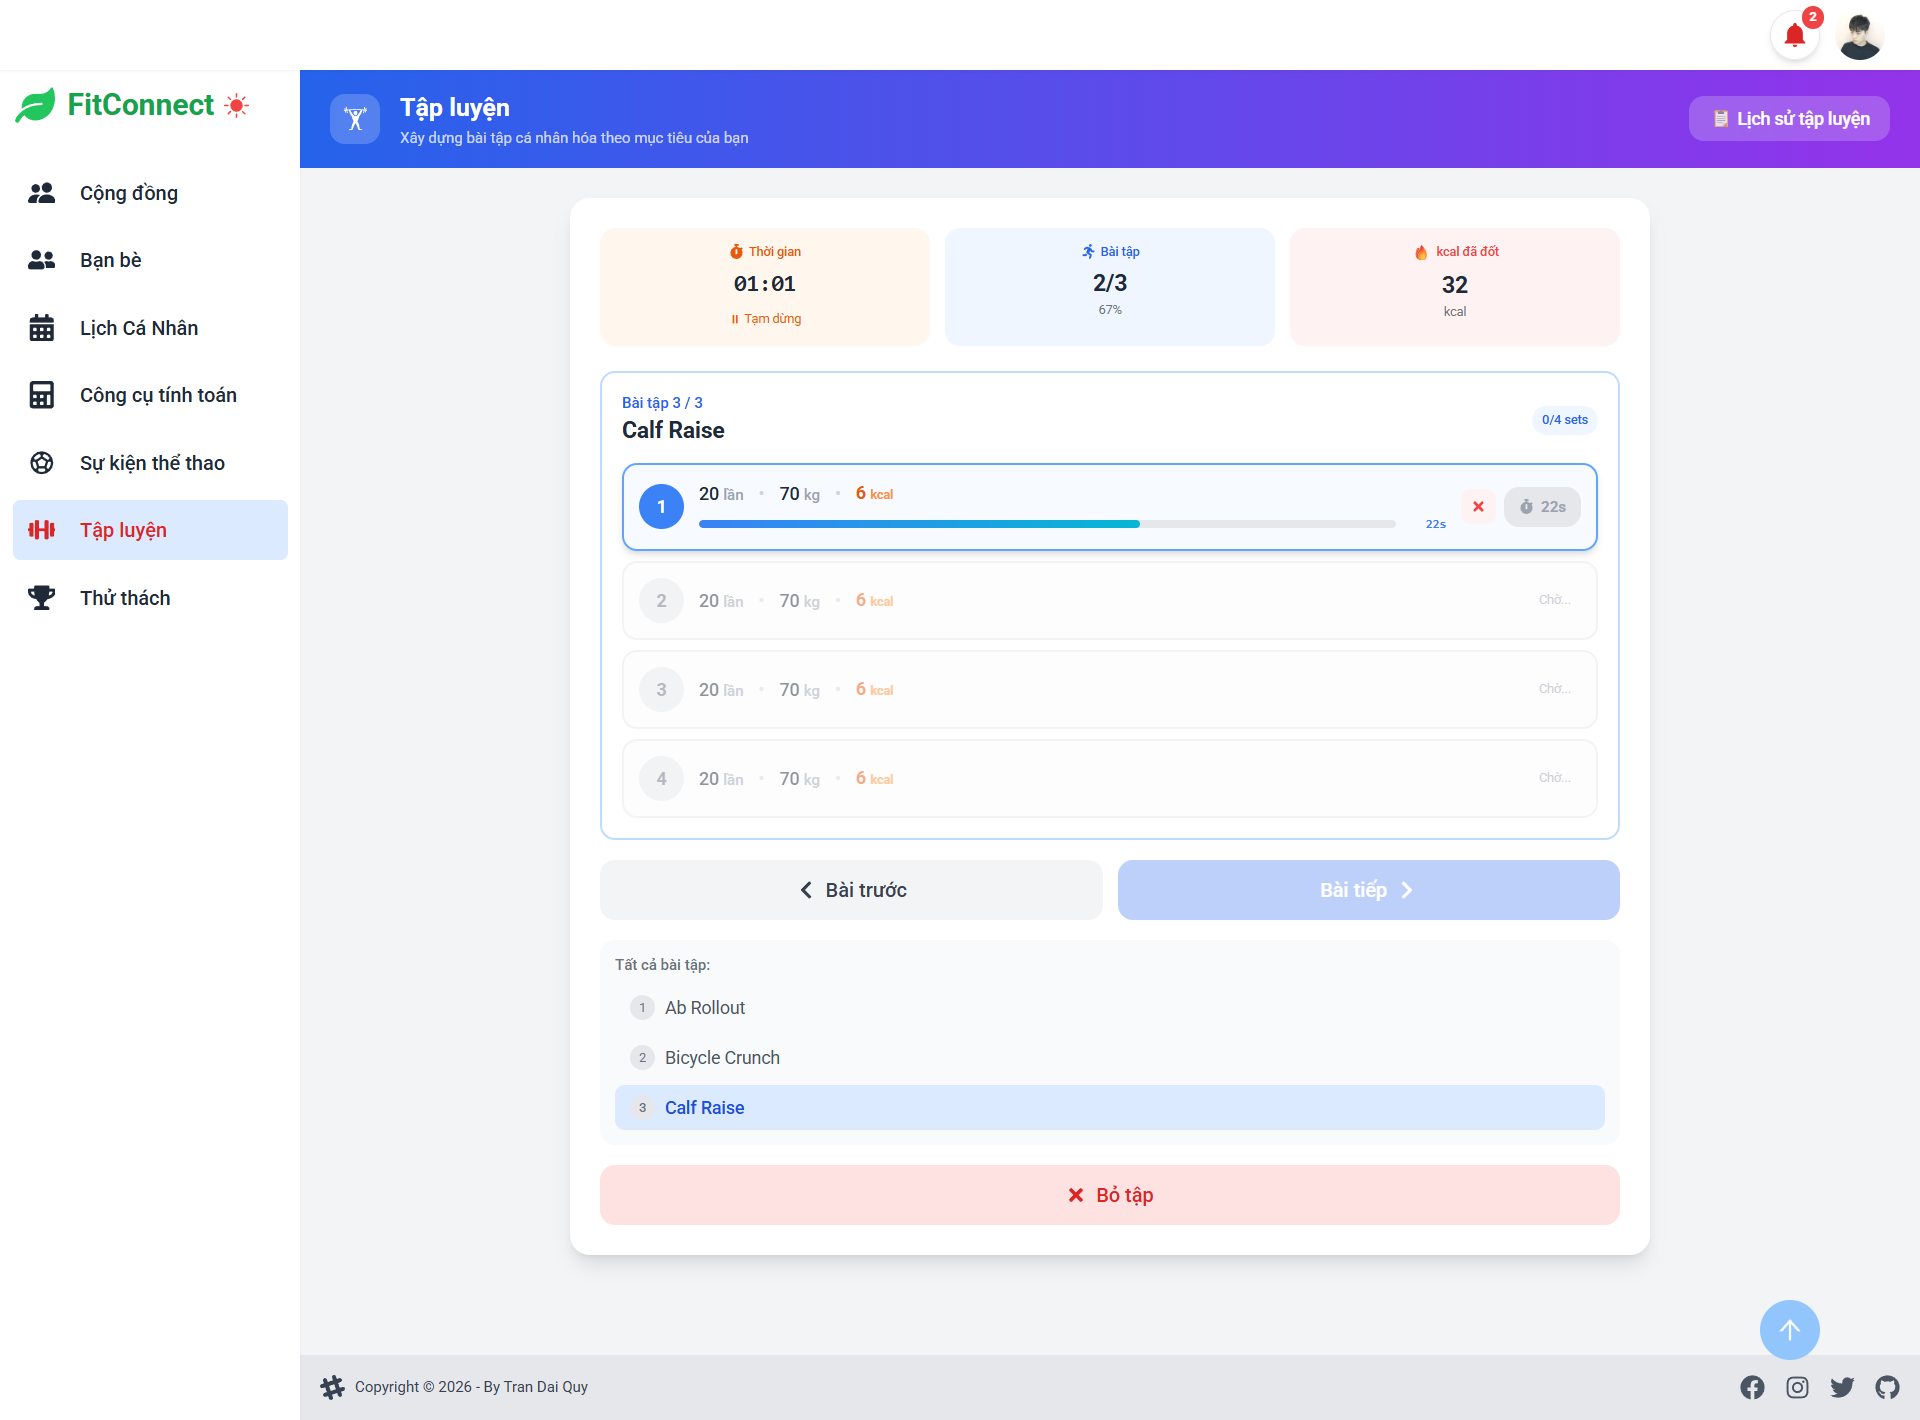
\includegraphics[width=0.85\textwidth]{Images/IMG/Tapluyen/tienhanhtapluyen.jpg}
    \vspace{1em}
    \caption{(e) Tiến hành tập luyện tại chỗ}
    \label{fig:ui_tienhanhtap}
\end{figure}

\begin{figure}[H]
    \centering
    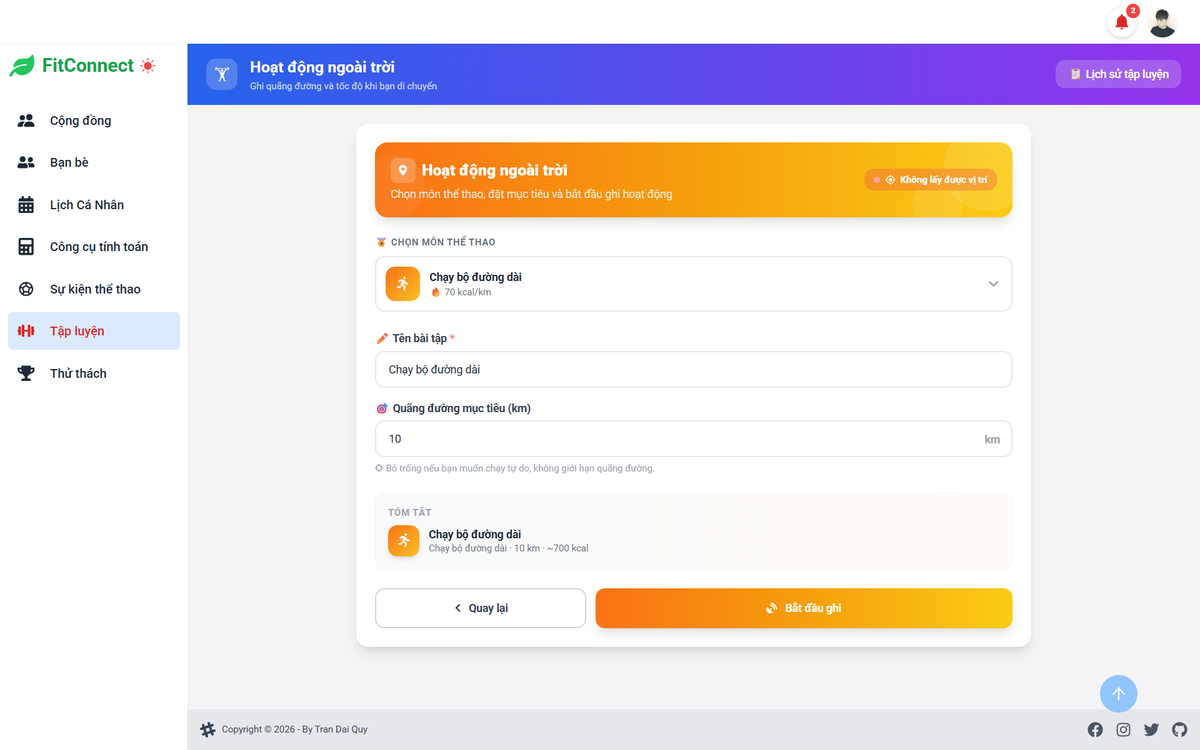
\includegraphics[width=0.85\textwidth]{Images/IMG/Tapluyen/tapluyenchaybo.jpg}
    \vspace{1em}
    \caption{(f) Tập luyện ngoài trời với ghi nhận GPS}
    \label{fig:ui_chaybo}
\end{figure}

% ─── 6. CÔNG CỤ TÍNH TOÁN ────────────────────────────────────────────────────
\paragraph{Nhóm tính năng Công cụ tính toán}
Phân hệ Công cụ tính toán cung cấp bộ đo lường chỉ số sinh lý học cá nhân. Người dùng nhập các thông số cơ thể để hệ thống tính toán và trả về kết quả BMI, BMR, TDEE cùng phân tích chi tiết. Trợ lý AI tích hợp phân tích tình trạng thể trạng và đề xuất lộ trình cải thiện phù hợp. Màn hình lịch sử chỉ số hiển thị biểu đồ xu hướng thể trạng theo thời gian, giúp người dùng đánh giá tiến bộ qua từng tuần, từng tháng.

\begin{figure}[H]
    \centering
    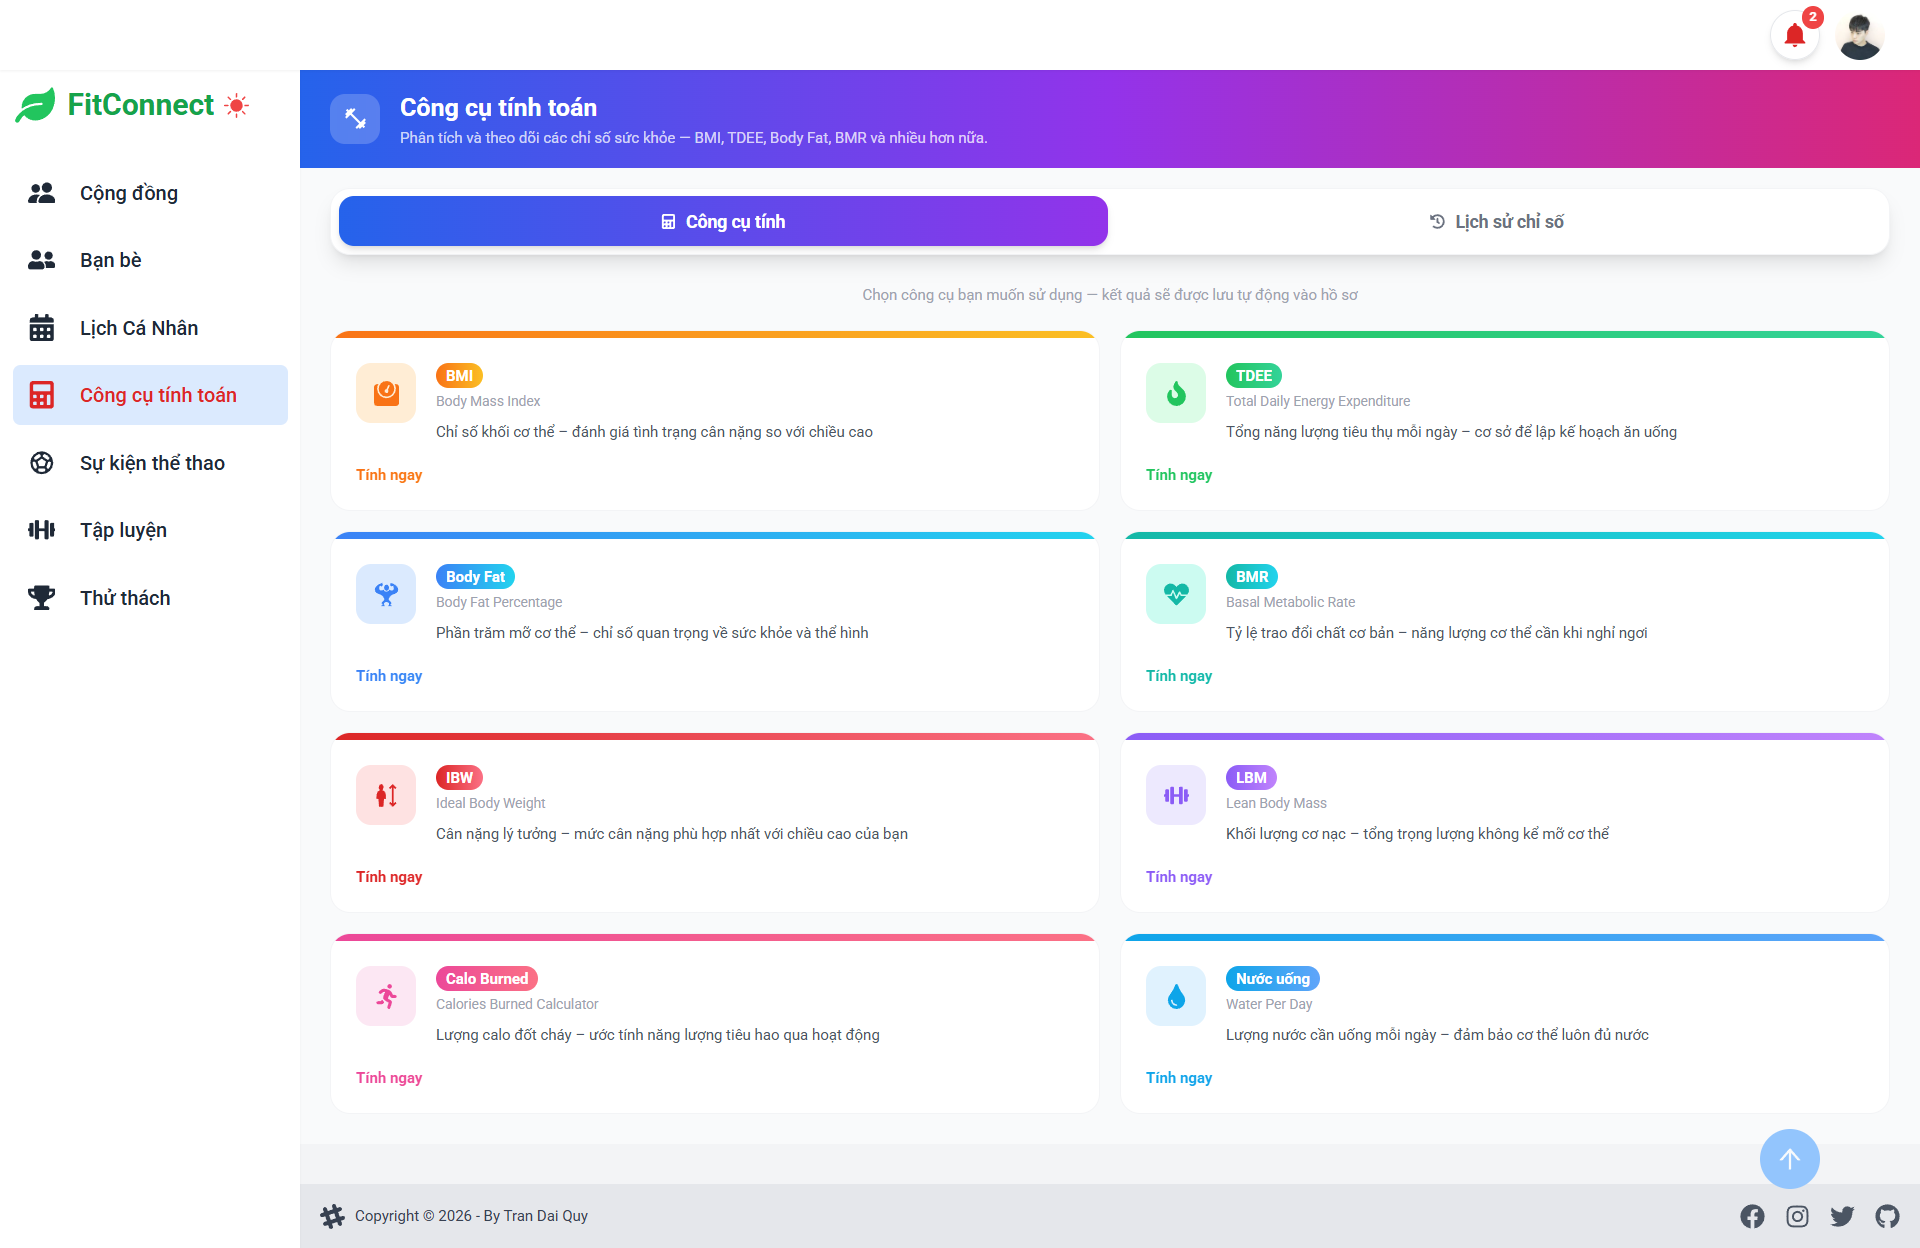
\includegraphics[width=0.85\textwidth]{Images/IMG/Congcusuckhoe/congcutinhtoan.jpg}
    \vspace{1em}
    \caption{(a) Công cụ tính toán chỉ số sức khỏe}
    \label{fig:ui_congcutinhtoan}
\end{figure}

\begin{figure}[H]
    \centering
    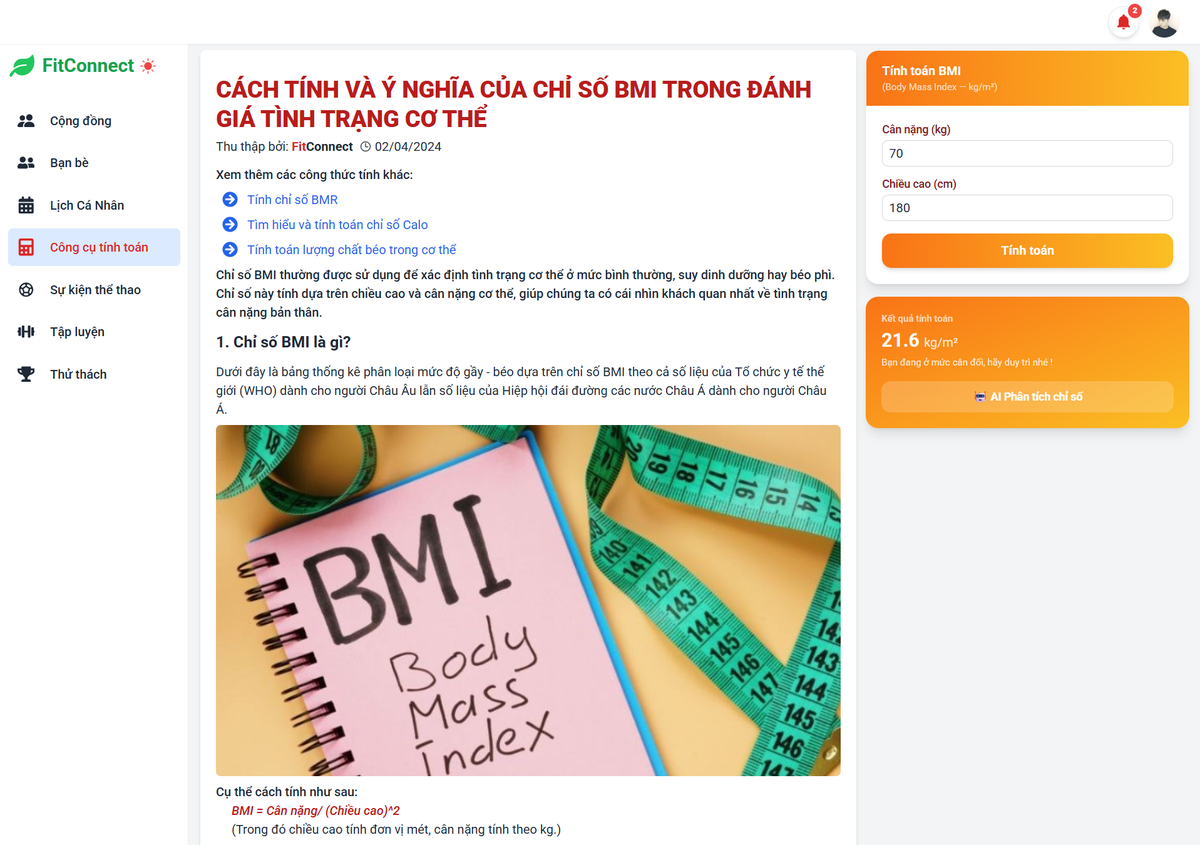
\includegraphics[width=0.85\textwidth]{Images/IMG/Congcusuckhoe/chitiettinhtoan.jpg}
    \vspace{1em}
    \caption{(b) Kết quả chi tiết BMI, BMR, TDEE}
    \label{fig:ui_chitiettinhtoan}
\end{figure}

\begin{figure}[H]
    \centering
    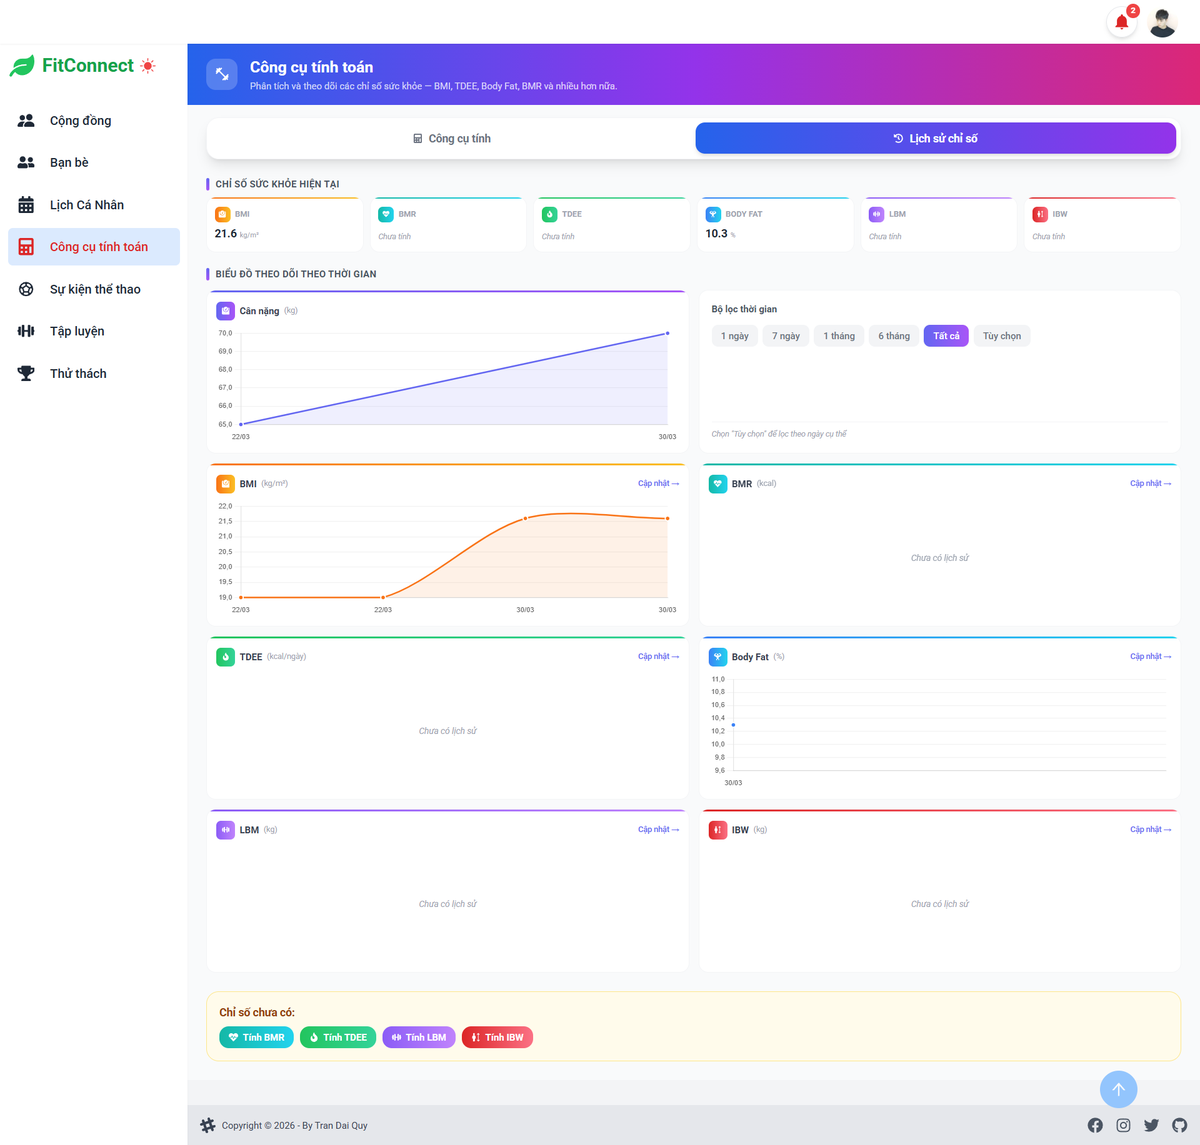
\includegraphics[width=0.85\textwidth]{Images/IMG/Congcusuckhoe/lichsuchiso.jpg}
    \vspace{1em}
    \caption{(c) Lịch sử chỉ số sức khỏe theo thời gian}
    \label{fig:ui_lichsuchiso}
\end{figure}

% ─── 7. BẠN BÈ ────────────────────────────────────────────────────────────────
\paragraph{Nhóm tính năng Bạn bè}
Phân hệ Bạn bè cho phép người dùng xây dựng và quản lý mạng lưới quan hệ xã hội trong nền tảng. Người dùng có thể tìm kiếm thành viên theo tên và tiêu chí sở thích, thực hiện kết bạn hoặc theo dõi (Follow). Giao diện danh sách bạn bè hiển thị trạng thái hoạt động và tóm tắt thành tích nổi bật của từng người trong mạng lưới kết nối.

\begin{figure}[H]
    \centering
    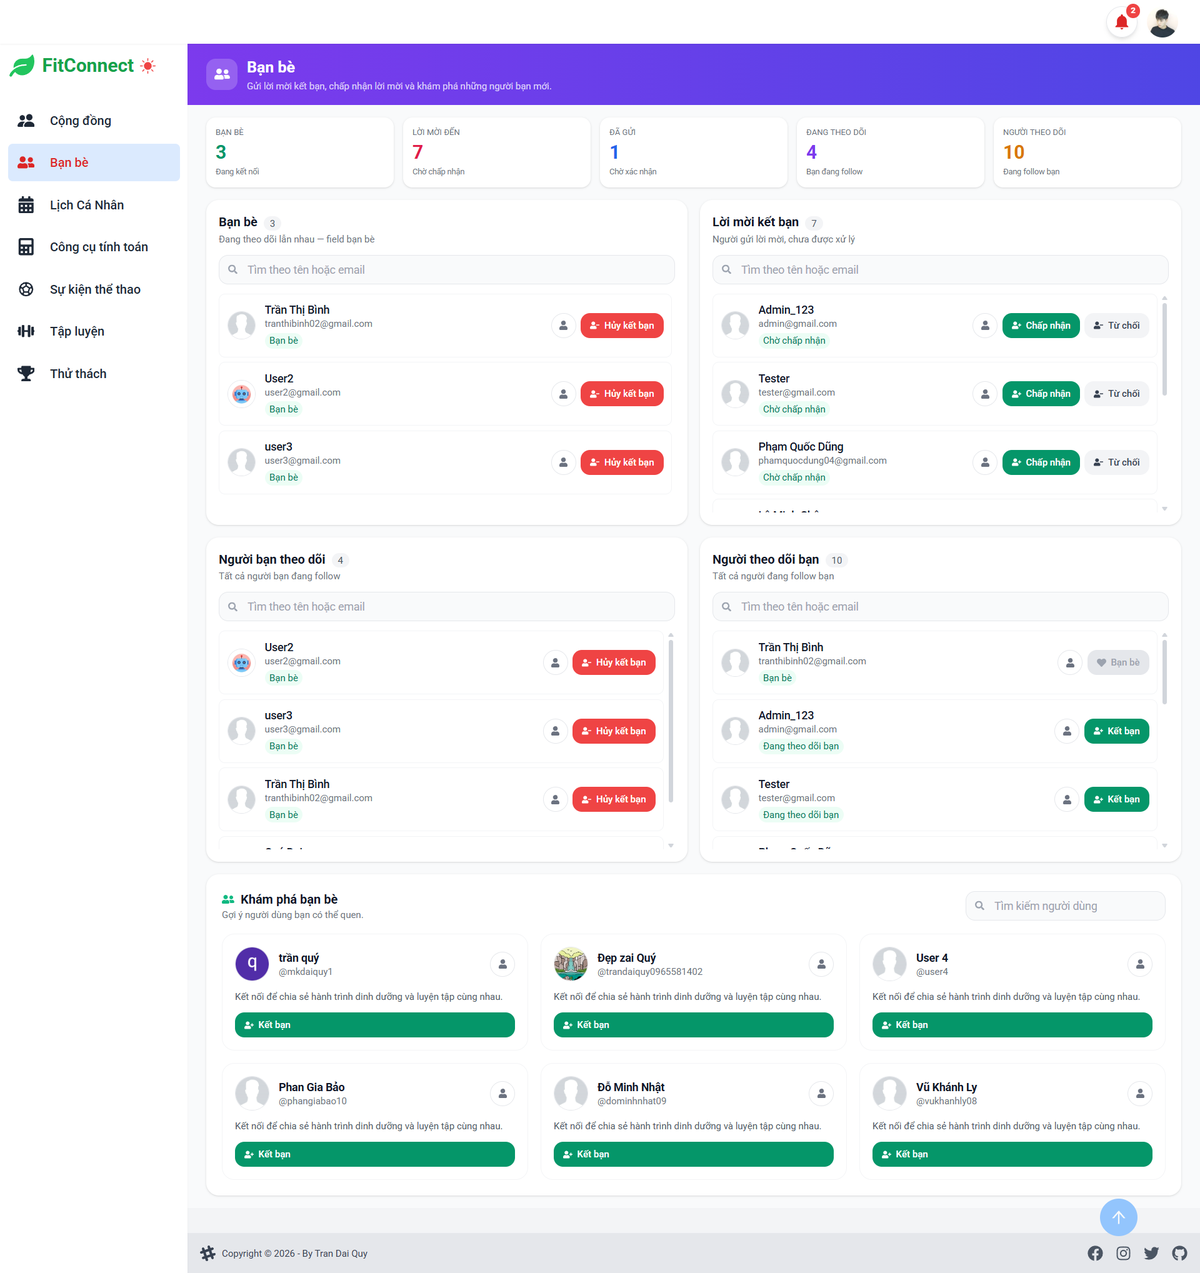
\includegraphics[width=0.85\textwidth]{Images/IMG/Banbe/banbe.jpg}
    \vspace{1em}
    \caption{Màn hình nhóm tính năng Bạn bè - Danh sách kết nối và theo dõi mạng lưới}
    \label{fig:ui_banbe}
\end{figure}

% ─── 8. LỊCH CÁ NHÂN VÀ THÔNG BÁO ───────────────────────────────────────────
\paragraph{Nhóm tính năng Lịch cá nhân và Thông báo}
Giao diện Lịch cá nhân (Calendar) là trung tâm điều phối thời gian của người dùng, tổng hợp tự động toàn bộ các mốc thời gian từ sự kiện thể thao, thử thách và lịch tập luyện đã đặt. Người dùng có thể xem tổng quan theo tuần/tháng và nhận thông báo nhắc nhở theo thời gian thực khi đến hạn thực hiện mục tiêu hoặc khi bạn bè tương tác.

\begin{figure}[H]
    \centering
    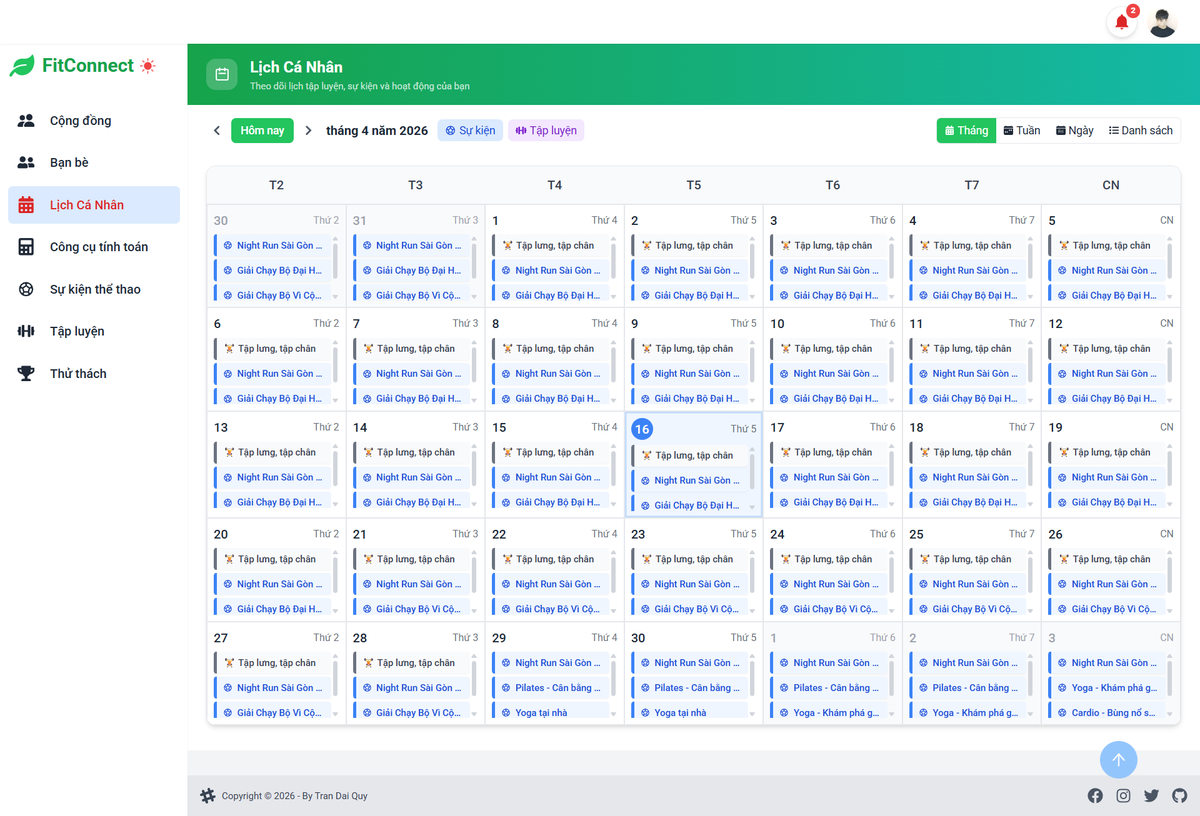
\includegraphics[width=0.85\textwidth]{Images/IMG/lichcanhan/lichcanhan.jpg}
    \vspace{1em}
    \caption{Màn hình nhóm tính năng Lịch cá nhân - Tổng hợp lịch trình sự kiện, thử thách và tập luyện}
    \label{fig:ui_lichcanhan}
\end{figure}

% ─── 9. QUẢN LÝ HỆ THỐNG ADMIN ───────────────────────────────────────────────
\paragraph{Nhóm tính năng Quản lý hệ thống của Admin}
Phân hệ Quản trị cung cấp bộ công cụ kiểm soát tập trung dành riêng cho Quản trị viên. Dashboard tổng hợp các chỉ số tăng trưởng nền tảng qua biểu đồ trực quan. Quản trị viên có thể xem xét và xử lý báo cáo vi phạm (bài viết, sự kiện), quản lý toàn bộ danh sách người dùng và sự kiện thể thao, đồng thời cấu hình danh mục thể thao dùng làm tiêu chuẩn phân loại trên toàn hệ thống.

\begin{figure}[H]
    \centering
    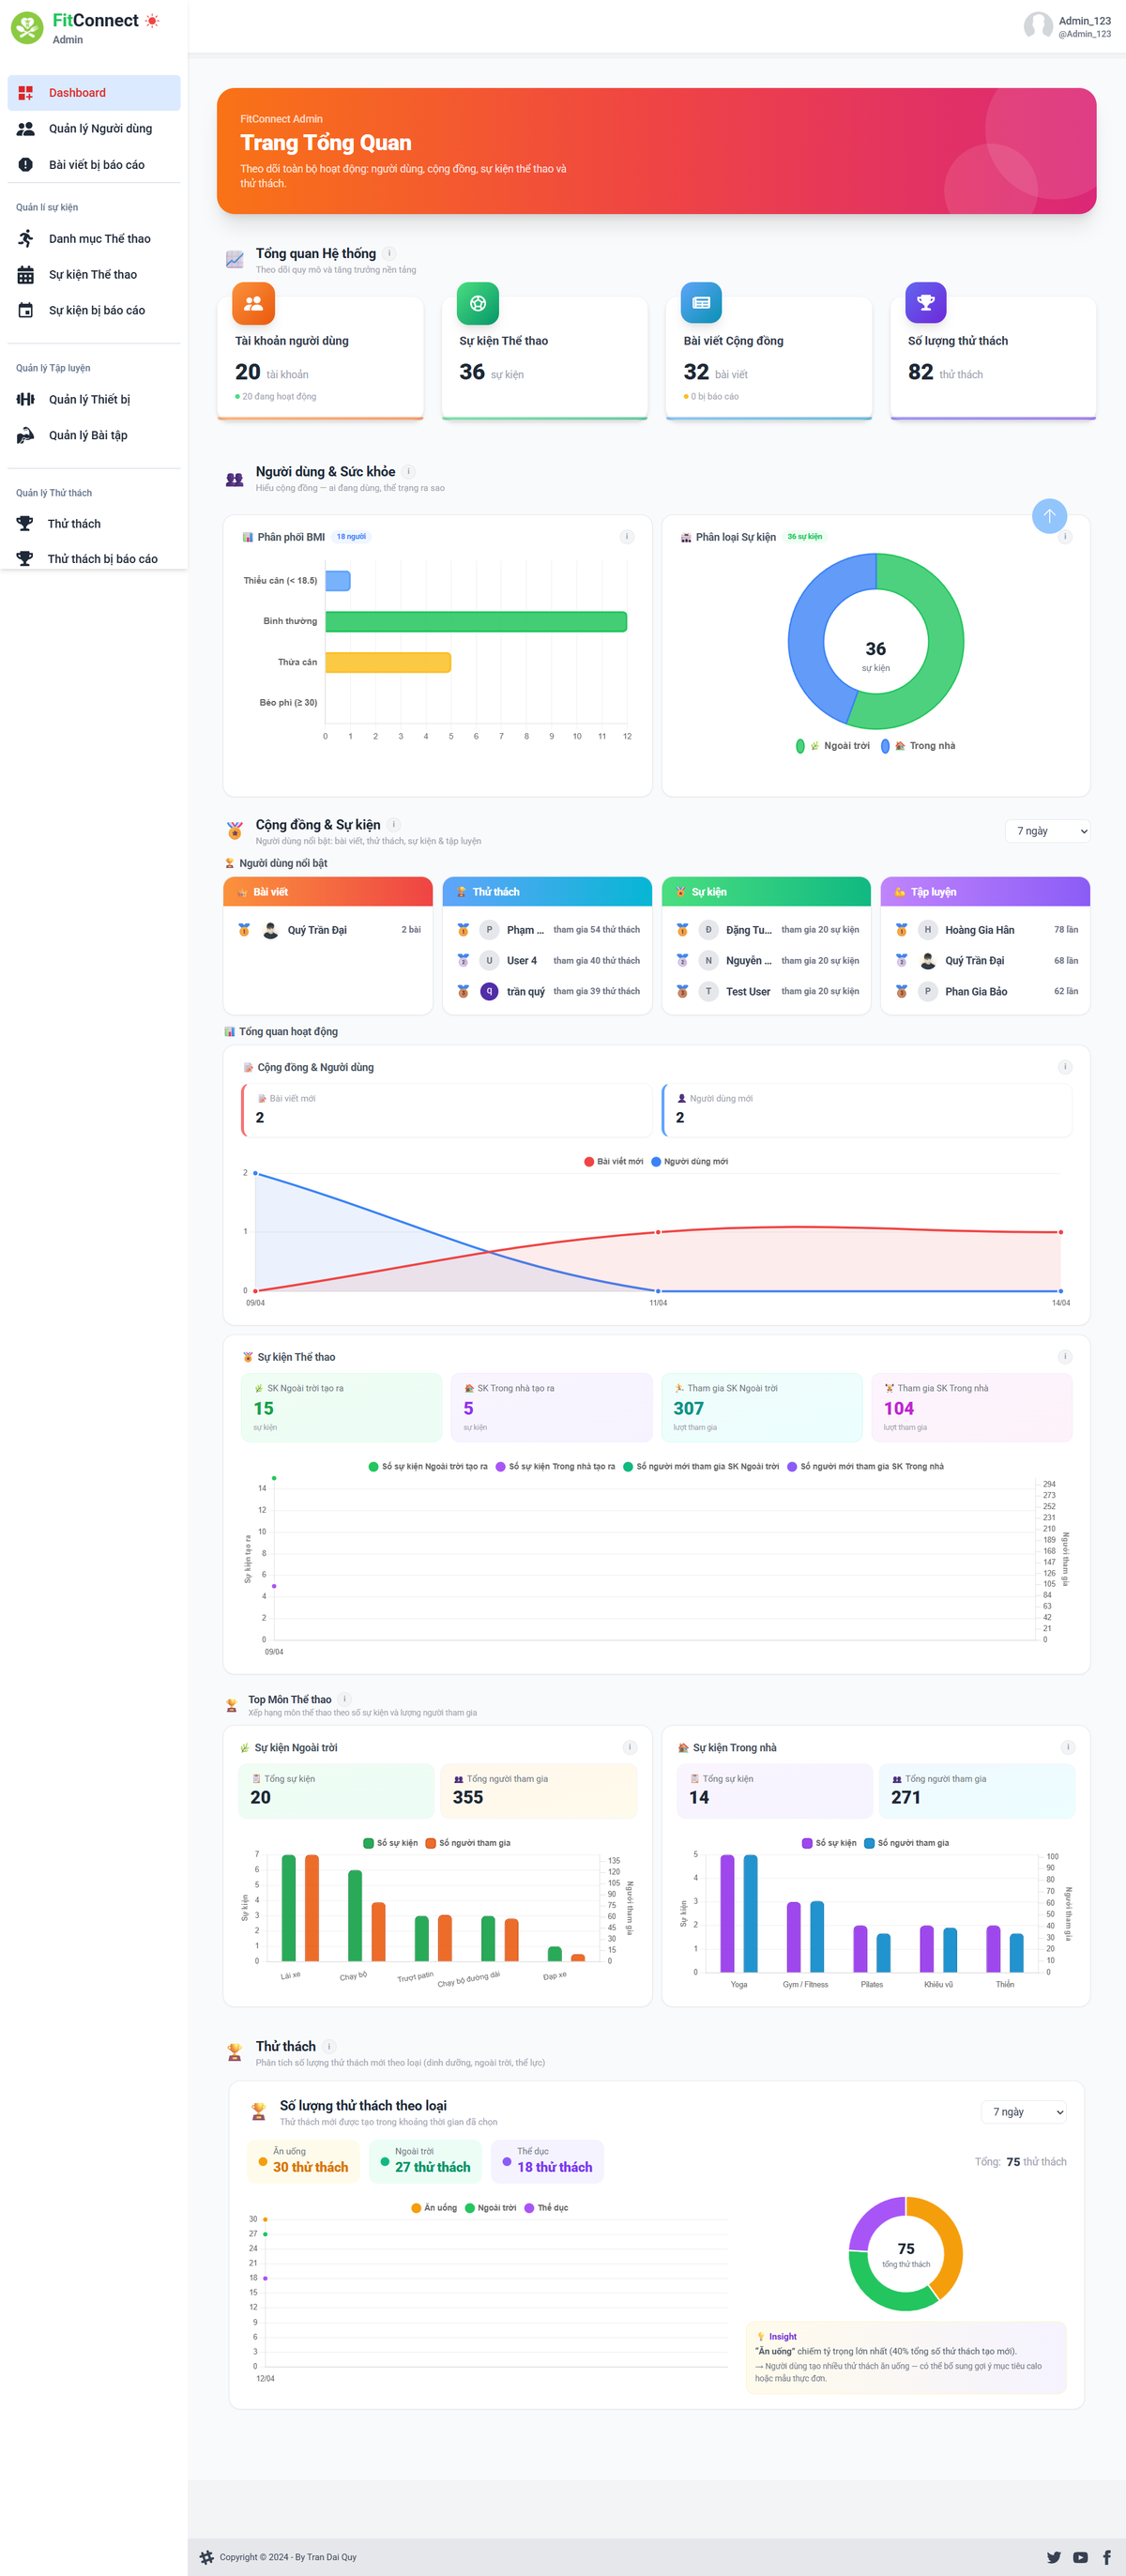
\includegraphics[width=0.85\textwidth]{Images/IMG/TrangAmin/dashboard.jpg}
    \vspace{1em}
    \caption{(a) Dashboard tổng quan hệ thống}
    \label{fig:ui_dashboard}
\end{figure}

\begin{figure}[H]
    \centering
    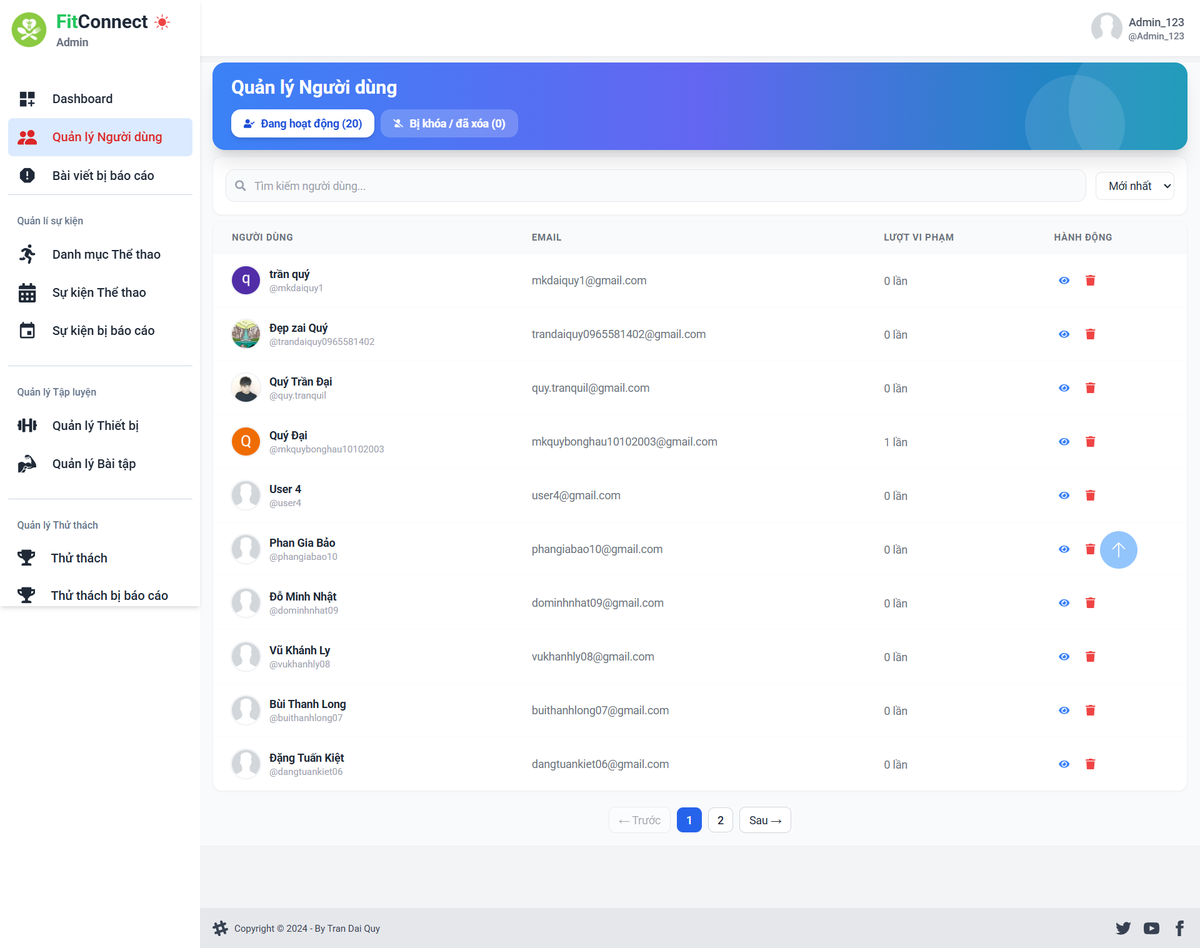
\includegraphics[width=0.85\textwidth]{Images/IMG/TrangAmin/quanlynguoidung.jpg}
    \vspace{1em}
    \caption{(b) Quản lý người dùng}
    \label{fig:ui_admin_user}
\end{figure}

\begin{figure}[H]
    \centering
    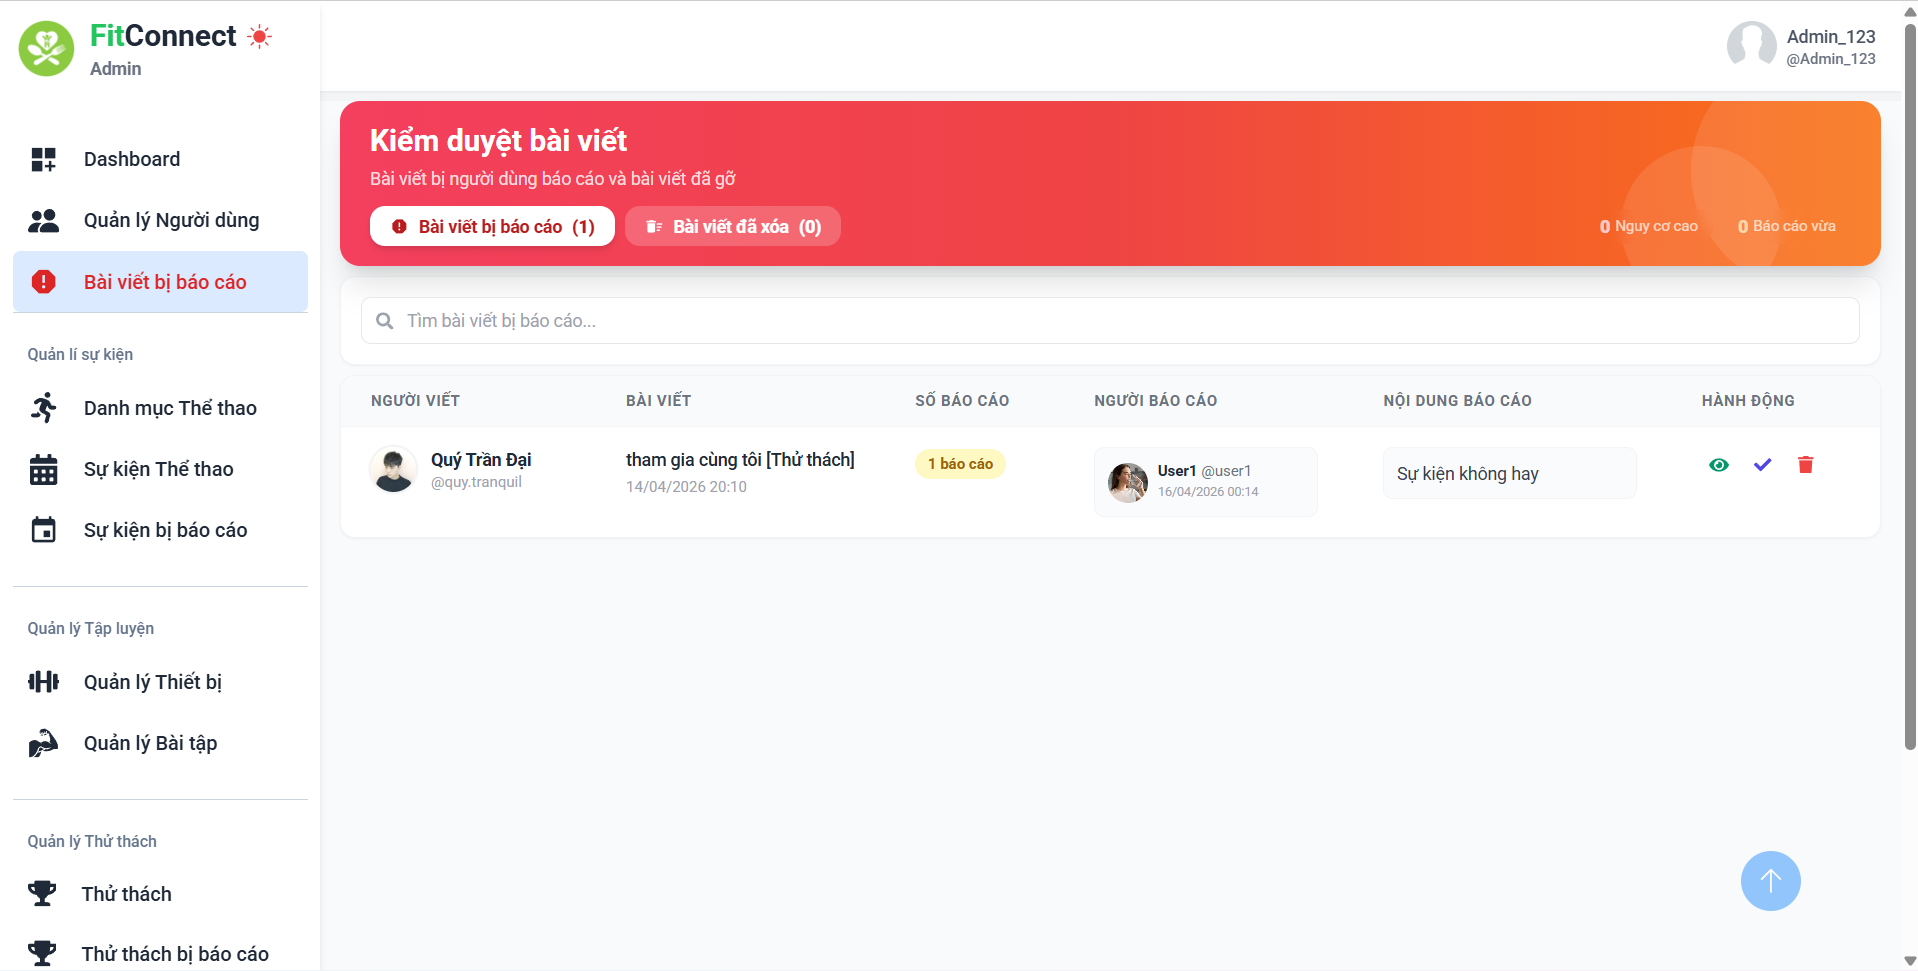
\includegraphics[width=0.85\textwidth]{Images/IMG/TrangAmin/kiemduyetbaiviet.jpg}
    \vspace{1em}
    \caption{(c) Kiểm duyệt bài viết vi phạm}
    \label{fig:ui_kiemduyetbv}
\end{figure}

\begin{figure}[H]
    \centering
    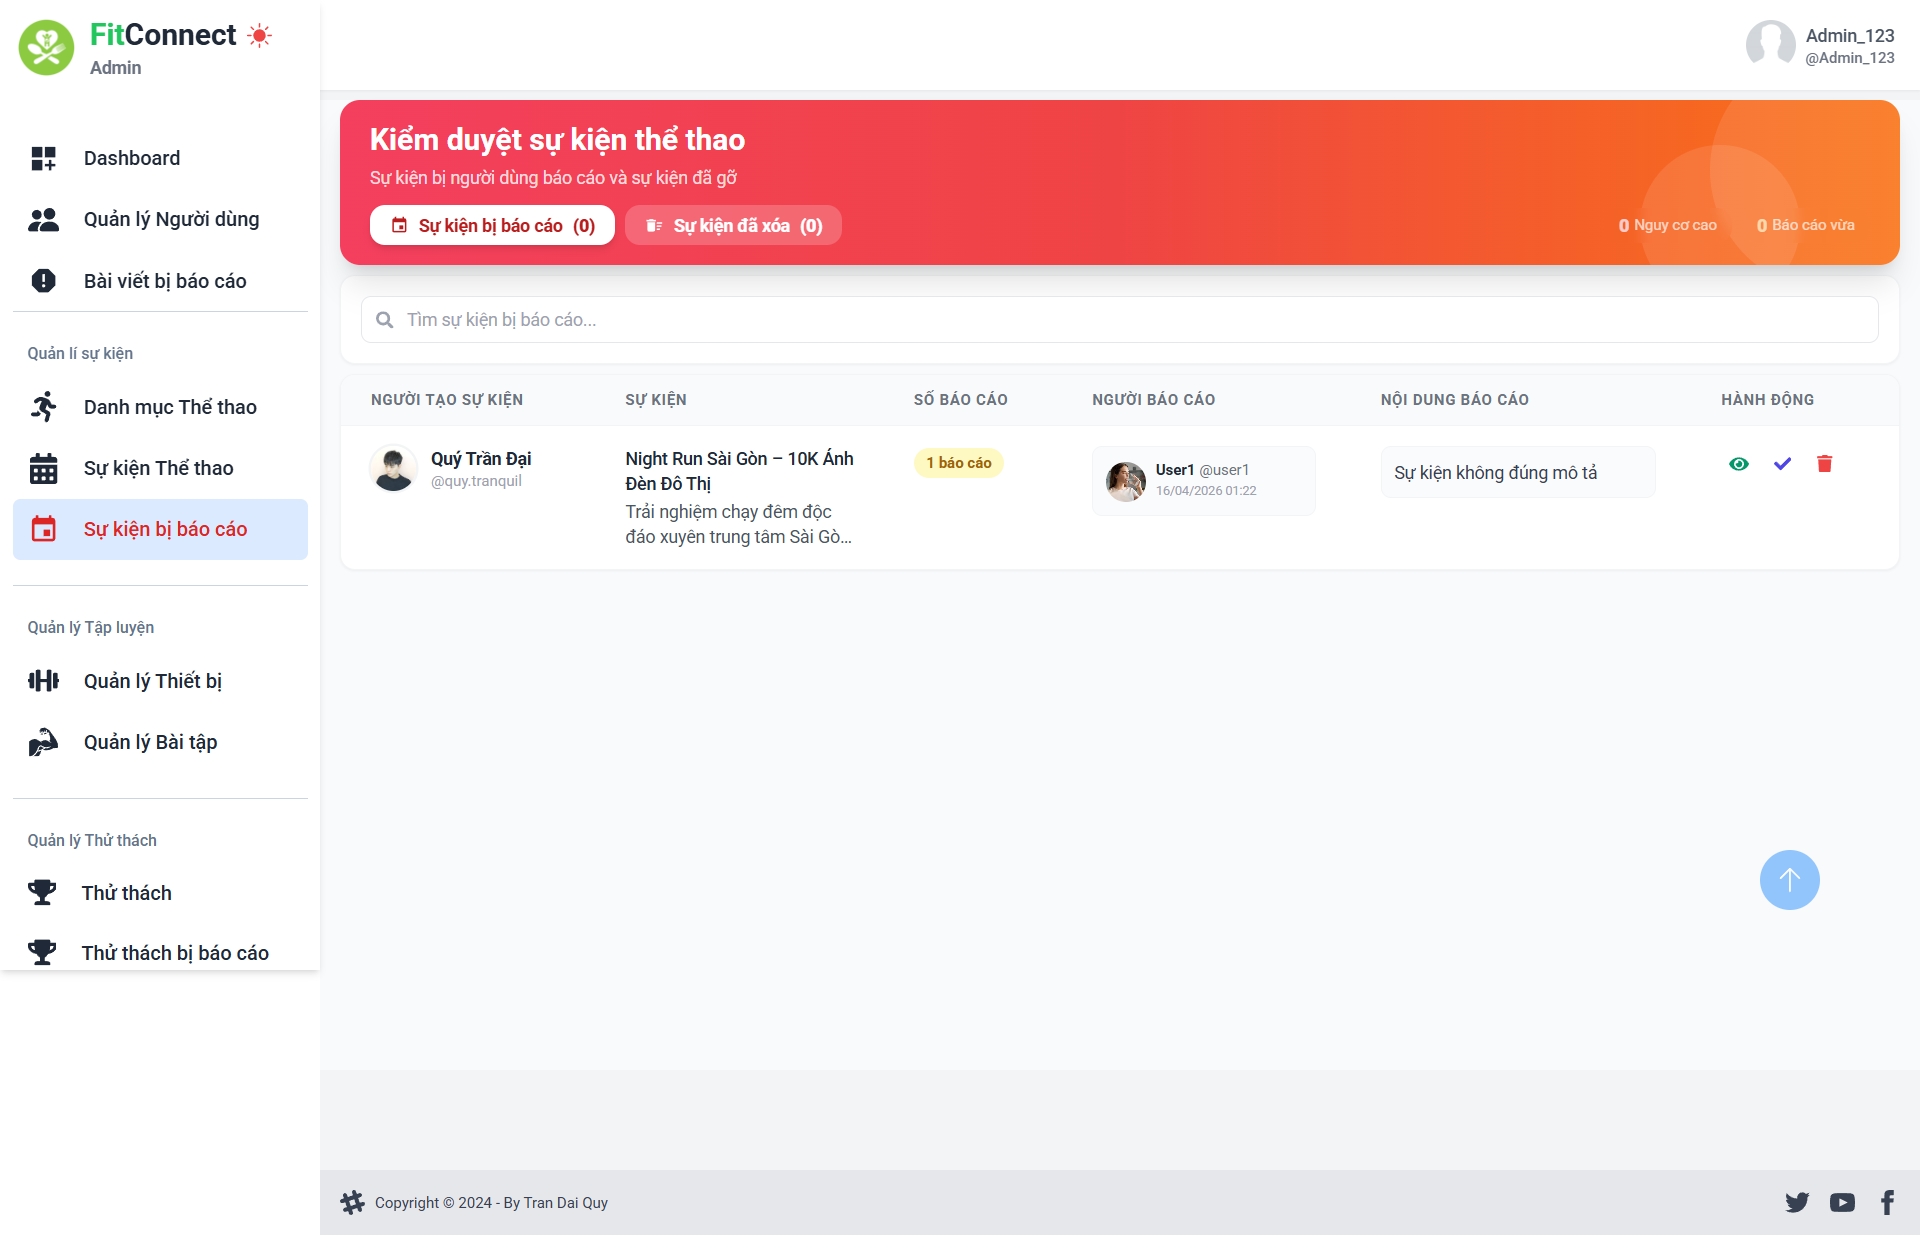
\includegraphics[width=0.85\textwidth]{Images/IMG/TrangAmin/kiemduyetsukien.jpg}
    \vspace{1em}
    \caption{(d) Kiểm duyệt sự kiện thể thao}
    \label{fig:ui_kiemduyetsk}
\end{figure}

\begin{figure}[H]
    \centering
    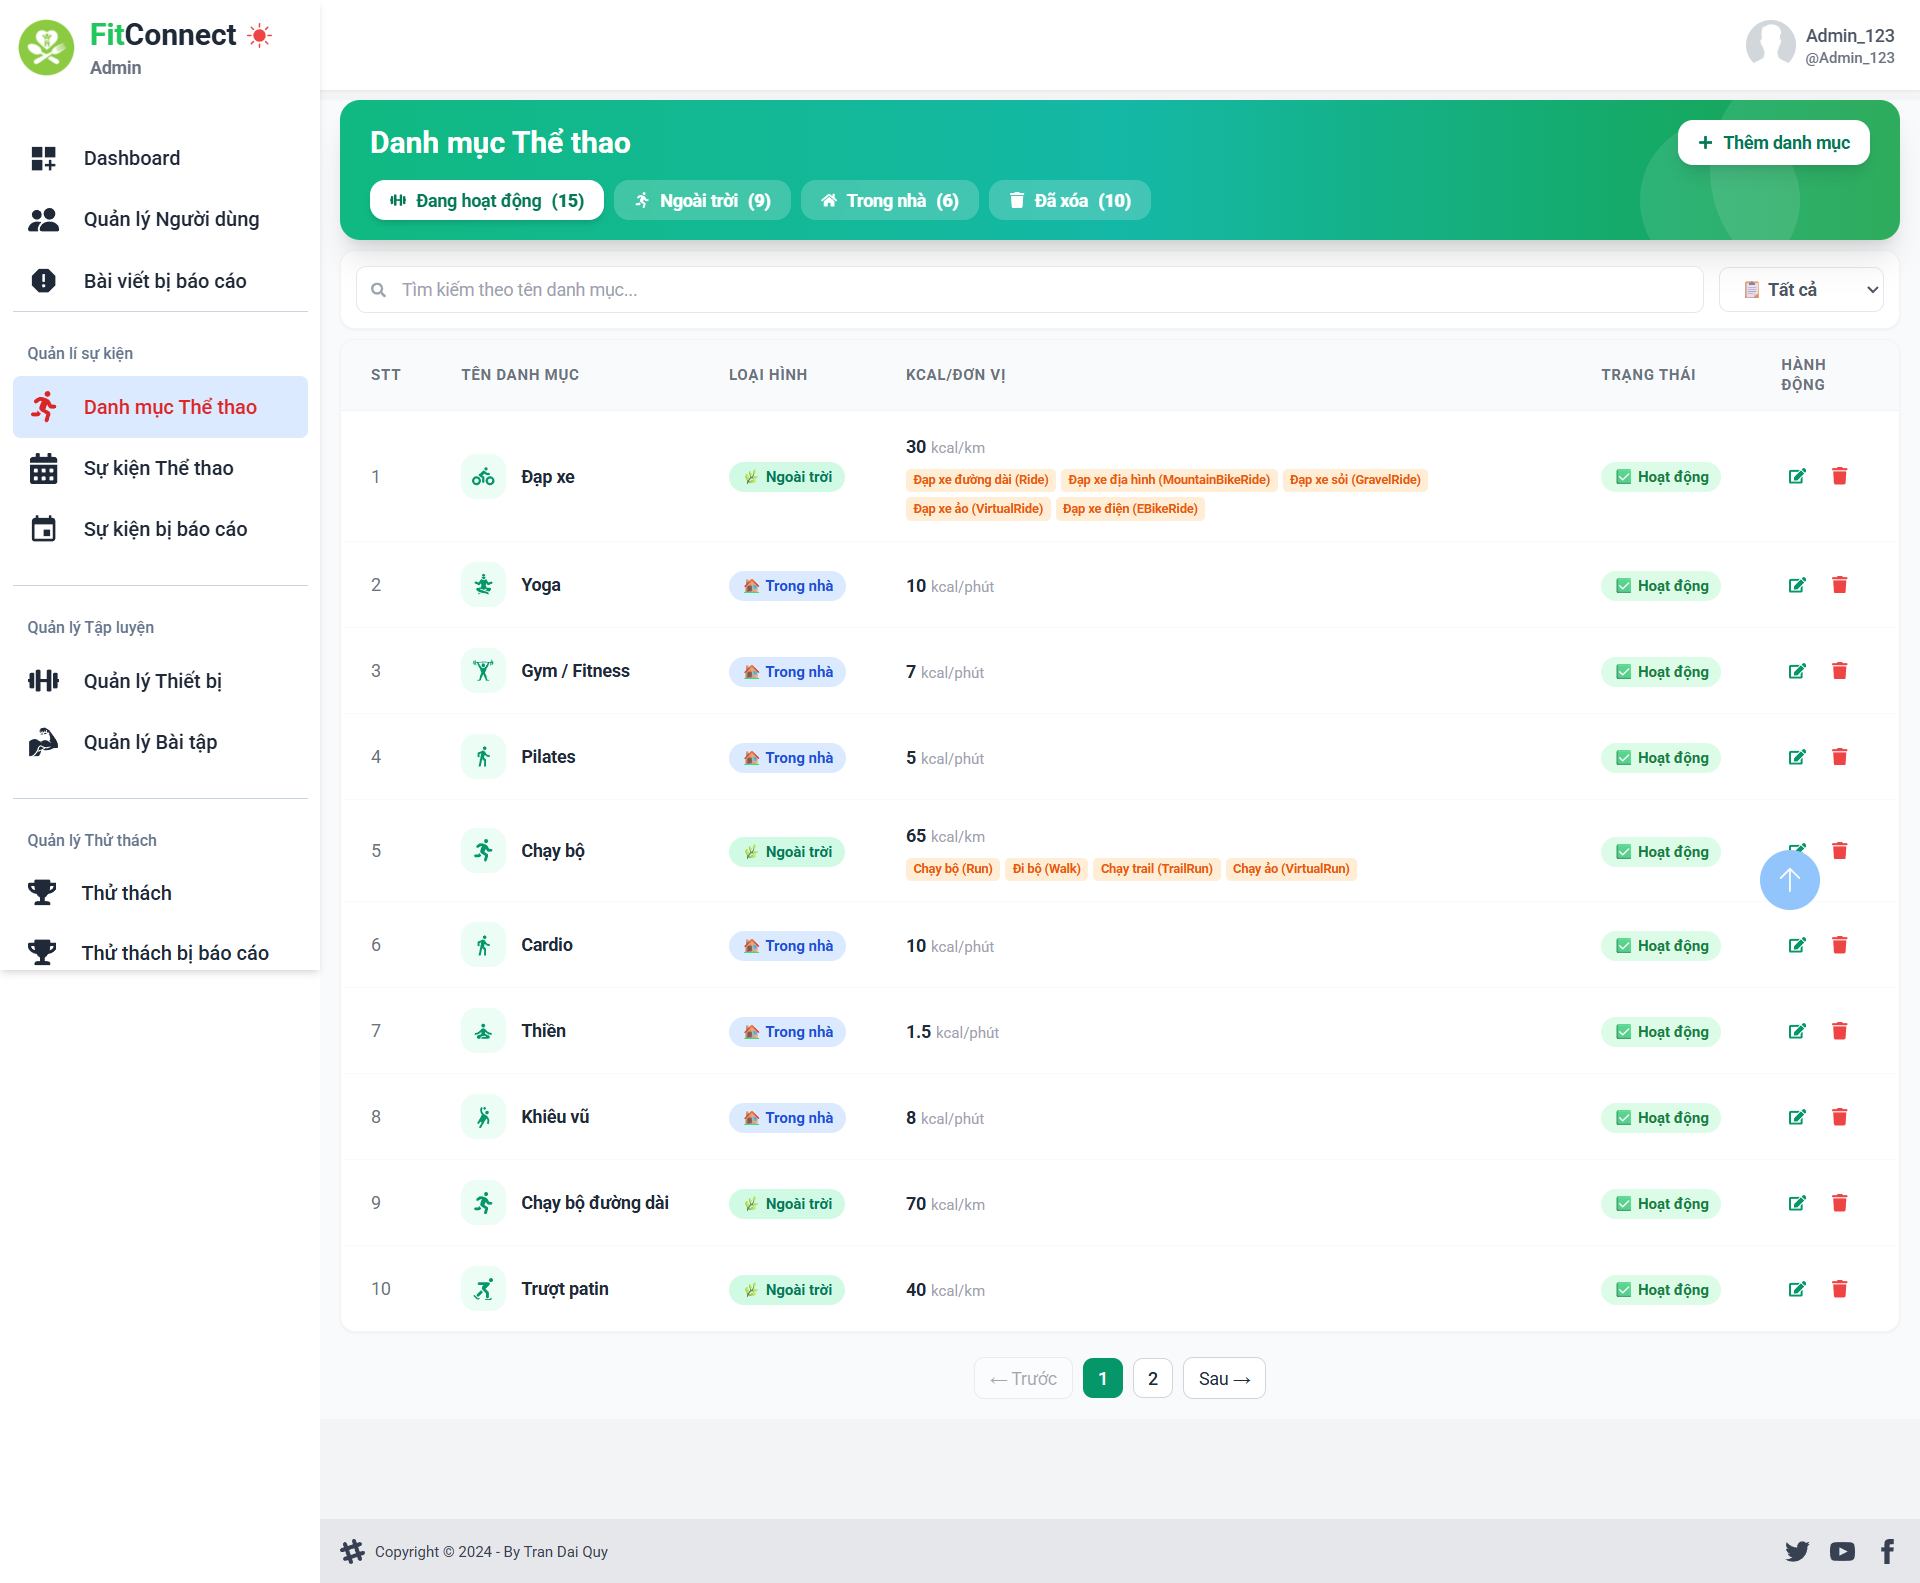
\includegraphics[width=0.85\textwidth]{Images/IMG/TrangAmin/quanlydanhmucthethao.jpg}
    \vspace{1em}
    \caption{(e) Quản lý danh mục thể thao}
    \label{fig:ui_danhmucthethao}
\end{figure}



\subsubsection{Đánh giá Prototype}
Bộ prototype đã được kiểm tra với nhóm người dùng thử nghiệm (beta testers) gồm 15 người từ các nhóm đối tượng khác nhau. Kết quả thu được cho thấy mức độ hài lòng trung bình đạt 4.2/5.0 điểm về tính dễ sử dụng và 4.5/5.0 điểm về tính thẩm mỹ. Các phản hồi tích cực tập trung vào việc giao diện trực quan, dễ điều hướng và hình ảnh hấp dẫn. Một số điểm cải thiện đã được ghi nhận và áp dụng vào phiên bản cuối cùng, bao gồm điều chỉnh kích thước font chữ, cải thiện contrast màu sắc cho accessibility, và tối ưu hóa các animation transitions.

\subsection{Bảng màu và Typography}
\label{subsec:ui_color_typography_retained}
\begin{itemize}
    \item \textbf{Bảng màu:} Cấu trúc hệ màu Tía và Xanh đậm làm chủ đạo (Indigo/Violet Hue) mang lại điểm tựa thị giác, điểm xuyết cùng hiệu ứng nền kính mờ (Glassmorphism), lấp đầy giao diện bằng một ngôn ngữ tươi mới chuẩn chỉnh phong thái năng động của môn khoa học công nghệ sức khỏe rèn luyện chuyên nghiệp. Đi kèm cùng màu nhấn (accent color) với ý đồ kêu gọi mạnh mẽ động tác tương tác ngay và luôn trên màn hình.
    \item \textbf{Typography:} Font chữ dễ đọc, hiện đại (Inter, Roboto, Montserrat). Phân cấp rõ ràng giữa tiêu đề, nội dung chính và phụ.
\end{itemize}


